\documentclass[12pt,a4paper,twoside,openright]{book}


               %%%%%%%%%%%%%%%%%%%%%%%%%%%%%%%%%%%%%%
               %    Scelta dei package da usare     %
               %%%%%%%%%%%%%%%%%%%%%%%%%%%%%%%%%%%%%%

\usepackage[english]{babel}
%\usepackage[latin1]{inputenc}
\usepackage[utf8]{inputenc}
\usepackage{amsmath,amsfonts,amssymb,amsthm}
\usepackage{deistesi}
\usepackage{fancyhdr}


               %%%%%%%%%%%%%%%%%%%%%%%%%%%%%%%%%%%%%%%%
               % Scelta delle dimensioni della pagina %
               %%%%%%%%%%%%%%%%%%%%%%%%%%%%%%%%%%%%%%%%

\setlength{\textwidth}{13.5cm}
\setlength{\textheight}{19cm}
\setlength{\footskip}{3cm}




               %%%%%%%%%%%%%%%%%%%%%%%%%%%%%%%%%%%%%%
               %  Informazioni generali sulla Tesi  %
               %    da usare nell'intestazione      %
               %%%%%%%%%%%%%%%%%%%%%%%%%%%%%%%%%%%%%%

\titolo{Applying the Reactive Programming Paradigm: Toward a More Declarative Application Development Approach}
\laureando{Alessandro Zoffoli}
\annoaccademico{2014--2015}
\scuola{}
\facolta{Ingegneria}
\corsodilaurea{CORSO DI LAUREA MAGISTRALE IN INGEGNERIA E SCIENZE INFORMATICHE}
\corso{Programmazione Avanzata e Paradigmi}
\relatore{Alessandro Ricci}
\corelatore{Philipp Haller}
\parolechiave{Reactive Programming}{Declarative}{Streams}{State}{Side effects}{}
\dedica{To my family.}
               %%%%%%%%%%%%%%%%%%%%%%%%%%%%%%%%%%%%%%
               % Fine Preambolo %
               % Inizio tesi     %
               %%%%%%%%%%%%%%%%%%%%%%%%%%%%%%%%%%%%%%

 \sessione{I}
               %%%%%%%%%%%%%%%%%%%%%%%%%%%%%%%%%%%%%%
               % Fine Preambolo %
               % Inizio tesi     %
               %%%%%%%%%%%%%%%%%%%%%%%%%%%%%%%%%%%%%%

\begin{document}

%%%%%%%%%%%%%%%%%%%%%%%%%
% inizio prefazione
%
% pagina del titolo, indice, sommario
%%%%%%%%%%%%%%%%%%%%%%%%%
\frontmatter \maketitle \pagestyle{plain} \tableofcontents
%``testo''

\chapter{Introduction}
\label{ch:intro}

After almost 10 years from ``The Free Lunch Is Over'' article, where the
need to parallelize programs started to be a real and mainstream issue,
a lot of stuffs did happened:

\begin{itemize}
\item
  Processor manufacturers are reaching the physical limits with most of
  their approaches to boosting CPU performance, and are instead turning
  to hyperthreading and multicore architectures;
\item
  Applications are increasingly need to support concurrency;
\item
  Programming languages and systems are increasingly forced to deal well
  with concurrency.
\end{itemize}

The article concluded by saying that we desperately need an higher-level
programming model for concurrency than languages offer today.

This thesis is an attempt to propose an overview of a paradigm that aims
to properly abstract the problem of propagating data changes:
\textbf{Reactive Programming} (RP). This paradigm propose an
\textbf{asynchronous non-blocking} approach to concurrency and
computations, abstracting from the low-level concurrency mechanisms.


The first chapter of this thesis will introduce the basics of RP, starting from simple abstractions and then exploring their main advantages and drawbacks.

The second chapter will present a detailed overview of some of the most popular and used frameworks that enable the developer to put RP principles in practice. This chapter will present the main abstractions and APIs for each framework, with a particular attention for the style and approach that the framework itself suggests in respect to the host language used.

The third chapter will propose an approach to solve a particular kind of modern applications: mobile applications. This chapter will consider iOS and Android as the reference platforms, and will then explore a common architectural approach to better express and implement mobile applications. It won't be a surprise that RP will have a central role in this chapter.

The fourth chapter will propose an approach to implement event processing application. This kind of applications will have an increasing role in our days, and RP expressiveness can be usefull to model and express applications that interact and compute a lot of real-time data.

Finally, the fifth chapter will conclude the thesis, with some final note and comparison.

%%%%%%%%%%%%%%%%%%%%%%%%%
% inizio corpo del documento
%
% sequenze dei vari capitoli
% � consigliato mantenere una struttura logica ben definita per separare i vari capitoli
% si consiglia di reificare tale struttura fisicamente sul file system
%%%%%%%%%%%%%%%%%%%%%%%%%

\mainmatter

% stile della pagina
\pagestyle{fancy} \fancyhead[LE,RO]{\bfseries\thepage}

% inclusione dei capitoli
\chapter{Reactive programming}\label{reactive-programming}

When using the imperative programming paradigm, the act of capturing
dynamic values is done only indirectly, through \textbf{state and
mutations}. In this context, the idea of \emph{dynamic/evolving} values
is not a first class value in the paradigm. Moreover, the paradigm can
only capture discrete evolving values, since the paradigm itself is
\emph{temporally discrete}.

Reactive programming is a programming paradigm that aims to provide a
more declarative way to abstract computations and mutations.

Wikipedia defines reactive programming as: 
\begin{quote} 
a programming paradigm oriented around data flows and the propagation of change. This
means that it should be possible to express static or dynamic data flows
with ease in the programming languages used, and that the underlying
execution model will automatically propagate changes through the data
flow.
\end{quote}

In this definition emerges some key concepts: 

\begin{itemize}
\itemsep1pt\parskip0pt\parsep0pt
\item
  expressing computations in terms of \textbf{data flows} 
\item
  \textbf{change is propagated} in a composable way 
\item
  the language or framework has to support \textbf{declarativeness} 
\item
  all the ``plumbing work'' is done by the execution model, ensuring that the actual 
  computation respects the semantics

\end{itemize}

One of the best examples to describe reactive programming is to think of
a spreadsheet, in which there're three cells, A, B and C and A is
defined as the sum of B and C. Whenever B or C changes, A updates
itself. The example is really simple and it's also something that we're
used to know. Reactive programming is all about propagating changes
throughout a system, automatically.

This chapter will focus on \textbf{Functional Reactive Programming} and
\textbf{Reactive Programming}, in an attempt to provide formal
definitions.

\section{Functional Reactive
Programming}\label{functional-reactive-programming}

Functional reactive programming has its origin with \emph{Fran}
(Functional reactive animation), a Haskell library for interactive
animations by Conal Elliott. Elliott found it difficult to express the
\emph{what} of an interactive animation abstracting from the \emph{how},
and built a set of expressive and recursive data types, combined with a
declarative programming language.

Informally, \textbf{functional reactive programming} is a programming
paradigm which brings a notion of \textbf{time} in the functional
programming paradigm, providing a conceptual framework for implementing
reactive systems. In fact, FRP let the application achieve reactivity by
providing constructs for specifying \emph{how behaviors change in
response to events}.

Elliott says that FRP is all about two main things: \emph{denotative}
and \emph{temporally continuos}. Infact, he also likes the term
``\emph{denotative, continuous-time programming}'' to replace functional
reactive programming, since it reduces the confusion.

Always about the \textbf{denotative} part, he means that the paradigm
should be founded on a precise, simple, implementation-independent,
compositional semantics that exactly specifies the meaning of each type
and building block. The compositional nature of the semantics then
determines the meaning of all type-correct combinations of the building
blocks.

From an Elliott's quote: 

\begin{quote}
Denotative is the heart and
essence of functional programming, and is what enables precise and
tractable reasoning and thus a foundation for correctness, derivation,
and optimization.
\end{quote}

About the \textbf{continuous time} part, there's some confusion. Some
claim that it's an idea somehow unnatural or impossible to implement
considering the discrete nature of computers. To this issues, Elliott
answers in the following way:

\begin{quote}
This line of thinking strikes me as bizarre, especially when coming from
Haskellers, for a few reasons: Using lazy functional languages, we
casually program with infinite data on finite machines. We get lovely
modularity as a result {[}\ldots{}{]}. There are many examples of
programming in continuous space, for instance, vector graphics,
{[}\ldots{}{]} I like my programs to reflect how I think about the
problem space rather than the machine that executes the programs, and I
tend to expect other high-level language programmers to share that
preference.
\end{quote}

Another name that Elliott suggests for continuous is
\emph{resolution-independent}, and thus able to be transformed in time
and space with ease and without propagating and amplifying sampling
artifacts. As an example, he propose the ``finite vs infinite'' data
structure issue:

\begin{quote}
We only access a finite amount of data \emph{in the end}. However,
allowing infinite data structures \emph{in the middle} makes for a much
more composable programming style. Each event has a stream (finite or
infinite) of occurrences. Each occurrence has an associated time and
value.
\end{quote}

Fran integrates general ideas from synchronous data-flow languages into
the non-strict, pure functional language Haskell. It takes a monadic
approach and encapsulates operations over time-varying values and
discrete events into data structures that are evaluated by an
interpreter loop. The main idea of FRP is to model user inputs as
functions that changes over time.


\subsection{Behaviors and Event Streams}\label{behaviors-and-event-streams}

FRP introduces two special abstractions:

\begin{itemize}
\itemsep1pt\parskip0pt\parsep0pt
\item
  \textbf{behaviors or signals}, values that are continuous functions of
  time.
\item
  \textbf{event streams}, values which are discrete functions of time.
\end{itemize}

\textbf{Behaviors} are dynamic/evolving values, and are first class
values in themselves. Behaviors can be defined and \emph{combined}, and
\emph{passed} into and out of functions.

Behaviors are built up out of a few primitives, like constant (static)
behaviors and time (like a clock), and then with sequential and parallel
combination. n-behaviors are combined by applying an n-ary function (on
static values), ``point-wise'', i.e., continuously over time.

In other terms, a Behavior simply \textbf{sends values over time} until
it either \textbf{completes}, or \textbf{errors out}, at which point it
stops sending values forever.

Examples of behaviours are the following:

\begin{itemize}
\itemsep1pt\parskip0pt\parsep0pt
\item
  time
\item
  a browser window frame
\item
  the cursor position
\item
  the position of an image during an animation
\item
  audio data
\item
  \ldots{}
\end{itemize}

\textbf{Events} enable to account for discrete phenomena, and each of it
has a stream (finite or infinite) of occurrences. Each occurrence is a
value paired with a time. Events are considered \emph{to be improving
list of occurrences}.

Formally, the points at which an event stream is defined are termed
\emph{events} and events are said to \emph{occur} on an \emph{event
stream}.

Example of event streams are the following:

\begin{itemize}
\itemsep1pt\parskip0pt\parsep0pt
\item
  timer events
\item
  key presses
\item
  mouse clicks
\item
  MIDI data
\item
  network packets
\item
  \ldots{}
\end{itemize}

Every instance of FRP conceptually includes both behaviors and events.
The classic instance of FRP takes behaviors and events as first-class
values.

\section{Evaluation model}\label{evaluation-model}

The core of languages that support Reactive Programming is about
\textbf{how changes are propagated}. From the programmer's point of view
this should be as much transparent as possible. In other words, a change
of a value is automatically propagated to all dependent computations
without the user has to manually propagate the changes by himself.

At the language level this means that there should be a mechanism that
is triggered when there's an event occurrence at an event source. This
mechanism will fire a notification about the changes to dependent
computations, that will possibly trigger a recomputation, and so on.

The issue of \emph{who initiates the propagation of changes} is a really
important decision in designing a language or a framework that supports
RP.

In simple terms the question is whether the source should \emph{push}
new data to its dependents (consumers) or the dependents should
\emph{pull} data from the event source (producer).

\begin{figure}[htbp]
\centering
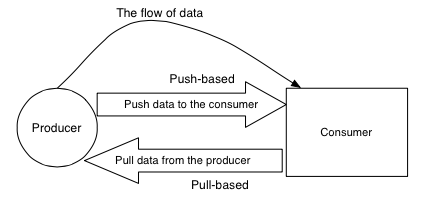
\includegraphics[scale=0.75]{imgs/eval.png}
\caption{Push- Versus Pull-based evaluation model, from the paper ``A
survey on Reactive Programming''}
\end{figure}

In the literature there are two main evaluation models:

\begin{itemize}
\itemsep1pt\parskip0pt\parsep0pt
\item
  \textbf{Pull-Based}, in which the computation that requires a value
  has to pull it from the source. The propagation is said to be
  \emph{demand-driven}. The pull model has been implemented in Fran,
  also thanks to the lazy evaluation of Haskell. A main trait of this
  approach is that the computation requiring the value has the liberty
  to only pull the new values when it actually needs it. From another
  point of view, this trait can lead to a significant latency between an
  occurrence of an event and when its reactions are triggered.
\item
  \textbf{Push-Based}, in which when the event source has new data it
  pushes the data to its dependent computations. The propagation is said
  to be \emph{data-driven}. An example of a recent implementation that
  use this model is Scala.React, that will be introduced later in this
  thesis. This approach also brings the issue of wasteful recomputation,
  since every new data that is pushed to the consumer triggers a
  recomputation.
\end{itemize}

Typically, reactive programming languages use \textbf{either a
pull-based or push-based model}, but there are also languages that
employ \textbf{both} approaches. In latter case there've both the
benefits of the push-based model (efficiency and low latency) and those
of the pull-based model (flexibility of pulling values based on demand).

\section{Glitches}\label{glitches}

A \textbf{glitch} is a \textbf{temporary inconsistency} in the
observable state. Due to the fact that updates do not happen
instantaneously, but instead take time to compute, the values within a
system may be \textbf{transiently out of sync} during the update
process. This may be a problem, depending on how tolerant the
application is of occasional stale inconsistent data. For example,
consider a computation that is run before all its dependent expressions
are evaluated and that can result in fresh values being combined with
stale values.

The paper ``A Survey on Reactive Programming'' by Bainomugisha et al.
depict the problem with the following program:

\begin{verbatim}
var1 = 1
var2 = var1 * 1
var3 = var1 + var2
\end{verbatim}

\begin{figure}[htbp]
\centering
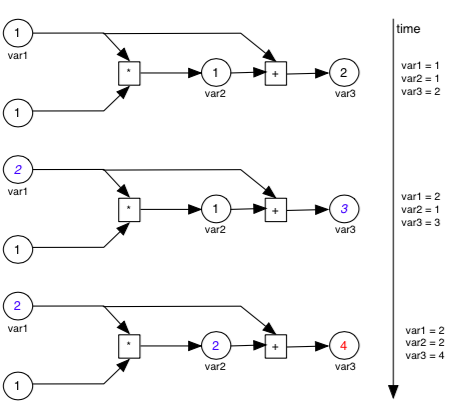
\includegraphics[scale=0.75]{imgs/glitches.png}
\caption{Momentary view of inconsistent program state and
recomputation.}
\end{figure}

The image related to the program above shows how the state of the
program results incorrect (\texttt{var3} is evaluated as 3 instead of 4)
and that this also leads to a wasteful recomputation (since
\texttt{var3} is computed one time more than the necessary).

Glitches only happens when using a \emph{push-based} evaluation model
and can be avoided by arranging expressions in a topologically sorted
graph. This implementation detail ensures that an expression is always
evaluated after all its dependants have been evaluated.

\section{Lifting}\label{lifting}

The term \emph{lifting} is used to depict the process of
\textbf{converting} an ordinary operator to a variant that can operate
on behaviors. This process is essential for the end user of the
language/framework, since it ensures conciseness and composability. In
other words, lifting is used to move from the non-reactive world to
reactive behaviors.

Lifting a \textbf{value} creates a \textbf{constant behavior} while
lifting a \textbf{function} \textbf{applies the function continuously}
to the argument behaviors. There is no similar lifting operation for
events, since an event would need an occurrence time as well as a value.

Lifting an operation can be formalized by the following definition,
assuming functions that only take one parameter (generalising to
functions that take multiple arguments is trivial):

\[
lift: f(T)  \rightarrow f_{lifted} (Behavior < T >).
\]

The \(f_{lifted}\) function can now be applied to behaviors that holds
values of type \(T\). Lifting enables the language or framework to
register a dependency graph in the application's dataflow graph.

Starting from the previous definition, the evaluation of a lifted
function called with a behavior at the time step \(i\) can be formalized
as follows:

\[
f_{lifted}(Behavior < T >)  \rightarrow f(T_i) .
\]

where \(T_i\) is the value of the behavior at the time step \(i\).


In the literature there are at least three main lifting strategies:

\begin{enumerate}
\def\labelenumi{\arabic{enumi}.}
\item
  \textbf{Implicit lifting}, that happens when an ordinary language
  operator is applied on a behaviour and it is automatically lifted.
  Implicit lifting is often used by dynamically typed languages.
  Formally: \[
  f(b1)  \rightarrow f_{lifted}(b1) .
  \]
\item
  \textbf{Explicit lifting}, usually used by statically typed languages.
  In this case the language provides a set of combinators to lift
  ordinary operators to operate on behaviors. Formally: \[
  lift(f)(b1)  \rightarrow f_{lifted}(b1) .
  \]
\item
  \textbf{Manual lifting}, when the language does not provide lifting
  operators. Formally: \[
  f(b1)  \rightarrow f(currentValue(b1)) .
  \]
\end{enumerate}


\section{Reactive confusion}\label{reactive-confusion}

In these days \textbf{reactive programming} and \textbf{functional
reactive programming} are two terms that create a lot of
\textbf{confusion}, and maybe are also over-hyped.

The definitions that come from Wikipedia are still pretty vague and only
Functional reactive programming introduced by Connal Elliott has a clear
and simple denotative semantics. In advance to this, Elliott himself
doesn't like the name he gave to the paradigm.

The concepts behind these newly introduced paradigms are pretty similar.
Reactive programming is a paradigms that facilitates the development of
applications by providing \textbf{abstractions} to express
\emph{time-varying values} and automatically propagating the
\emph{changes}: behaviors and events. Functional reactive programming
can be considered a ``sibling'' of reactive programming, providing
composable abstractions. Elliot identifies the key advantages of the
functional reactive programming paradigm as: \emph{clarity, ease of
construction, composability, and clean semantics}.

In 2013 Typesafe launched http://www.reactivemanifesto.org, which tried
to define what reactive applications are. The reactive manifesto didn't
introduce a new programming paradigm nor depicted RP as we intended RP
in this thesis. What the reactive manifesto did instead was to depict
some really relevant computer science principles about scalability,
resilience and event-driven architectures, and RP is one of the tools of
the trade.

Erik Meijer, in his talk ``Duality and the End of Reactive'', concluded
that all the hype and the buzzwords around the ``reactive world'' has no
sense, and that the core of the paradigm is \textbf{all about composing
side effects}. In his talk and related papers, he depicted the
\textbf{duality} that links enumerables and observables.

\begin{table}[]
\centering
\caption{The essential effects in programming}
\label{my-label}
\begin{tabular}{|l|l|l|}
\hline
             & {\bf One}     & {\bf Many}        \\ \hline
Synchronous  & T/Try{[}T{]}  & Iterable{[}T{]}   \\ \hline
Asynchronous & Future{[}T{]} & Observable{[}T{]} \\ \hline
\end{tabular}
\end{table}

In short, an enumerator is basically a getter with the ability to fail
and/or terminate. It might also return a future rather than a value. An
\textbf{iterable} is a getter that returns an \textbf{iterator}. If we
take the category-theoretic dual of these types we get the
\textbf{observer} and \textbf{observable} types. And this conclusion is
what let us to relate all the principal effects in programming, where in
one axis there's is the nature of the computation (sync or async) and in
the other one there's the cardinality of the result (one or many).

\chapter{State of the union}\label{state-of-the-union}

The previous chapter quickly introduces the basic notions of RP. This
chapter will give an overview of the state of the art for RP frameworks.

This thesis author arbitrarily choose four relevant libraries:

\begin{itemize}
\itemsep1pt\parskip0pt\parsep0pt
\item
  Scala.React
\item
  RxJava
\item
  ReactiveCocoa
\item
  Akka Streams
\end{itemize}

\section{Scala.React}\label{scala.react}

\textbf{Scala.React} is a framework that has been introduced with the
paper ``Deprecating the Observer Pattern'' from Maier, Odersky and
Rompf. The key concepts around Scala.React originate in Elliot's FRP,
and Scala.React aims to provide a \textbf{combinator-based approach for
reactive programming}.

The paper depicts how the observer pattern should be considered an
anti-pattern, since it violates a lot of software engineering principles
such as encapsulation, composability, separation of concerns,
scalability, uniformity, abstraction, semantic distance..

The authors aims to provide and depict an efficient use of
object-oriented, functional, and data-flow programming principles to
overcome the limitations of the existing approaches.

After many years from its presentation, the framework seems to be an
academic library that can be neglectable in favor of the RxScala/RxJava
library. For the author of this thesis, the paper is really meaningful
in the context of this thesis, since it introduces a set of abstractions
that are close to the original model of FRP from Elliot.

\subsection{Reactive}\label{reactive}

Following the idea to provide APIs that starts with basic event handling
and ends in an embedded higher-order dataflow language, the framework
introduces a generic trait \texttt{Reactive}, that factors out the
possible concrete abstractions in the following way:

\begin{verbatim}
trait Reactive[+Msg, +Now] {
    def current(dep: Dependant): Now
    def message(dep: Dependant): Option[Msg]
    def now: Now = current(Dependent.Nil)
    def msg: Msg = message(Dependent.Nil)
}
\end{verbatim}

The trait \texttt{Reactive} is defined based on two type parameters: one
for \textbf{the message type an instance emits} and one for \textbf{the
values it holds}.

Starting from the previous base abstraction, two further types can be
defined:

\begin{verbatim}
trait Signal[+A] extends Reactive[A,A]
trait Events[+A] extends Reactive[A,Unit]
\end{verbatim}

The difference between the two types can be seen directly in the types:

\begin{itemize}
\itemsep1pt\parskip0pt\parsep0pt
\item
  In \texttt{Signal}, \texttt{Msg} and \texttt{Now} types are identical.
\item
  In \texttt{Events}, \texttt{Msg} and \texttt{Now} types differ. In
  particular, the type for the type parameter \texttt{Now} is
  \texttt{Unit}. This means that for an instance of \texttt{Events} the
  notion of ``current value'' has no sense at all.
\end{itemize}

The two subclasses need to implement two methods, which obtain reactive's current message or value and create dependencies in a single
turn.

The next two sections will better examine the two abstraction introduced
here.

NB: the examples and code provided in this chapter have been taken
directly from the paper itself.

\subsubsection{Events}\label{events}

The first type to take in consideration is the \texttt{Event} type.

To simplify the event handling logic in an application, the framework
provides a general and uniform event interface, with
\texttt{EventSource}. An \texttt{EventSource} is an entity that can
\emph{raise} or \emph{emit} events at any time. For example:

\begin{verbatim}
val es = new EventSource[Int]
es raise 1
es raise 2
\end{verbatim}

To attach a side-effect in response to an event, an observer has to
\emph{observe} the event source, providing a closure. Continuing with
the previous example, the following code prints all events from the
event source to the console.

\begin{verbatim}
val ob = observe(es) { x =>
    println("Receiving " + x)
}
...
ob.dispose()
\end{verbatim}

\texttt{observe(\ )} returns an handle of the observer,that can be used
to uninstall and dispose the observer prematurely, via its
\texttt{dispose()} method. This is a common pattern in all of the other
frameworks/libraries presented in this thesis.

The basic types for events handling are pretty neat and simple to reason
about, since they are first-class values. The usage of these types
starts to be helpful only if combined with a set of operators, that
enables developers to build better and declarative abstraction.

For example, the \texttt{Events} trait defines some common operators as
follows:

\begin{verbatim}
def merge[B>:A](that: Events[B]): Events[B]
def map[B](f: A => B): Events[B]
def collect[B](p: PartialFunction[A, B]): Events[B]
\end{verbatim}

When building abstractions, the developer doesn't need to take care of
the events propagation, since the framework itself provides this.

\subsubsection{Signal}\label{signal}

The \textbf{Signal} type represents the other half of the story.

In programming a large set of problems is about \textbf{synchronizing
data that changes over time}, and signals are introduced to overcome
these needs.

In simple words, a \texttt{Signal} is the \textbf{continuous}
counterpart of trait \texttt{Events} and represents \textbf{time-varying
values}, maintaining:

\begin{itemize}
\itemsep1pt\parskip0pt\parsep0pt
\item
  its \textbf{current value}
\item
  the current \textbf{expression} that defines the signal value
\item
  a set of \textbf{observers}: the other signals that depend on its
  value
\end{itemize}

A concrete type for \texttt{Signal} is the \texttt{Var}, that abstract
the notion of \textbf{variable signal} and is defined as follows:

\begin{verbatim}
class Var[A](init: A) extends Signal[A] {
    def update(newValue: A): Unit = ...
}
\end{verbatim}

A \texttt{Var}'s current value can change when somebody calls an
\texttt{update(\ )} operation on a it or the value of a dependant signal
changes.

\textbf{Constant signals} are represented by \texttt{Val}:

\begin{verbatim}
class Val[A](value: A) extends Signal[A]
\end{verbatim}

To compose signals, the framework doesn't provide combinator methods at
all, but introduce the notion of \textbf{signal expressions}, indeed. To
better explain the concept, let's look at a simple example.

\begin{verbatim}
val a = new Var(1)
val b = new Var(2)
val sum = Signal{ a()+b() }

observe(sum) { x => println(x) }

a()= 7
b()= 35
\end{verbatim}

Signals are primarily used to create variable dependencies as seen
above. In other words, the framework itself already performs all the “plumbing work” of connecting the dependencies and propagating the changes.

The framework and the Scala language provide a convenient and simple
syntax to get and update the current value of a Signal, and also to
create variable dependencies between signals. For example:

\begin{itemize}
\itemsep1pt\parskip0pt\parsep0pt
\item
  the code \texttt{Signal\{\ a()+b()\ \}} creates a dependencies that
  binds the changes from \texttt{a} and \texttt{b} to be propagated and
  evaluated in the \texttt{sum} signal
\item
  the code \texttt{a()=\ 7} is evaluated as \texttt{a.update(7)}
\item
  the framework also provide an implicit converter that enables to
  create easily \texttt{Val} signals
\end{itemize}


\subsection{Evaluation model}\label{evaluation-model}

Scala.React's propagation model is \textbf{push-driven}, and uses a
\textbf{topologically ordered dependency graph}. This implementation
detail ensures that an expression is always evaluated after all its
dependants have been evaluated, so glitches can't happen.

Scala.React proceeds in \textbf{propagation cycles}. The system is
\emph{either in a propagation cycle or}, if there are no pending changes
to any reactive, \emph{idle}. The model of \textbf{time} the system use
is a \textbf{discrete} one.

Every propagation cycle has two phases: first, all reactives are
synchronized so that observers, which are run in the second phase,
cannot observe inconsistent data. During a propagation cycle, the
reactive world is paused, i.e., no new changes are applied and no source
reactive emits new events or changes values.

A propagation cycle proceeds as follows:

\begin{enumerate}
\def\labelenumi{\arabic{enumi}.}
\itemsep1pt\parskip0pt\parsep0pt
\item
  Enter all modified/emitting reactives into a priority queue with the
  priorities being the reactives' levels.
\item
  While the queue is not empty, take the reactive on the lowest level
  and validate its value and message. The reactive decides whether it
  propagates a message to its dependents. If it does so, its dependents
  are added to the priority queue as well.
\end{enumerate}

\section{RxJava}\label{rxjava}

The table represents a possible classification of the
\textbf{effects} in programming.

\begin{table}[]
\centering
\caption{The essential effects in programming}
\label{my-label}
\begin{tabular}{|l|l|l|}
\hline
             & {\bf One}     & {\bf Many}        \\ \hline
Synchronous  & T/Try{[}T{]}  & Iterable{[}T{]}   \\ \hline
Asynchronous & Future{[}T{]} & \textbf{Observable{[}T{]}} \\ \hline
\end{tabular}
\end{table}

All the theory and the development of the reactive extensions libraries
started with an intuition of Erik Meijer, that theorized that
\textbf{iterable/iterator} are \textbf{dual} to
\textbf{observable/observer}. And this hypothesis is what let us to
relate all the principal effects in programming, where in one axis
there's is the nature of the computation (sync or async) and in the
other one there's the cardinality of the result (one or many).

The appendix on \textbf{futures and promises} covers the case of a
computation that returns a \textbf{single value}. This chapter will
focus on the abstraction of \textbf{Observables}, analyzing RxJava as a
case of study.

As the title of the repository states, \emph{RxJava is a library for
composing asynchronous and event-based programs using observable
sequences for the JVM}.

The library was heavily inspired by Rx.NET by Microsoft and is
developed by Netflix and other contributors. The code is open source
and recently, after 2 years of development, has reached the 1.0 version.

RxJava is also conform to the Reactive Streams initiative (see the
appendix), and this means that the hard problem of propagating and
reacting to back-pressure has been incorporated in the design of RxJava
already, and also that it interoperate seamlessly with all other
Reactive Streams implementations.

\subsection{Observable}\label{observable}

The fundamental entity of RxJava is the \textbf{Observable} type. An
observable is a \emph{sequence of ongoing event ordered in time}.

An \texttt{Observable} can emit 3 types of item:

\begin{itemize}
\itemsep1pt\parskip0pt\parsep0pt
\item
  values
\item
  error
\item
  completion event
\end{itemize}

RxJava provides a really nice documentation, with also some graphical
diagrams, called marble diagrams.

\begin{figure}[htbp]
\centering
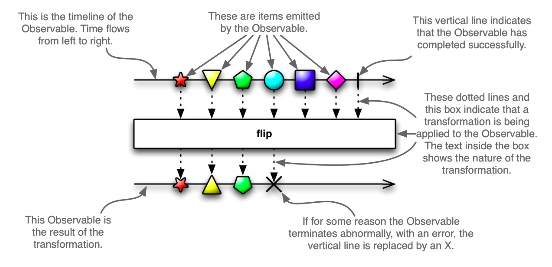
\includegraphics[scale=0.75]{imgs/marble.png}
\caption{A marble diagram}
\end{figure}

A marble diagram depicts how a an \texttt{Observable} and an
\texttt{Operator} behave:

\begin{itemize}
\itemsep1pt\parskip0pt\parsep0pt
\item
  observables are timelines with sequence of symbols
\item
  operators are rectangles, that accepts in input the upper observable
  and return in output the lower one
\end{itemize}

In RxJava, an \texttt{Observable} is defined over a generic type
\texttt{T}, the type of its values, as follows:

\begin{verbatim}
class Observable<T> { ... }
\end{verbatim}

An \texttt{Observable} can emit - in order - \textbf{zero, one or more
values, an error or a completion event}.

An \texttt{Observable} is an \textbf{immutable} entity, so the only way
to change the sequence of values it emits is through the application of
an \textbf{operator} and the subsequent creation of a new
\texttt{Observable}.

An entity can subscribe its interest in the values coming from an
\texttt{Observalbe} through its \texttt{subscribe(\ )} method, that
accepts one, two or three \texttt{Action} parameters (that correspond to
the \texttt{onNext(\ )}, \texttt{onError(\ )} and
\texttt{onComplete(\ )} callbacks).

The classic ``Hello, World'' example in RxJava and Java 8 is the
following:

\begin{verbatim}
Observable.just("Hello, world!").subscribe(s -> System.out.println(s));
\end{verbatim}

The \texttt{Observable} type provides some convenience methods that
return an observable with the given specification. An incomplete list
of these is the following:

\begin{itemize}
\itemsep1pt\parskip0pt\parsep0pt
\item
  \texttt{just(\ )}: convert an object or several objects into an
  Observable that emits that object or those objects
\item
  \texttt{from(\ )}: convert an Iterable, a Future, or an Array into an
  Observable
\item
  \texttt{empty(\ )}: create an Observable that emits nothing and then
  completes
\item
  \texttt{error(\ )}: create an Observable that emits nothing and then
  signals an error
\item
  \texttt{never(\ )}: create an Observable that emits nothing at all
\item
  \texttt{create(\ )}: create an Observable from scratch by means of a
  function
\item
  \texttt{defer(\ )}: do not create the Observable until a Subscriber
  subscribes; create a fresh Observable on each subscription
\item
  \ldots{}
\end{itemize}

Usually, observables created with these methods are used in conjunction
with other observables and operators, to create more complex logics.

\subsubsection{Operator}\label{operator}

In RxJava, operators are what enable the developer to \textbf{model} the
actual computation. An operator allows performing \textbf{almost every
type of manipulation} on the source observer in a declarative way.

Expressing a computation in terms of a stream of values is translated in
building a \textbf{chain of proper operators}. Usually, looking at the
signatures and at the types of the operators is really helpful when
choosing which operator is the right one for the goal to achieve.

An operator, to be applicable to an Observable, has to implement the
\texttt{Operator} interface and has to be lifted. The \texttt{lift}
function lifts a function (inside an \texttt{Operator}) to the current
Observable and returns a new Observable that when subscribed to will
pass the values of the current Observable through the \texttt{Operator}
function.

Operators are methods of the \texttt{Observable} class, so creating a
chain of operators starting from a source observable is a pretty
straightforward process.

RxJava provides a huge set of operators, and a lot of them is defined
in terms of other ones. What follows is only a small introductive
subset.

\subsubsubsection{Map}\label{map}

\texttt{Map} is an operator that returns an Observable that
\textbf{applies a specified function to each item} emitted by the source
Observable and emits the results of these function applications. Its
marble diagram is the following.

\begin{figure}[htbp]
\centering
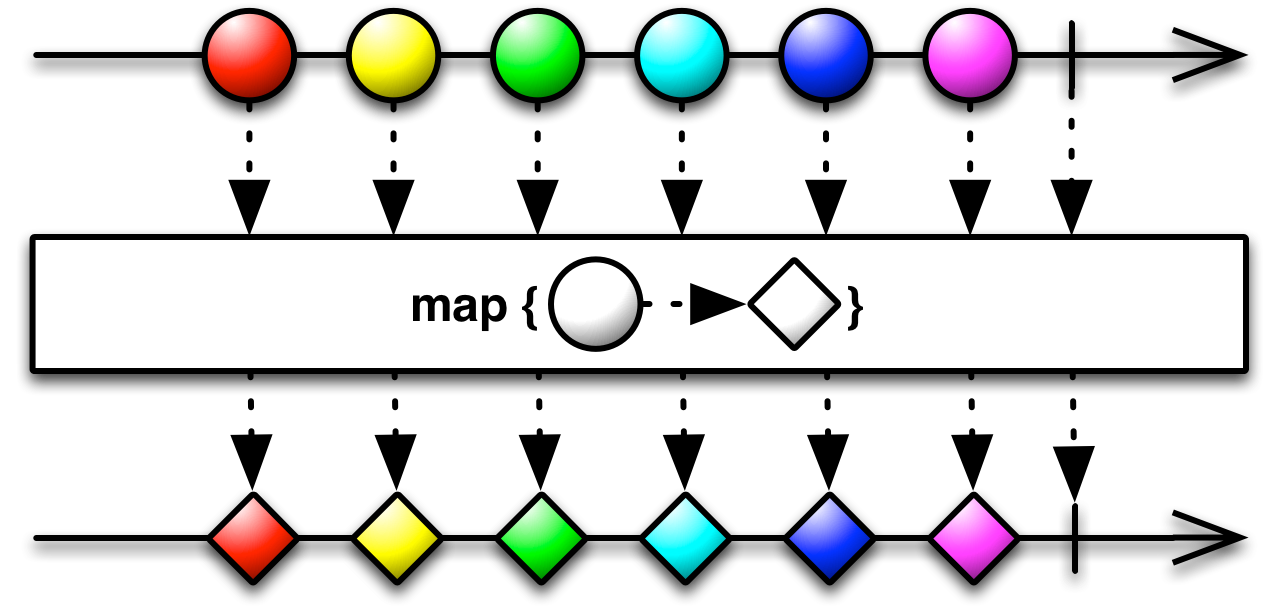
\includegraphics[scale=0.5]{imgs/map.png}
\caption{Map operator}
\end{figure}

To better clarify the concept of lifting introduced previously, let's
also look at the definition and implementation for \texttt{Map}.

\begin{verbatim}
public final <R> Observable<R> map(Func1<? super T, ? extends R> func) {
  return lift(new OperatorMap<T, R>(func));
}

...

public final class OperatorMap<T, R> implements Operator<R, T> {

    private final Func1<? super T, ? extends R> transformer;
    public OperatorMap(Func1<? super T, ? extends R> transformer) {
        this.transformer = transformer;
    }

    public Subscriber<? super T> call(final Subscriber<? super R> o) {
        return new Subscriber<T>(o) {

            public void onCompleted() {
                o.onCompleted();
            }

            public void onError(Throwable e) {
                o.onError(e);
            }

            public void onNext(T t) {
                try {
                    o.onNext(transformer.call(t));
                } catch (Throwable e) {
                    onError(OnErrorThrowable.addValueAsLastCause(e, t));
                }
            }
        };
    }
}
\end{verbatim}

\subsubsubsection{FlatMap}\label{flatmap}

\texttt{FlatMap} returns an Observable that \textbf{emits items based on
applying a function that is supplied to each item emitted by the source
Observable, where that function returns an Observable}, and then merging
those resulting Observables and emitting the results of this merger.

\begin{figure}[htbp]
\centering
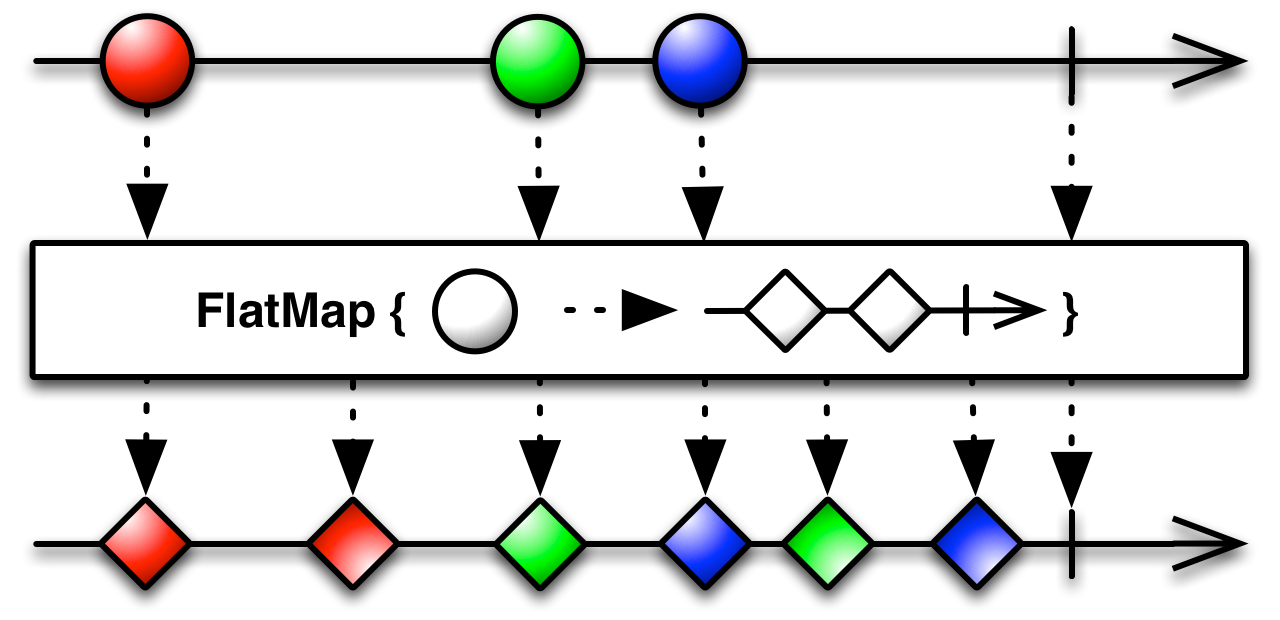
\includegraphics[scale=0.5]{imgs/flatMap.png}
\caption{FlatMap operator}
\end{figure}

\subsubsubsection{Filter}\label{filter}

\texttt{Filter} is quite obvious.

\begin{figure}[htbp]
\centering
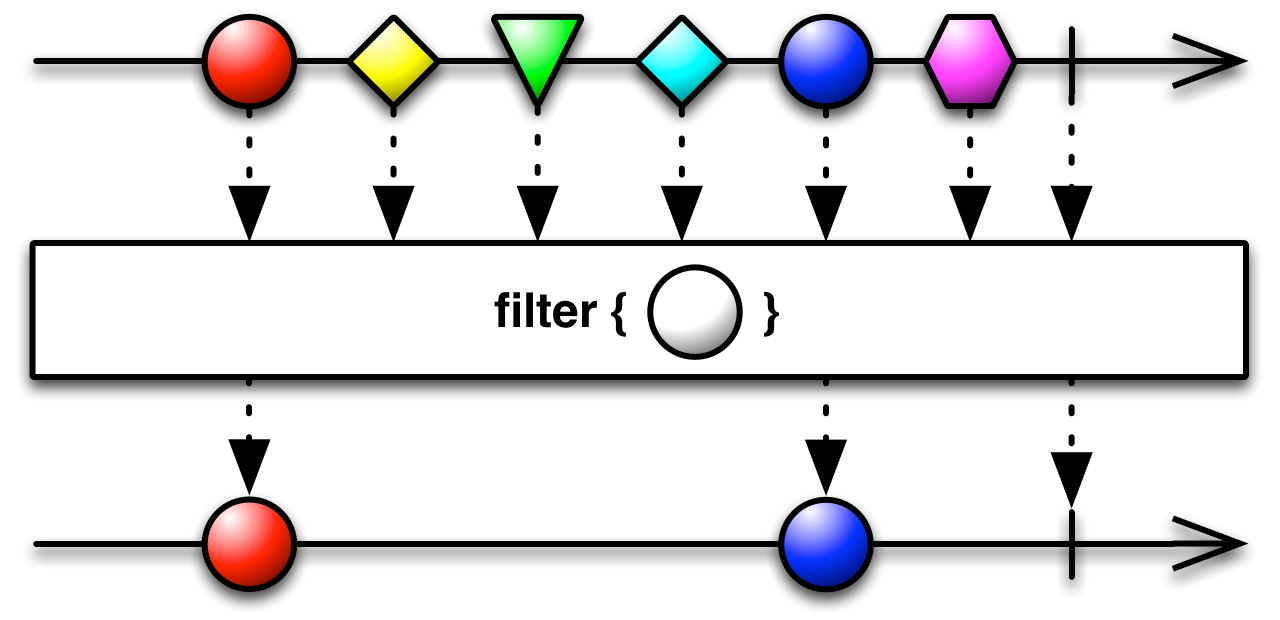
\includegraphics[scale=0.5]{imgs/filter.png}
\caption{Filter operator}
\end{figure}

\subsubsubsection{Scan}\label{scan}

\texttt{Scan} returns an Observable that \textbf{applies a specified
accumulator function} to the first item emitted by a source Observable,
then \textbf{feeds the result of that function along} with the second
item emitted by the source Observable into the same function, and so on
until all items have been emitted by the source Observable, and emits
the final result from the final call to your function as its sole item.

\begin{figure}[htbp]
\centering
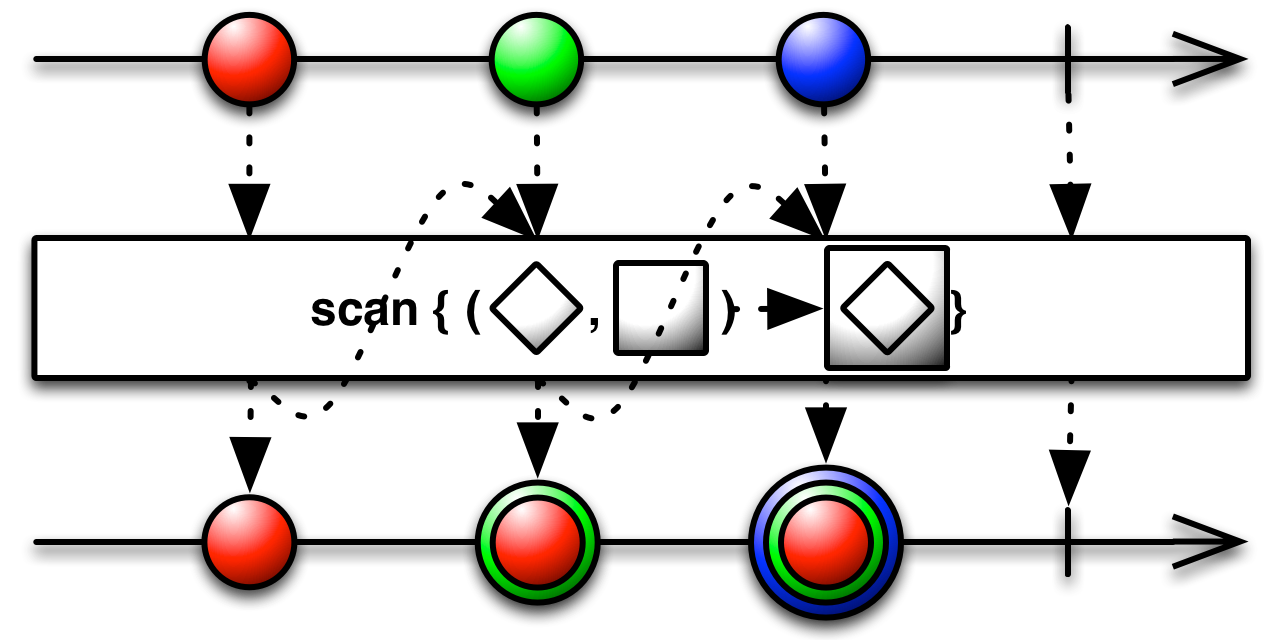
\includegraphics[scale=0.5]{imgs/scan.png}
\caption{Scan operator}
\end{figure}

\subsubsubsection{Take}\label{take}

\texttt{Take} returns an Observable that emits only the first n items
emitted by the source Observable.

\begin{figure}[htbp]
\centering
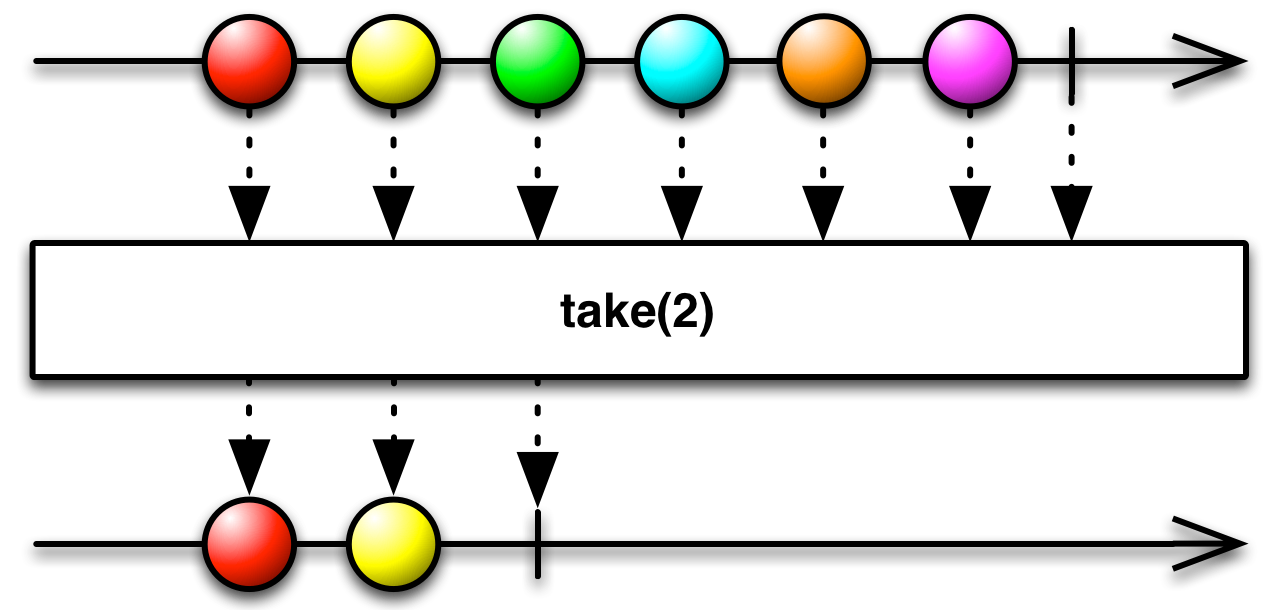
\includegraphics[scale=0.5]{imgs/take.png}
\caption{Take operator}
\end{figure}

\subsubsubsection{A complex example}\label{a-complex-example}

\begin{verbatim}
// Returns a List of website URLs based on a text search
Observable<List<String>> query(String text) { ... }

// Returns the title of a website, or null if 404
Observable<String> getTitle(String URL){ ... }

query("Hello, world!")                    // -> Observable<List<String>>
  .flatMap(urls -> Observable.from(urls)) // -> Observable<String>
  .flatMap(url -> getTitle(url))          // -> Observable<String>
  .filter(title -> title != null)
  .doOnNext(title -> saveTitle(title))    // extra behavior
  
  // -> Observable<Pair<Integer, String>>
  .map(title -> new Pair<Integer, String>(0, title)) 
  .scan((sum, item) -> new Pair<Integer, Word>(sum.first + 1, item.second))
  .take(5)
  .subscribe(indexItemPair ->
      System.out.println("Pos: " + indexItemPair.first + ": title:" + 
      							   indexItemPair.second ));
\end{verbatim}

The example starts with the hypothesis of having two methods that
returns observable, for example coming from the network layer of an
application. \texttt{query} return a list of url given a text and
\texttt{getTitle} returns the title of a website or null.

The computation aims to return all the title of the websites that match
the ``Hello, World!'' string.

The code itself is pretty self-explanatory, and shows how concise and
elegant a computation can be using the approach suggested by RxJava in
respect to its imperative-style counterpart.

\subsubsection{Error handling}\label{error-handling}

The previous sections introduced the basics of \texttt{Observable} and
\texttt{Operator}. This section will introduce how errors are handled in
RxJava.

As introduced previously, every Observable ends with either a single
call to \texttt{onCompleted()} \textbf{or} \texttt{onError()}.

What follows is an example of a chain of operators that contains some
transformation that may also fail.

\begin{verbatim}
Observable.just("Hello, world!")
  .map(s -> potentialException(s))
  .map(s -> anotherPotentialException(s))
  .subscribe(new Subscriber<String>() {
      @Override
      public void onNext(String s) { System.out.println(s); }

      @Override
      public void onCompleted() { System.out.println("Completed!"); }

      @Override
      public void onError(Throwable e) { System.out.println("Ouch!"); }
    });
\end{verbatim}

The \texttt{onError()} callback is called if an \texttt{Exception} is
thrown \textbf{at any time} in the chain, thus the operators don't have
to handle exceptions in first place since they are \textbf{propagated}
to the \texttt{Subscriber}, which has to manage all the error handling.


\subsection{Subscription}\label{subscription}

In RxJava, \texttt{Subscription} is an abstraction that represents the
\textbf{link} between an \texttt{Observable} and a \texttt{Subscriber}.

A subscription is a quite simple type:

\begin{verbatim}
public interface Subscription {
    public void unsubscribe();
    public boolean isUnsubscribed();
}
\end{verbatim}

The main usage for subscription is in its \texttt{unsubscribe(\ )}
method, that can be used to \emph{stop} the chain, \textbf{terminating
wherever it is currently executing code}.

\texttt{CompositeSubscription} is another useful type, that simplify the
management of multiple and related subscriptions. A composite
subscription comes with an algebra that defines the behaviors of its
methods:

\begin{itemize}
\itemsep1pt\parskip0pt\parsep0pt
\item
  \texttt{add(Subscription\ s)}, \textbf{adds a new Subscription} to the
  CompositeSubscription; if this is unsubscribed, will explicitly
  unsubscribing the new Subscription as well
\item
  \texttt{remove(Subscription\ s)}, \textbf{removes a Subscription} from
  the CompositeSubscription, and unsubscribes the Subscription
\item
  \texttt{unsubscribe()}, unsubscribes to \textbf{all} subscriptions in
  the CompositeSubscription
\item
  unsubscribing inner subscriptions has no effect on the composite
  subscription
\end{itemize}


\subsection{Scheduler}\label{scheduler}

In the previous sections a lot of concepts have been introduced. This
section will cover one of the most important aspects of the framework:
\textbf{schedulers}.

A scheduler is an \emph{object that schedules unit of work}, and it's
implemented through the the \texttt{Scheduler} type. This type allows to
specify \textbf{in which execution context} the chain or part of the
chain has to run. In particular, the developer can choose in which
thread:

\begin{itemize}
\itemsep1pt\parskip0pt\parsep0pt
\item
  an \texttt{Observable} has to run, with \texttt{subscribeOn(\ )}
\item
  a \texttt{Subscriber} has to run, with \texttt{observeOn(\ )}
\end{itemize}

The framework already provide some schedulers: 

\begin{itemize}
\itemsep1pt\parskip0pt\parsep0pt
\item
  \texttt{immediate(\ )},
that executes work \textbf{immediately} on the current thread
\item
  \texttt{newThread(\ )}, that creates a \textbf{new Thread} for each job
\item
  \texttt{computation(\ )}, that can be used for \textbf{event-loops},
processing callbacks and other computational work 
\item
  \texttt{io(\ )},
that is intended for \textbf{IO-bound} work, based on an Executor
thread-pool that will grow as needed
\end{itemize}

A really nice feature is the fact that applying the execution of a chain
to a particular scheduler doesn't break the chain of operators, keeping
the code clean and with a good level of declarativness.

An example of usage of schedulers is the following, in which an image is
fetched from the network and then processed. A network request is a
typical io-bound operation and it's performed in \texttt{io()}
scheduler, while a processing operation is a cpu-bound operation and
it's performed in a \texttt{computation()} scheduler.

\begin{verbatim}
myObservableServices.retrieveImage(url)
  .subscribeOn(Schedulers.io())
  .observeOn(Schedulers.computation())
  .subscribe(bitmap -> processImage(bitmap));
\end{verbatim}


\subsection{Subject}\label{subject}

\textbf{Subject} is a further entity that is provided by the framework.
A \texttt{Subject} is a sort of bridge or proxy that acts both as an
observer and as an \texttt{Observable}:

\begin{itemize}
\itemsep1pt\parskip0pt\parsep0pt
\item
  because \textbf{it is an observer}, it can \textbf{subscribe} to one
  or more observables
\item
  because \textbf{it is an Observable}, it can pass through the items it
  observes by \textbf{re-emitting} them, and it can also \textbf{emit}
  new \textbf{items}
\end{itemize}

\texttt{Subject} has the ``power'' of \textbf{turning a cold observable
hot}. In fact, when a \texttt{Subject} subscribes to an
\texttt{Observable}, it will trigger that \texttt{Observable} to begin
emitting items (and if that \texttt{Observable} is ``cold'' --- that is,
if it waits for a subscription before it begins to emit items). This can
have the effect of making the resulting \texttt{Subject} a ``hot''
\texttt{Observable} variant of the original ``cold''
\texttt{Observable}.

The framework provides a wide range of subjects, each one with its own
semantics. What follows is an overview of the main popular and used.

\subsubsection{PublishSubject}\label{publishsubject}

\begin{figure}[htbp]
\centering
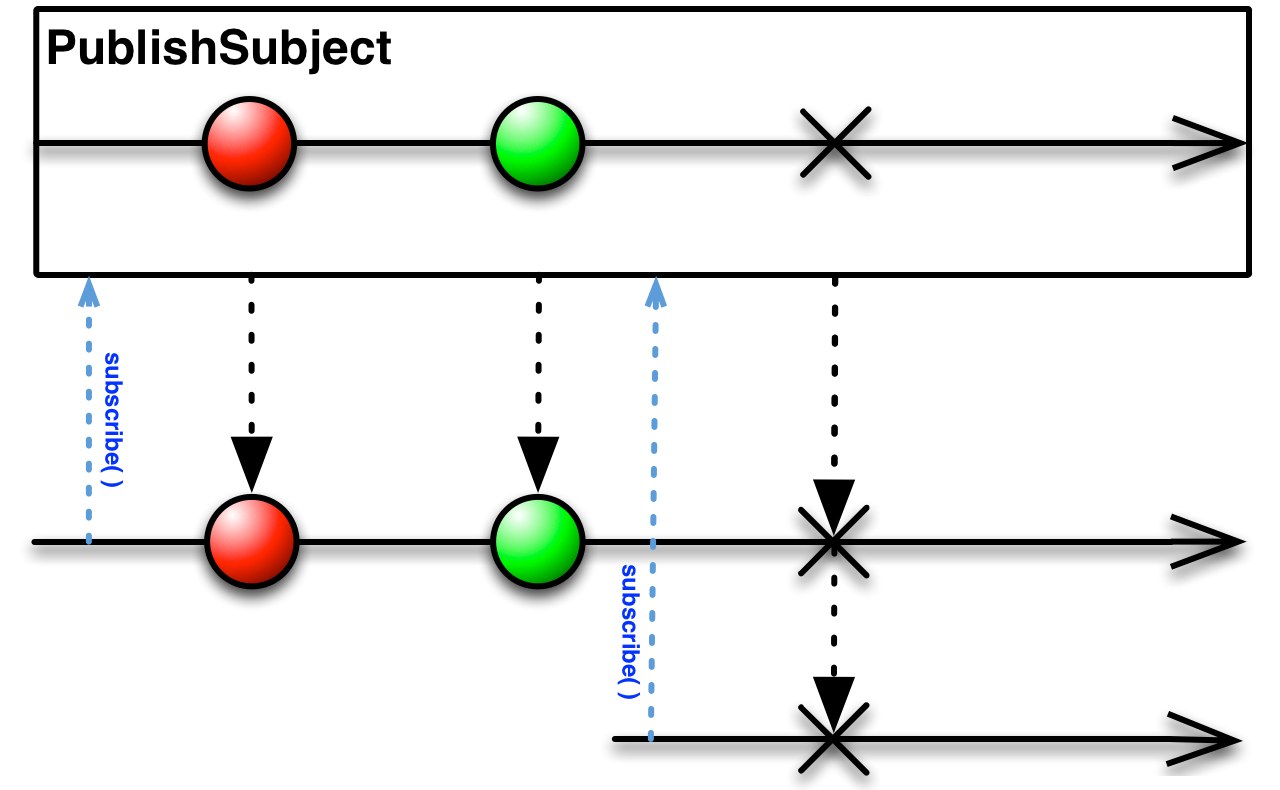
\includegraphics[scale=0.5]{imgs/pubsubj.png}
\caption{PublishSubject}
\end{figure}

\texttt{PublishSubject} emits to an observer only those items that are
emitted by the source Observable(s) \textbf{subsequent} to the time of
the subscription. This means that an observer will not receive the
previous emitted items.

\subsubsection{ReplaySubject}\label{replaysubject}

\begin{figure}[htbp]
\centering
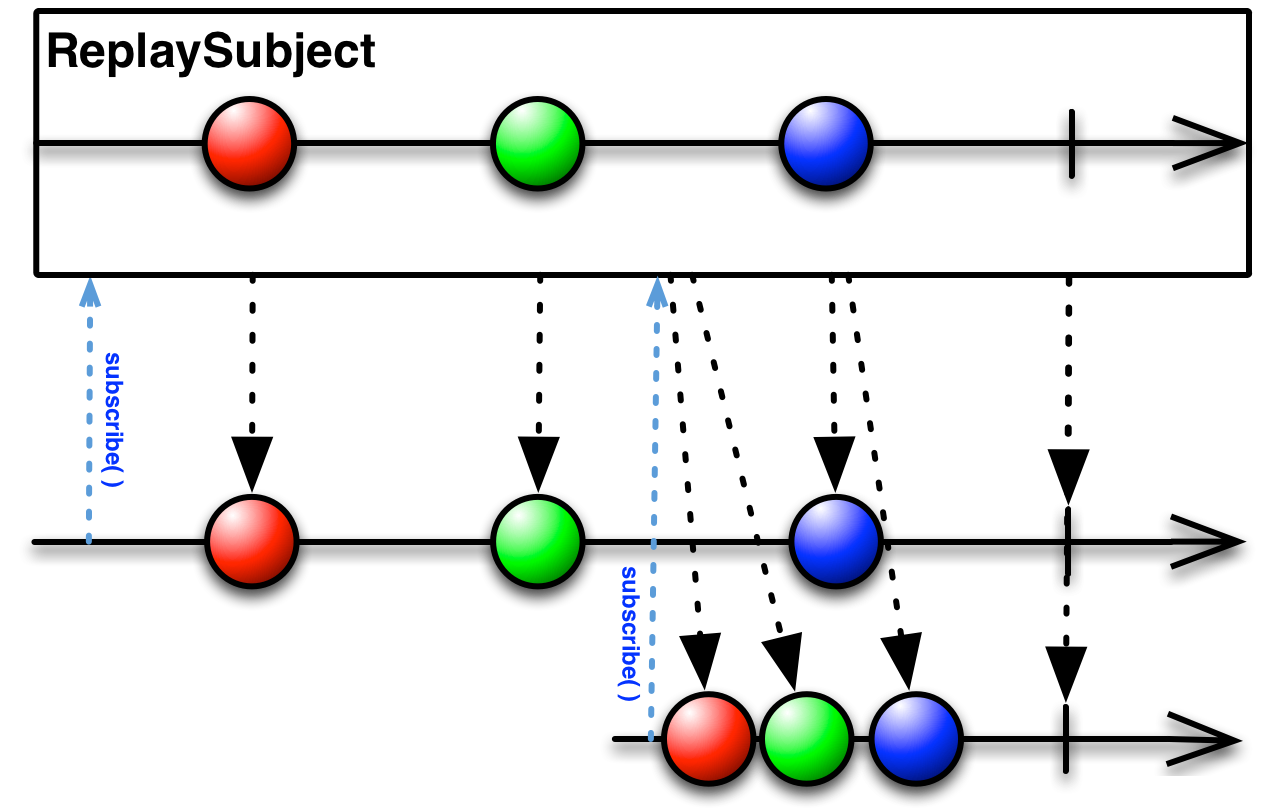
\includegraphics[scale=0.5]{imgs/replaysub.png}
\caption{ReplaySubject}
\end{figure}

\texttt{ReplaySubject} emits to any observer \textbf{all} of the items
that were emitted by the source Observable(s), regardless of when the
observer subscribes. To keep the memory consumption limited, this subject
also use a bounded buffer that enable to discard old items when the
limit size has been reached.

\subsubsection{AsyncSubject}\label{asyncsubject}

\begin{figure}[htbp]
\centering
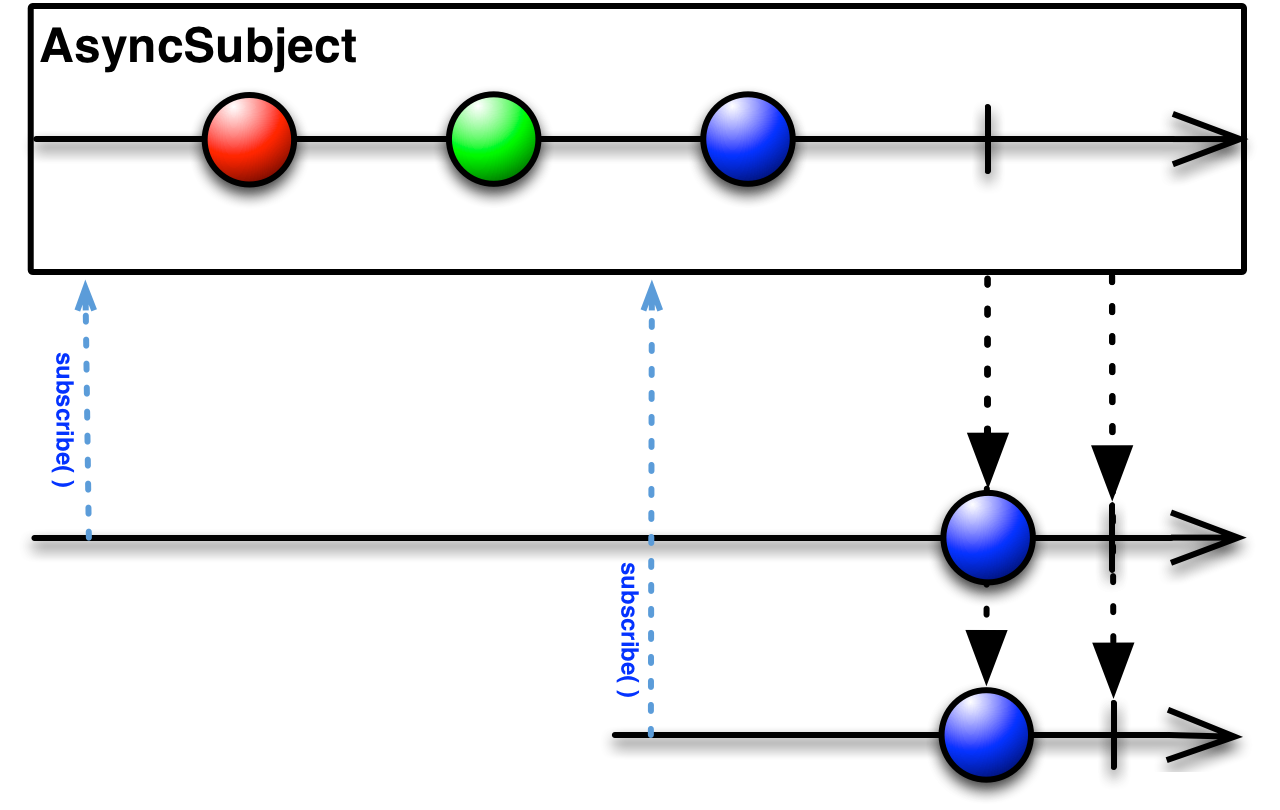
\includegraphics[scale=0.5]{imgs/asyncsubj.png}
\caption{AsyncSubject}
\end{figure}

An \texttt{AsyncSubject} caches and only remember the \textbf{last}
value of the Observable, and only after that source Observable completes
emits that value.

\subsubsection{BehaviorSubject}\label{behaviorsubject}

\begin{figure}[htbp]
\centering
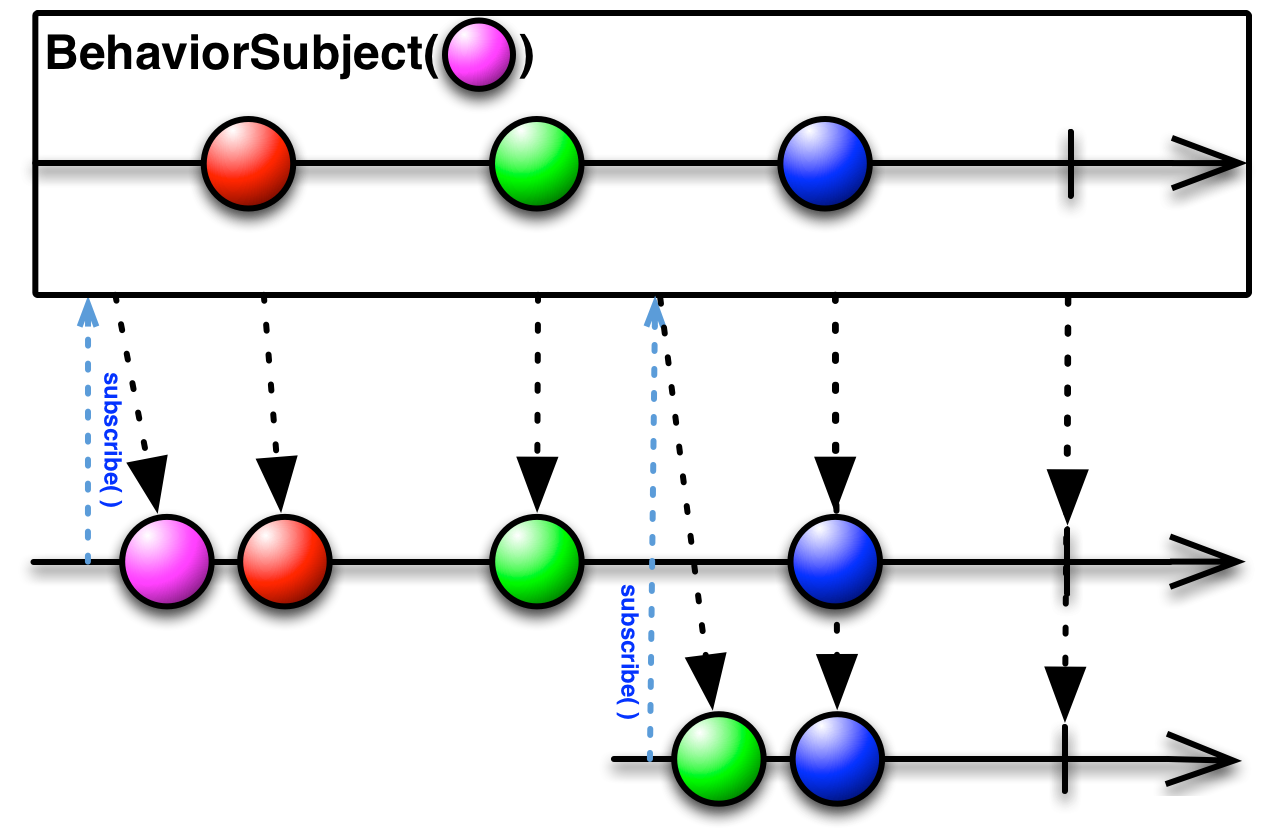
\includegraphics[scale=0.5]{imgs/behasubj.png}
\caption{BehaviorSubject}
\end{figure}

When an observer subscribes to a \texttt{BehaviorSubject}, it begins by
emitting the item most recently emitted by the source Observable (or a
seed/default value if none has yet been emitted) and then continues to
emit any other items emitted later by the source Observable(s).

In practice, it's really similar to the \textbf{Behavior} notion from
Elliot's FRP.

\subsection{RxAndroid}\label{rxandroid}

The previous sections cover all the main topic of RxJava. This section
will go a step further, introducing some additional features that bring
RxJava to the Android ecosystem.

\textbf{RxAndroid} is a separate module of RxJava that gives some
useful bindings to the developer.

The \texttt{AndroidSchedulers} package provides some specific scheduler
for the \emph{Android threading system}.

The additional schedulers provided are:

\begin{itemize}
\itemsep1pt\parskip0pt\parsep0pt
\item
  \texttt{AndroidSchedulers.mainThread(\ )}, that will execute an action
  on the main \textbf{Android UI thread}
\item
  \texttt{AndroidSchedulers.handlerThread(Handler\ handler)}, that
  \textbf{uses the provided Handler} to execute an action
\end{itemize}

A typical example of the usage of \texttt{mainThread(\ )} is the
following, that performs a download in the scheduler \texttt{io(\ )} and
the show the image to the user:

\begin{verbatim}
service.getImage(url)
.subscribeOn(Schedulers.io())
.observeOn(AndroidSchedulers.mainThread())
.subscribe(bitmap -> myImageView.setImageBitmap(bitmap));
\end{verbatim}

\textbf{ViewObservable} is another feature that adds some bindings for
android \texttt{View} that returns observables of events that come from
the UI, such as:

\begin{itemize}
\itemsep1pt\parskip0pt\parsep0pt
\item
  \texttt{clicks(\ )}, that emits a new item each time a \texttt{View}
  is \textbf{clicked}
\item
  \texttt{text(\ )}, that emits a new item each time a
  \texttt{TextView}'s \textbf{text content} is changed
\item
  \texttt{input(\ )}, same as above, for \texttt{CompoundButton}s
\item
  \texttt{itemClicks(\ )}, same as above, for \texttt{AdapterView}s
\end{itemize}

These methods are useful to bind the events from the user of an
application, reifying its action and reacting with some operation, in a
declarative way.

\section{ReactiveCocoa}\label{reactivecocoa}

\textbf{ReactiveCocoa} (RAC) is an opensource framework for FRP,
developed by Github for the \textbf{iOS} and \textbf{OS X} platforms.
RAC has been around for some years now. It started as an
\textbf{Objective-C} framework and now it's object of an almost-complete
rewrite using the brand new language introduced by Apple,
\textbf{Swift}.

At the time of writing (may/june/july 2015), RAC 3.0 is in beta. The 3.0
version offers new APIs in Swift, that are also mostly backward
compatible with version 2.0 (that is written in Objective-C).

Using Swift, the APIs now have a better and cleaner form. In fact, Swift
is a language that allows to build composable abstraction pretty easily,
supporting immutability (value types vs reference types), high-order
functions, optionals, custom operators, etc\ldots{}

In the community of iOS and OS X developers RAC is an emerging trend
that is clearly gaining the attention of an increasing number of users,
confirming the general trend of RP and FRP in our industry.


\subsection{Event and Signal}\label{event-and-signal}

The first abstraction that the framework introduces is the notion of
event. An \textbf{event} enables to account for \emph{discrete
phenomena}, and each of which has a stream (finite or infinite) of
occurrences. Each occurrence is a value paired with a time.
Events are considered to be improving list of occurrences. Or, in simpler
words, events are things that happen.

In RAC, events are first-class citizens, with the following type:

\begin{verbatim}
public enum Event<T, E: ErrorType> {
    case Next(Box<T>)
    case Error(Box<E>)
    case Completed
    case Interrupted
}
\end{verbatim}

The \texttt{Event} type, taken alone, doesn't say much. It's just an
enum with some possible related values.

\begin{quote}
In Swift, an enum is a value type that defines a common type for a group
of related values and enables you to work with those values in a
type-safe way within your code.
\end{quote}

The other fundamental type in RAC is the \texttt{Signal} type, defined
as:

\begin{verbatim}
public final class Signal<T, E: ErrorType>
\end{verbatim}

A signal is just a sequence of events in time that is conforms to the
grammar
\texttt{Next*\ (Error\ \textbar{}\ Completed\ \textbar{}\ Interrupted)?}.
The grammar introduces a precise semantics and clarify the meaning of
the concrete possible instances for the Event type:

\begin{itemize}
\itemsep1pt\parskip0pt\parsep0pt
\item
  \texttt{.Next} represents an event that carry information of a given
  type \texttt{T}
\item
  \texttt{.Error} represents an event that carry an error of a given
  type \texttt{E}
\item
  \texttt{.Completed} represents a successful terminal event
\item
  \texttt{.Interrupted} represents an event that indicates that the
  signal has been interrupted
\end{itemize}

Just like RxJava's Observable, also RAC's signal can be distincted in
two main categories: hot and cold signals. The main difference from
RxJava's implementation is that in RAC this fundamental distinction can
be found directly in the types. In fact, RAC defines \texttt{Signal}as
hot and \texttt{SignalProducer} as cold signals.

\emph{NB}: the previous introduction of Signal is general and applicable
on both Signal and SignalProducer.

The next sections will go deeper and explore more on Signals and
SignalProducers.

\subsubsection{Signal}\label{signal}

As introduced previously, Signal implements the abstraction of
\textbf{hot signal} as a signal that typically has \textbf{no start and
no end}.

A typical practical example for this type can be represented by the press
events of a button or the arrival of some notifications. They are just
events that happens with no relevance of the fact that someone is
observing them.

Using a popular philosophical metaphor:

\begin{quote}
If a tree falls in a forest and no one is around to hear it, \textbf{it
does make a sound}.
\end{quote}

Looking at the documentation, a Signal is defined as a \emph{push-driven
stream that sends Events over time}. Events will be sent to all
observers at the same time. So, if a Signal has different observers
subscribed to its events, every observer will always see the same
sequence of events.

The documentation says another crucial thing that clarifies the
modelling choice made by the developers:

\begin{quote}
Signals are generally used to represent event streams that are already
``in progress'', like notifications, user input, etc. To represent
streams that must first be \emph{started}, see the SignalProducer type.
\end{quote}

The RAC' maintainers decided to keep the distinction between hot and cold
Signal at the type level, so RAC offers both the \texttt{Signal} and
\texttt{SignalProducer} types.

The \texttt{Signal} type is defined as follows:

\begin{verbatim}
class Signal<T, E: ErrorType> {
  ...
}
\end{verbatim}

Signal is parameterized over \texttt{T}, the type of the events emitted
by the signal and \texttt{E}, the type that denotes the errors.

A Signal can be created by passing to the initializer a generator
closure, which is then invoked with a sink of type
\texttt{SinkOf\textless{}Event\textless{}String,\ NoError\textgreater{}\textgreater{}}.
The sink is then used by the closure to forward events to the Signal
through the \texttt{sendNext(\ )} method. A similar approach has been
implemented also by Akka Streams.

\textbf{In many cases, a stream of events that has no start and no end
can't terminate with an error.} A simple example of this case is a
stream of press events from a button. To overcome this possibility, RAC
introduces the type \texttt{NoError}, meaning that the signal can't
error out.

For the ``button example'', the type for the related signal might be
\texttt{Signal\textless{}Void,\ NoError\textgreater{}}, which means:

\begin{itemize}
\itemsep1pt\parskip0pt\parsep0pt
\item
  the user of the signal only cares about the occurrence of the event, no
  further information will be provided
\item
  the signal can't error out, since in this particular case it has no
  sense to model the fact that a button press can fail
\end{itemize}

The button example is just one of many others. If we consider the amount
of events that come from the UI, a lot of trivial examples come out
quickly:

\begin{itemize}
\itemsep1pt\parskip0pt\parsep0pt
\item
  a signal that models the changes of a text field
\item
  a signal that models the arrival of notifications (remote, local,
  etc\ldots{})
\item
  any other signal created combining other signals
\item
  \ldots{}
\end{itemize}

An example for the creation of a Signal is the following, taken from a
blog post of Colin Eberhardt, where a new String is produced every
second.

\begin{verbatim}
func createSignal() -> Signal<String, NoError> {
  var count = 0
  return Signal {
    sink in
    NSTimer.schedule(repeatInterval: 1.0) { timer in
      sendNext(sink, "tick #\(count++)")
    }
    return nil
  }
}
\end{verbatim}

To attach some side effect at each \texttt{Next}, \texttt{Error} or
\texttt{Completed} event that is produced by a \texttt{Signal}, an
observer has to register its interest using \textbf{observe}. The
\texttt{observe} operator accepts some closures or functions for any of
the event types the user of the API is interested in.

The real deal in using Signals is their power in term of declarativeness
when combining Signals with operators to create new Signals to work
with.

In RAC, all \textbf{operations} that can be applied to signals are
simply \textbf{free functions}, in contrast to the
``classical-method-definition-on-the-Signal-type approach''. As an
example, the \texttt{map} operator signature is defined as follows, with
the Signal on which the transformation will be applied passed as an
argument:

\begin{verbatim}
public func map<T, U, E>(transform: T -> U)
    (signal: Signal<T, E>) -> Signal<U, E> {
    ...
}
\end{verbatim}

To keep the APIs fluent RAC also introduces the pipe-forward operator
\texttt{\textbar{}\textgreater{}}, defined as follows:

\begin{verbatim}
public func |> <T, E, X>(signal: Signal<T, E>,
    transform: Signal<T, E> -> X) -> X {
    return transform(signal)
}
\end{verbatim}

The \texttt{\textbar{}\textgreater{}} operator doesn't do anything
special, since it only creates a specification.

RAC already offers a numbers of built in operators as free functions,
such as \texttt{combineLatest}, \texttt{zip}, \texttt{takeUntil},
\texttt{concat}, \ldots{}

A complete but simple example of usage of all of the aspects introduced
is the following:

\begin{verbatim}
createSignal()
  |> map { $0.uppercaseString }
  |> observe(next: { println($0) })
\end{verbatim}

The beauty of this approach is that the chain of operations fits the
types of each operation, so when the code compiles (and if the user of
the APIs has learned the semantics of each operators) the computation
acts as expected. All the relevant work for the newcomers of the
paradigm consist in taking the time needed to learn the basics and play
with the types and the operators.

\subsubsection{SignalProducer}\label{signalproducer}

The previous section introduced \texttt{Signal} as the type that
implements the ``hot signal'' abstraction. This section will cover the
other half of the story.

In RAC, \textbf{``cold signals''} are implemented with the
\texttt{SignalProducer} type, defined as follows:

\begin{verbatim}
public struct SignalProducer<T, E: ErrorType> {
    ...
}
\end{verbatim}

The generic types are the same as its ``hot'' counterpart, and also the
initializer is pretty similar, with a generator closure:

\begin{verbatim}
func createSignalProducer() -> SignalProducer<String, NoError> {
  var count = 0
  return SignalProducer {
    sink, disposable in
    NSTimer.schedule(repeatInterval: 0.1) { timer in
      sendNext(sink, "tick #\(count++)")
    }
  }
}
\end{verbatim}

Using a popular philosophical metaphor, again:

\begin{quote}
If a tree falls in a forest and no one is around to hear it, \textbf{it
doesn't make a sound}.
\end{quote}

Or, in other words, if no one subscribes to the SignalProducer, nothing
happens. For SignalProducer, the terminology for subscribing to its
events is \texttt{start(\ )}.

If more than one observer subscribe to the same SignalProducer, the
resources are allocated for each observer. In the example above, every
time an observer invoke the \texttt{start(\ )} method on the same
SignalProducer instance, a new instance of NSTimer is allocated.

Also on SignalProducers can be applied a wide range of operators. RAC
doesn't implement all the operators twice for Signal and SignalOperator,
but it offers a pipe-forward operator that lifts the operators and
transformation that can be applied to \texttt{Signal} to also operate on
\texttt{SignalProducer}.

The implementation of \texttt{\textbar{}\textgreater{}}, that applies on
the SignalProducer type using Signal's operator, is the following:

\begin{verbatim}
public func |> <T, E, U, F>(producer: SignalProducer<T, E>,
      transform: Signal<T, E> -> Signal<U, F>) -> SignalProducer<U, F> {
  return producer.lift(transform)
}
\end{verbatim}

\subsection{ProperyType}\label{properytype}

The previous sections introduced the abstractions that RAC offers to
describe signal. This section will introduce other collateral but
useful types.

\texttt{PropertyType} is a protocol that, when applied to a property,
\textbf{allows the observation of its changes}. Its definition is as
follows:

\begin{verbatim}
public protocol PropertyType {
    typealias Value

    var value: Value { get }
    var producer: SignalProducer<Value, NoError> { get }
}
\end{verbatim}

The semantics of this protocol is neat: - the \textbf{getter} return the
current value of the property - the \textbf{producer} return a producer
for Signals that will send the property's current value followed by all
changes over time

Starting from this protocol, RAC introduces: -
\texttt{ConstantProperty}, that represents a property that never change
- \texttt{MutableProperty}, that represents a mutable property -
\texttt{PropertyOf}, that represents a read-only view to a property

These types are really usefull when used in combination with the
\texttt{\textless{}\textasciitilde{}} operator, that binds properties
together. The bind operator comes in three flavors:

\begin{verbatim}
/// Binds a signal to a property, updating the property's
/// value to the latest value sent by the signal.
public func <~ <P: MutablePropertyType>(property: P, signal: 
	Signal<P.Value, NoError>) -> Disposable {}

/// Creates a signal from the given producer, which will 
/// be immediately bound to the given property, updating the 
/// property's value to the latest value sent by the signal.
public func <~ <P: MutablePropertyType>(property: P, 
	producer: SignalProducer<P.Value, NoError>) 
		-> Disposable { }

/// Binds `destinationProperty` to the latest values 
/// of `sourceProperty`.
public func <~ <Destination: MutablePropertyType, 
	Source: PropertyType where Source.Value == Destination.Value>
		(destinationProperty: Destination, 
			sourceProperty: Source) -> Disposable { }
\end{verbatim}

What these operators do is to create the wires that link each property
to each others, in a declarative manner. Each property is observable,
through its inner SignalProducer.


\subsection{Action}\label{action}

The last concept that RAC APIs introduce is the notion of
\texttt{Action}.

An action is something that will do some work in the future. An action
will be executed with an input and will return an output or an error.
Its type is generic, and it's exposed as:

\begin{verbatim}
public final class Action<Input, Output, Error: ErrorType>
\end{verbatim}

The constructor of an Action accepts a closure or a function that
creates a SignalProducer for each input, with the type
\texttt{Input\ -\textgreater{}\ SignalProducer\textless{}Output,\ Error\textgreater{})}.

A practical and useful use of Action is in conjunction with
\texttt{CocoaAction}, which is another type that wraps an Action for use
by a GUI control, with key-value observing, or with other Cocoa
bindings.


\section{Akka Streams}\label{akka-streams}

\textbf{Akka Streams} is a library that is developed on top akka actors,
and aims to provide a better tool for building \emph{ephemeral
transformation pipelines}.

Akka actors are used as a building block to build a higher abstraction.
Some of the biggest issues on building systems on untyped actor are the
following:

\begin{itemize}
\itemsep1pt\parskip0pt\parsep0pt
\item
  actors does \textbf{not compose} well
\item
  actors are \textbf{not} completely \textbf{type safe}
\item
  dealing with an high number of actors, with also a complex logic
  behind each behaviors, is really error prone and bring back an evil
  concept: global \textbf{state}.
\end{itemize}

An actor can be seen as a single \emph{unit of consistency}.

From the introduction of the documentation of akka streams:

\begin{quote}
Actors can be seen as dealing with streams as well: they send and
receive series of messages in order to transfer knowledge (or data) from
one place to another. We have found it tedious and error-prone to
implement all the proper measures in order to achieve stable streaming
between actors, since in addition to sending and receiving we also need
to take care to not overflow any buffers or mailboxes in the process.
Another pitfall is that Actor messages can be lost and must be
retransmitted in that case lest the stream have holes on the receiving
side. When dealing with streams of elements of a fixed given type,
Actors also do not currently offer good static guarantees that no wiring
errors are made: type-safety could be improved in this case.
\end{quote}

To overcome these issues, the developers behind Akka started developing
Akka Streams, a set of APIs that offers an intuitive and safe way to
build \textbf{stream processing pipelines}, with a particular attention
to efficiency and bounded resource usage.

Akka Streams is also conform to the Reactive Streams initiative (see the
appendix), and this means that the hard problem of propagating and
reacting to back-pressure has been incorporated in the design of Akka
Streams already, and also that Akka Streams interoperate seamlessly with
all other Reactive Streams implementations.

In Akka Streams, a linear processing pipeline can be expressed using the
following building blocks:

\begin{itemize}
\itemsep1pt\parskip0pt\parsep0pt
\item
  \textbf{Source}: A processing stage with exactly one output, emitting
  data elements whenever downstream processing stages are ready to
  receive them, respecting their demand.
\item
  \textbf{Sink}: A processing stage with exactly one input, signalling
  demand to the upstream and accepting data elements in response, as
  soon as they're produced.
\item
  \textbf{Flow}: A processing stage which has exactly one input and
  output, which connects its upstream and downstreams by transforming
  the data elements flowing through it.
\item
  \textbf{RunnableFlow}: A Flow that has both ends attached to a Source
  and Sink respectively, and is ready to be run().
\end{itemize}

The APIs also offer another core abstraction to build computation
graphs: 

\begin{itemize}
\itemsep1pt\parskip0pt\parsep0pt
\item
  \textbf{Graphs}: A processing stage with multiple flows
connected at a single point.
\end{itemize}

The next sections will depict all the core abstractions introduced here.


\subsection{Source}\label{source}

In Akka Streams, a \textbf{Source} is a set of stream processing steps
that has \textbf{one open output}. In Scala, the \texttt{Source} type is
defined as follows:

\begin{verbatim}
final class Source[Out]
\end{verbatim}

The \texttt{Out} type is the type of the elements the source produces.

It either can be an atomic source or it can comprise any number of
internal sources and transformation that are wired together. Some
examples of the former case is given from the following code, that shows
some of the utility constructor for the \texttt{Source} type.

\begin{verbatim}
// Create a source from an Iterable
Source(List(1, 2, 3))

// Create a source from a Future
Source(Future.successful("Hello Streams!"))

// Create a source from a single element
Source.single("only one element")

// an empty source
Source.empty
\end{verbatim}

An example of the latter case is when a \texttt{Flow} is attached to a
\texttt{Source}, resulting in a composite source, as in the following
example.

\begin{verbatim}
val tweets: Source[Tweet] = Source(...)
val filter: Flow[Tweet, Tweet] = Flow[Tweet].filter(
	t => t.hashtags.contains(hashtag))
val compositeSource: Source[Tweet] = tweets.via(filter)
\end{verbatim}

The \texttt{via(\ )} method transforms a source by appending the given
processing stages, and it's the glue that enables to build composite
sources.


\subsection{Sink}\label{sink}

The dual to the \texttt{Source} type is the \textbf{Sink} type, which
abstracts a set of stream processing steps that has one open input and
an attached output. In Scala the \texttt{Sink} type is defined as
follows:

\begin{verbatim}
final class Sink[In]
\end{verbatim}

The \texttt{In} type is the type of the elements the sink accepts.

It either can be an atomic sink or it can comprise any number of
internal sinks and transformation that are wired together. Some examples
of the former case is given from the following code, that shows some of
the utility constructor for the \texttt{Sink} type.

\begin{verbatim}
// Sink that folds over the stream and returns a Future
// of the final result as its materialized value
Sink.fold[Int, Int](0)(_ + _)

// Sink that returns a Future as its materialized value,
// containing the first element of the stream
Sink.head

// A Sink that consumes a stream without doing 
// anything with the elements
Sink.ignore

// A Sink that executes a side-effecting call for every 
// element of the stream
Sink.foreach[String](println(_))
\end{verbatim}

An example of the latter case is given by a Flow that is prepend to a
Sink to get a new composite sink, as in the following example:

\begin{verbatim}
val sum: Flow[(Long, Tweet), (Long, Tweet)] = 
	Flow[(Long, Tweet)].scan[(Long, Tweet)](0L, EmptyTweet)(
      (state, newValue) => (state._1 + 1L, newValue._2))
val out: Sink[(Long, Tweet)] = Sink.foreach[(Long, Tweet)]({
      case (count, tweet) => println(count + " Current tweet: " 
      	+ tweet.body + " -  " + tweet.author.handle)
    })

val compositeOut: Sink[(Long, Tweet)] = sum.to(out)
\end{verbatim}


\subsection{Flow and RunnableFlow}\label{flow-and-runnableflow}

The previous sections introduced the two ends of a computation. This
section will introduce the \textbf{Flow} abstraction: a processing stage
which has exactly one input and one output. In Scala, the \texttt{Flow}
type is defined as follows.

\begin{verbatim}
class Flow[In, Out]
\end{verbatim}

The \texttt{Out} type is the type of the elements the flow returns and
the \texttt{In} type is the type of the elements the flow accepts.

A \textbf{RunnableFlow} is a flow that has both ends attached to a
source and sink, and represents \emph{a flow that can run}. A trivial
example of \texttt{RunnableFlow} in action is the following:

\begin{verbatim}
val in: Source[Tweet] = Source(...)
val out: Sink[Tweet] = Sink.foreach(println)
val runnableFlow: RunnableFlow = in.to(out)

runnableFlow.run()
\end{verbatim}

As already introduced, Akka Streams implements an \emph{asynchronous
non-blocking back-pressure protocol} standardised by the Reactive
Streams specification, and the user doesn't have to manually manage
back-pressure handling code manually since this is already provided by
the library itself with a default implementation.

In this regards, there are two main scenarios: \textbf{slow publisher
with fast subscriber} and \textbf{fast publisher with slow subscriber}.

The best scenario is the former, where all the items produced by the
publisher are always delivered to the subscriber with no delay due to a
lack of demand. In fact, the protocol guarantees that the publisher will
never signal more items than the signalled demand, and since the
subscriber however is currently faster, it will be signalling demand at
a higher rate, so the publisher should not ever have to wait in
publishing its items. This scenario is also referred as \emph{push
mode}, since the publisher is never delayed in pushing items to the
subscriber.

The latter case if more problematic, since the subscriber is not able to
keep the pace of the publisher in accepting incoming items and needs to
signal its lack of demand to the publisher. Since the protocol
guarantees that the publisher will never signal more items than the
signalled demand, there the following strategies available:

\begin{itemize}
\itemsep1pt\parskip0pt\parsep0pt
\item
  not generate items, if it can control its production
\item
  buffering the items within a bounded queue, so the items can be
  provided when more demand is signalled
\item
  drop items until more demand is signalled
\item
  as an ultimate strategy, tear down the stream if none of the previous
  strategies are applicable
\end{itemize}

This latter scenario is also referred as \emph{pull mode}, since the
subriber drives the flow of items.

\subsection{Graph}\label{graph}

Since not every computation is or can be expressed as a linear
processing stage pipeline, Akka Streams also provide a graph-resembling
DSL for building stream processing graphs, in which each node can has
multiple inputs and outputs.

The documentation refers to graph operation as \textbf{junctions}, in
which multiple flows are connected at a single point, enabling to
perform any kind of \emph{fan-in} or \emph{fan-out}.

The Flow graph APIs provide a pretty straight forward abstraction:

\begin{itemize}
\itemsep1pt\parskip0pt\parsep0pt
\item
  \textbf{Flow}s represent the \textbf{connection} within the
  computation graph
\item
  \textbf{Junction}s represent the \textbf{fan-in and fan-out} point to
  which the flows are connected
\end{itemize}

The APIs already provide some of the most useful juctions, like the
following:

\begin{itemize}
\itemsep1pt\parskip0pt\parsep0pt
\item
  \texttt{Merge{[}In{]}} - \emph{(N inputs , 1 output)} picks randomly
  from inputs pushing them one by one to its output
\item
  \texttt{Zip{[}A,B{]}} -- \emph{(2 inputs, 1 output)} is a ZipWith
  specialised to zipping input streams of A and B into an (A,B) tuple
  stream
\item
  \texttt{Concat{[}A{]}} -- \emph{(2 inputs, 1 output)} concatenates two
  streams (first consume one, then the second one)
\item
  \texttt{Merge{[}In{]}} -- \emph{(N inputs , 1 output)} picks randomly
  from inputs pushing them one by one to its output
\item
  \texttt{Broadcast{[}T{]}} -- \emph{(1 input, N outputs)} given an
  input element emits to each output
\end{itemize}

The documentation also provide a simple but brilliant example that
illustrates how the DSL provided by the library can be used to express
graph computation keeping a great level of declarativeness and code
readability.

The following image shows a graph that expresses a computation in which:

\begin{itemize}
\itemsep1pt\parskip0pt\parsep0pt
\item
  \textbf{the edges are flows}
\item
  \textbf{the nodes are a sink, a source and two junctions}
\end{itemize}

\begin{figure}[htbp]
\centering
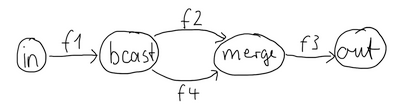
\includegraphics[scale=0.75]{imgs/graph.png}
\caption{A handwritten graph expressing a computation}
\end{figure}

The corresponding computation can be implemented as follows:

\begin{verbatim}
val g = FlowGraph.closed() { 
	implicit builder: FlowGraph.Builder[Unit] =>
  import FlowGraph.Implicits._
  val in = Source(1 to 10)
  val out = Sink.ignore
  val bcast = builder.add(Broadcast[Int](2))
  val merge = builder.add(Merge[Int](2))
  val f1, f2, f3, f4 = Flow[Int].map(_ + 10)
  in ~> f1 ~> bcast ~> f2 ~> merge ~> f3 ~> out
              bcast ~> f4 ~> merge
}
\end{verbatim}

When building and connecting each component, the compiler will check for
type correctness and this is a really useful things. The check to
control whether or not all elements have been properly connected is done
at run-time, though.

The framework also provides the notion of partial graph. A
\textbf{partial graph} is a graph with \emph{undefined sources, sinks or
both}, and it's useful to structure the code in different components,
that will be then connected with other components. In other words, the
usage of partial graphs favours code \textbf{composability}.

In many cases it's also possible to expose a complex graph as a simpler
structure, such as a Source, Sink or Flow, since these concepts can be
viewed as special cases of a partially connected graph:

\begin{itemize}
\itemsep1pt\parskip0pt\parsep0pt
\item
  a source is a partial flow graph with exactly one output
\item
  a sink is a partial flow graph with exactly one input
\item
  a Flow is a partial flow graph with exactly one input and exactly one
  output
\end{itemize}

One last feature that this section will depict and that Akka Stream
supports is the possibility to insert \textbf{cycles} in flow graphs.
This feature is potentially dangerous, since it may lead to deadlock or
liveness issues.

The problems quickly arise when there're unbalanced feedback loops in
the graph. Since Akka Stream is based on processing items in a bounded
manner, if a cycle has an unbounded number of items (for example, when
items always get reinjected in the cycle), the back-pressure will
deadlock the graph very quickly.

A possible strategy to avoid deadlocks in presence of \textbf{unbalanced
cycles} is introducing a \textbf{dropping element on the feedback arc},
that will drop items when back-pressure begins to act.

A brilliant example from the documentation is the following, where a
\texttt{buffer(\ )} is used with a 10 items capacity and a
\texttt{dropHead} strategy.

\begin{verbatim}
FlowGraph.closed() { implicit b =>
  import FlowGraph.Implicits._
  val merge = b.add(Merge[Int](2))
  val bcast = b.add(Broadcast[Int](2))

  source ~> merge ~> Flow[Int].map { 
			s => println(s); s } ~> bcast ~> Sink.ignore
      merge <~ Flow[Int].buffer(10, OverflowStrategy.dropHead) <~ bcast
}
\end{verbatim}

An alternative approach in solving the problem is by \textbf{building a
cycle that is balanced from the beginning}, by using \textbf{junctions
that balance the inputs}. Thus, the previous example can also be solved
in the following manner, with:

\begin{itemize}
\itemsep1pt\parskip0pt\parsep0pt
\item
  a \texttt{ZipWith(\ )} junction, that will balance the feedback loop
  with the source
\item
  a \texttt{Concat(\ )} combined with another \texttt{Source(\ )} with
  an initial element that performs an initial ``kick-off''. In fact,
  using a balancing operator to balance a feedback loops require an
  initial element in the feedback loop, otherwise we fall in the
  ``chicken-and-egg'' problem.
\end{itemize}

\begin{verbatim}
FlowGraph.closed() { implicit b =>
  import FlowGraph.Implicits._
  val zip = b.add(ZipWith((left: Int, right: Int) => left))
  val bcast = b.add(Broadcast[Int](2))
  val concat = b.add(Concat[Int]())
  val start = Source.single(0)

  source ~> zip.in0
  zip.out.map { s => println(s); s } ~> bcast ~> Sink.ignore
  zip.in1 <~ concat <~ start
             concat         <~          bcast
}
\end{verbatim}

\chapter{Towards reactive mobile application development}\label{towards-reactive-mobile-application-development}

The first chapter introduced the literature and the main concepts of the
RP paradigm, and the second one depicted some of the main popular and
used libraries and framework for RP. This chapter will propose a
concrete applications of the paradigm to some pratical use cases that
recur pretty frequently when developpig mobile application nowadays.

Thus, this chapter will focus its attention on mobile application
development, in both the Android and iOS platforms.

The main idea that brings RP to mobile application development is in the
abstraction that considers an app as a function, or as a flow of user
inputs that are continuously evaluated, filtered, combined, and so on,
producing a some sort of outputs and effects.


\section{Abstracting the retrieval, manipulation and presentation of
data}\label{abstracting-the-retrieval-manipulation-and-presentation-of-data}

The first use case proposed is about a quite common set of actions, such
as the \textbf{retrieval, manipulation and presentation of some sort of
data}.

Every simple or complex application has at least a part in the app
lifecycle in which it queries some provider (a cache, a local database,
a Rest API) to fetch some resource, so this initial use case can be
considered as a foundational building block for every application.

The abstraction of event streams can be used to model this use case in a
pretty straigh-forward way.

In the case of a web request, the stream will either emit one value -
containing the body of the response - and succed, or fail with an error.

In the case of more complex request-response configuration (e.g.~a
request that opens a web socket, that then emits and push new data over
a long time) the stream will emit more values, as long as the flow of
items continues, or terminate if a failure occurs.

Abstracting the reception of items is only the first part of the
scenario introduced. Once the application got some kind of data, a
certain number of processing stages can be run over these data. Thus,
the notion of event streams and operators fits really nicely also on
this part.

To demostrate a possible solution of this scenario using an approach
based on RP, lets introduce a sample use case:

\begin{quote}
The application has to query a web service, that returns a list of words
for a given month. Each word refers to a specific day, month and year.
The application should show all the words in the given month, sorted by
date, with the first one highlighted with a different color.
\end{quote}

\subsection{On Android}\label{on-android}

After introducing the use case, the first thing to do is to write down
the types involved in the computation and to provide a class that
handles the network requests, returning an observable with the response.
This class will be part of the network layer of the application, and
will expose methods like the following:

\begin{verbatim}
public Observable<List<Word>> getWords(int month, int year);
\end{verbatim}

As a reference, the \texttt{Word} type is the following:

\begin{verbatim}
public class Word {
    public long id;
    public String word;
    public int day;
    public int month;
    public int year;
}
\end{verbatim}

The semantics for this observable is pretty simple:

\begin{itemize}
\itemsep1pt\parskip0pt\parsep0pt
\item
  it \emph{yields} a single results (the response body) or an error (a
  network error, or a server error, etc..)
\item
  it \emph{starts} the computation each times a consumer
  \emph{subscribes} itself to the observable
\end{itemize}

NB: for this kind of request, the behavior would also have been
implemented with a future.

Once the network layer is in place, all the transformation needed can be
expressed in term of operators.

\begin{verbatim}
myServiceProvider.getWords(month, year)

    // network operations in io scheduler
    .subscribeOn(Schedulers.io())

    // Observable<List<Word>> -> Observable<Word>
    .flatMap(wordList -> Observable.from(wordList))

    // sort elements
    .toSortedList((l, r) -> { ...sort predicate... })

    // Observable<List<Word>> -> Observable<Word>
    .flatMap(list -> Observable.from(list))

    // build an Observable<Pair<Integer, Word>> 
    // (the integer value is the index)
    .map(word -> new Pair<>(0, word))
    .scan((sum, item) -> new Pair<>(sum.first + 1, item.second))

    // build list adapter, highlighting the first element
    // Observable<Pair<Integer, Word>> -> Observable<WordListItem>
    .map(indexItemPair -> { 
        WordListAdapter.WordListItem item 
        	= new WordListAdapter.WordListItem(indexItemPair.second);
        item.setHighlighted(...); // highlight current day item
        return item;
    })
    .toList() // converting to list, since the adapter need a list

    //  UI update on main thread
    .observeOn(AndroidSchedulers.mainThread())

    // subscribing to items, errors, ...
    .subscribe(
        wordItemList -> {
            setListAdapter(
            	new WordListAdapter(wordListActivity, wordItemList));
        },
        throwable -> {
        ...
        }
    );
\end{verbatim}

The code shows some transformations and some usage of the most common
operators of RxJava.

In the code snippet, \texttt{flatMap} is used to transform an
\texttt{Observable\textless{}List\textless{}Word\textgreater{}\textgreater{}}
to an \texttt{Observable\textless{}Word\textgreater{}}. This is a pretty
common transformation when dealing with list of elements, and since
operators like \texttt{map}, \texttt{filter}, etc.. need to operate on
single elements, this operation is essential to build the chain.

Another pattern is the usage of \texttt{map} in conjuction with
\texttt{scan}, to accumulate the result of a computation. The code
presented does the trivial job of associating to each element its index
in the observable, but it's a use case useful enought to deserve a
citation.

The presentation of the items is provided by the
\texttt{WordListAdapter} and \texttt{WordListItem} classes.

One last things to note is the usage of \texttt{subscribeOn} and
\texttt{observeOn}, to keep the main thread responsive.

\subsection{On iOS}\label{on-ios}

On iOS, the problem can be solved using the same conceptual
abstractions.

Starting with a network provider that expose the call to the APIs with
the following method signature:

\begin{verbatim}
func getWords(month: Int, year: Int) -> SignalProducer<[Word], NSError>
\end{verbatim}

As a reference, the type \texttt{Word} is defined as follows:

\begin{verbatim}
public struct Word {

    public let id: Int
    public let word: String
    public let day: Int
    public let month: Int
    public let year: Int

    init(id: Int, word: String, day: Int, month: Int, year: Int){
        self.id = id
        self.word = word
        self.day = day
        self.month = month
        self.year = year
    }
}
\end{verbatim}

Also on iOS, the semantics for this signal producer is pretty simple and
similar to the androd counterpart:

\begin{itemize}
\itemsep1pt\parskip0pt\parsep0pt
\item
  it \emph{yields} a single results (the response body) or an error (a
  network error, or a server error, etc..)
\item
  it \emph{starts} the computation each times a consumer
  \emph{subscribes} itself on the signal producer
\end{itemize}

\begin{verbatim}
getWords(month, year)
    // sort
    |> map { words in words.sorted(...) }

    // SignalProducer<[Word]> -> SignalProducer<Word>
    |> flatMap(FlattenStrategy.Merge, { 
    	words in SignalProducer(values: words) })

    // build an SignalProducer<(Int, Word)>
    // (the integer value is the index)
    |> map { word in (0, word) }
    |> scan( (0, nil), { (last, current) in (last.0 + 1, current.1) })

    // observe on UI thread
    |> observeOn(UIScheduler())

    // start and subscribe to elements, errors, ...
    |> start(next: { elem in self.updateView(elem)})
\end{verbatim}

Almost every step of the chain is the same as its android conunterpart.
The main difference is that RAC doesn't offer a method to sort the
elements of a SignalProducer, so, in this case, the elements are
filtered at the beginning of the chain using a method of the
\texttt{Array} type.


\section{Choosing an architectural
pattern}\label{choosing-an-architectural-pattern}

This section will explore a foundamental aspect of mobile application
development: the architectural pattern.

When developping a mobile applications, usually the target platform
implicitely or explicitely suggests an architecture.

\subsection{State of the art in iOS}\label{state-of-the-art-in-ios}

In the iOS world, Apple encourages the usage of the
Model-View-Controller (MVC) architectural pattern. Quoting the ``Start
Developing iOS Apps Today'' Apple's documentation:

\begin{quote}
\textbf{MVC} assigns the objects in an app to one of three roles:
\textbf{model}, \textbf{view}, or \textbf{controller}. In this pattern,
models \emph{keep track} of your app's data, views \emph{display} your
user interface and \emph{make up the content} of an app, and controllers
\emph{manage} your views. By responding to user actions and populating
views with content from the data model, controllers serve as a
\emph{gateway} for communication between the model and views.
\end{quote}

\begin{figure}[htbp]
\centering
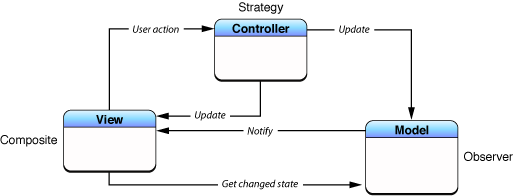
\includegraphics[scale=0.75]{imgs/ios_traditional_mvc.png}
\caption{Traditional MVC in iOS}
\end{figure}

In its original abstraction, in MVC:

\begin{itemize}
\itemsep1pt\parskip0pt\parsep0pt
\item
  the user manipulates a view and, as a result, an event is generated
\item
  a controller receives the event and manage apply an
  appliction-specific strategy
\item
  this strategy can consist in requesting a model object to update its
  state or in requesting a view object to change its appearance.
\item
  the model object notifies all objects who have registered as observers
  when its state changes; if the observer is a view object, it may
  update its appearance accordingly.
\end{itemize}

\begin{figure}[htbp]
\centering
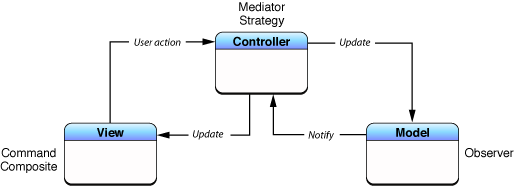
\includegraphics[scale=0.75]{imgs/cocoa_mvc.png}
\caption{Cocoa version of MVC}
\end{figure}

However, in an attempt to enhance code reusability, Apple suggests
developers to adopt a modified version of MVC, in which there's a strong
isolation from models and views, and in which controllers act an
intermediary between one or more of an application's view objects and
one or more of its model objects.

Even if views and view controllers are technically distinct components
and Apple suggests to keep these decoupled, they are almost always
paired. There are a lot reason that cause this trend of strictly
coupling a view and its controller:

\begin{itemize}
\itemsep1pt\parskip0pt\parsep0pt
\item
  the framework provides a big set of components in which a controller
  already has and manages a view (\texttt{UIViewController},
  \texttt{UITableViewController}, \texttt{UICollectionViewController},
  \texttt{UISplitViewController}, \texttt{TabBarController}, \ldots{})
\item
  the UIViewController class usually contains a lot of UI-related code
\item
  storyboards, that enable developers or designers to define GUIs,
  reason in term of view controllers and ``segue'' between view
  controllers
\end{itemize}

With this said, it is reasonable to modify the previous model with an
update in which the view and the view controller are paired togheter.

\begin{figure}[htbp]
\centering
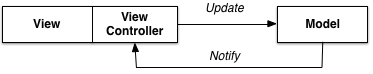
\includegraphics[scale=0.75]{imgs/real_mvc.png}
\caption{A revised iOS application architecture, in which the view and
the controller are coupled}
\end{figure}

The iOS community, during the years, has adopted (also unconsciously)
this architectural pattern to design applications. This has often lead
to what is called the ``Massive View Controller'' anti-pattern. The term
``Massive'' is used to denote the use and abuse of the view controller
entity to host most of the application logic, grouping functionalities
that don't stricly relate to the controller entity.

\subsection{State of the art in
Android}\label{state-of-the-art-in-android}

Android's documentation is less explicit about the architectural pattern
that developers should use.

At first sight, the overall architecture looks similar at iOS's
architecture, with the notion of \texttt{Activity} that is similar to
\texttt{UIViewController} and the notion of \texttt{View} that is
similar to \texttt{UIView}.

But, more in depth, things are far more complicated. Thus, the main flaw
comes from the assumption that there should be only one running
\texttt{Activity} at a time, and that this \texttt{Activity} should be
tied down to a single main view. To overcome this limitation, Android
introduced the \texttt{Fragment} class. This new abstraction allows an
activity to show and manage a certain number of fragments, but still has
some limitations like, for example, the possibility of manage stack of
fragments.

From this point of view, the iOS platform offers a clearer abstractions,
with the notion of viewcontrollers, views and viewcontroller containers,
that allow the developer to express multi-level view hierarchy in a
cleaner way.

Many developers suggest that what Android is offering is a broken
abstraction.

Knowing the limitations of the abstractions that the platform offers,
the most popular architectural pattern for Android is a variant of MVC
(similar to Apple's variant), in which the \texttt{Activity} (and
related fragments) is both a the view and the controller. Google
encourages developers to split each view in a fragment, and then each
fragment should interact with its parent activity, also to coordinate
his actions and commands with other fragments.

\subsection{Toward a common architecture:
MVVM}\label{toward-a-common-architecture-mvvm}

On both the platforms, the MVC architectural pattern and its variations
doesn't seem to be a perfect fit.

In this section and in the following ones a new architectural pattern
will be proposed to better model mobile applications: the
\textbf{Model-View-ViewModel} pattern.

The reason of the introduction of MVVM in this thesis is that this
pattern is an application pattern that isolates the user interface from
the underlying business logic, and, as introduced in the previous
section, one of the biggest issue of the usage of the MVC pattern is the
fact that in both Android and iOS there's not a clear distinction
between the view and the controller entities.

The MVVM pattern consists of the following parts:

\begin{itemize}
\itemsep1pt\parskip0pt\parsep0pt
\item
  the \textbf{Model}, which provides a view-independent representation
  of business entities;
\item
  the \textbf{View}, which is the user interface, displaying information
  to the user and firing events in response to user interactions;
\item
  the \textbf{ViewModel}, which is the bridge between the view and the
  model. Each View has at least a corresponding ViewModel. The ViewModel
  retrieves data from the Model and manipulates it into the format
  required by the View, wrapping the presentation logic. It notifies the
  View if the underlying data in the model is changed, and it updates
  the data in the Model in response to UI events from the View.
\end{itemize}

\begin{figure}[htbp]
\centering
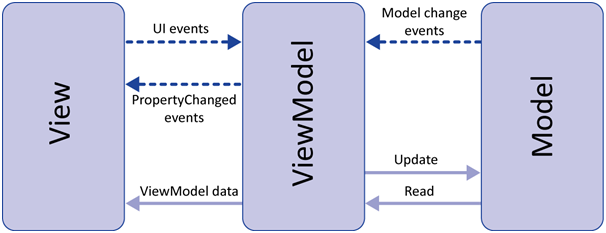
\includegraphics[scale=0.75]{imgs/mvvm.png}
\caption{The MVVM architecural pattern}
\end{figure}

Looking at the diagram, it's clear that the view-model:

\begin{itemize}
\itemsep1pt\parskip0pt\parsep0pt
\item
  sits between the model and the view, \textbf{wrapping all the
  presentation logic}
\item
  receives the events and commands from the view
\item
  \textbf{updates the view} once the model has been updated
\end{itemize}

The main reason to use MVVM is the it \textbf{reduces the complexity} of
one's viewcontrollers or activities and makes one's presentation logic
easier to test.

RP frameworks are a good fit in MVVM, since they allow to \textbf{bind
the views with their associated view-models}, allowing the proper
\textbf{synchronization} to reflect the changes in both directions.

\section{A case study}\label{a-case-study}

To illustrate the application of the MVVM pattern in conjuction with RP
frameworks, let's introduce a simple-but-effective use case.

The use case is an app for iOS and Android, that will:

\begin{itemize}
\itemsep1pt\parskip0pt\parsep0pt
\item
  fetch a web service to request a list of words;
\item
  each words has a set of attributes, such as: an id, a title, a day, a
  month and a year which is related to, and an url to an image;
\item
  after querying the web service, the result should be showed in a list.
  Each list item should display all the attributes, with also the image;
\item
  a detail view should be opened when the user taps on an item.
\end{itemize}

The requirements are pretty trivial for an experienced developer that
use to work following the ``standard'' way to develop mobile
applications, but in this thesis author's hopinion is a pretty
significative example, since it allows to demostrate a lot of concepts:

\begin{itemize}
\itemsep1pt\parskip0pt\parsep0pt
\item
  abstracting the retrieval, manipulation and presentation of data (also
  see the previous dedicated section);
\item
  presenting an uniform abstraction, applyable on both the platforms;
\item
  proper separation of concerns, applying MVVM.
\end{itemize}


\subsection{A common architecture}\label{a-common-architecture}

Starting from the requirements and with \textbf{MVVM} in mind, what
follows is the proposed overall system architecure.

\begin{figure}[htbp]
\centering
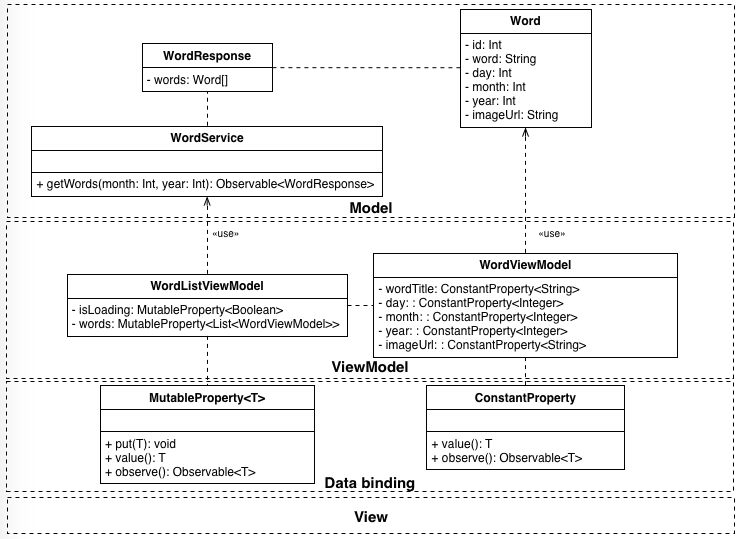
\includegraphics[scale=0.5]{imgs/common_arch.png}
\caption{The overall architecture}
\end{figure}

NB: the diagram is incomplete, and shows only the relevant building
block of the system. The convention used here to express the abstraction
of stream of items is the RxJava's \texttt{Observable} type.

What immediately emerges looking at the digram is how the MVVM pattern
is applied to model the requirements.

The \textbf{Model} provides a view-independent representation of the
business entities. In this case, it's pretty trivial to express the
model of the Word class.

The \textbf{View} doesn't show something relevant at this stage, since
it heavily depends on platform-specific abstractions, and for this
reason it will be better depicted in the next two sections.

The \textbf{ViewModel} is the bridge between the view and the model,
wrapping all the presentation logic. In particular, there're two
concrete type of viewmodels:

\begin{itemize}
\itemsep1pt\parskip0pt\parsep0pt
\item
  \texttt{WordListViewModel}, that represent the viewmodel for the list
  view, as a whole;
\item
  \texttt{WordViewModel}, that represent the viewmodel for a single item
  of the list.
\end{itemize}

\texttt{WordListViewModel} use a \texttt{WordService}, that is a class
that wraps all the network and parsing operations, returning a
\texttt{WordResponse}, that contains an array of \texttt{Word}.
\texttt{WordListViewModel} has two \texttt{MutableProperty}:

\begin{itemize}
\itemsep1pt\parskip0pt\parsep0pt
\item
  \texttt{isLoading}, that indicates if there's a fetch request running
\item
  \texttt{words}, that contains the updated list of words
\end{itemize}

\texttt{WordViewModel} is a pretty simple entity, only containing some
\texttt{ConstantProperty}, referring to the word attributes. The number
of instances of \texttt{WordViewModel} will be equal to the number of
\texttt{Word} returned by the \texttt{WordService}.

\texttt{MutableProperty} and \texttt{ConstantProperty} are two
abstractions that help in binding the viewmodel to the view, allowing to
set up the automatic update of the view layer when the model gets
updated.

Note that this architecture is platform-agnostic and there're no
reference to a specific platform or native abstractions, except for the
\texttt{Observable} type (which can be easily traduced in
\texttt{SignalProducer}, in this specific context).

\subsubsection{Is this RP?}\label{is-this-rp}

Looking at the whole architecture, a question may arise. Is this RP?

The answer to this question is not trivial, at first glance. In the
introduced architecture RP abstraction are used as building block to
compose the overall architecture.

For example, the \texttt{WordService} class returns an
\texttt{Observable}. This immediately suggests a whole set of
considerations about the underlying computation.

Another example are the \texttt{MutableProperty} and
\texttt{ConstantProperty} classes, that under the hood are implemented
as \texttt{Subject} (or \texttt{Signal/SignalProducer}).

In conclusion, RP abstractions can be used as means to properly build
the overall architecture.


\subsection{Implementation on Android}\label{implementation-on-android}

The previous section proposed an overall architecture for the use case.
This sections will depict a possible implementation for the Android
platform.

\subsubsection{Model}\label{model}

Starting from the \textbf{model}, things are pretty straightforward.

The \texttt{Word} type only contains some read-only properties and a
constructor.

\begin{verbatim}
public class Word {

    public final long id;
    public final String word;
    public final int day;
    public final int month;
    public final int year;
    public final String imageUrl;

    public Word(int id, String word, int day,
        int month, int year, String imageUrl) {

        this.id = id;
        this.word = word;
        this.day = day;
        this.month = month;
        this.year = year;
        this.imageUrl = imageUrl;
    }
}
\end{verbatim}

The \texttt{WordResponse} class only wraps an array of \texttt{Word},
and also the logic for failed requests (that is omitted for the sake of
concisness).

\begin{verbatim}
public class WordResponse {
    final public Word[] words;
    WordResponse(Word[] words) {
        this.words = words;
    }
}
\end{verbatim}

Finally, the \texttt{WordService} class only expose a public method that
returns an \texttt{Observable\textless{}WordResponse\textgreater{}}.
Also in this case, the real implementation of this method is not
important for the purpose of this thesis, and it's omitted. The real
important thing of this class is the return type of the method
signature.

\begin{verbatim}
public class WordService {
    public WordService() { ... }
    public Observable<WordResponse>
        getWords(int month, int year) {
        ...
    }
}
\end{verbatim}

\subsubsection{Data binding}\label{data-binding}

To better understand the following steps, it's necessary to introduce
the abstraction of \texttt{MutableProperty} and
\texttt{ConstantProperty}. On the iOS conterpart, ReactiveCocoa already
offers the corresponding abstraction. RxJava and RxAndroid don't
directly offer the conceptual equivalent, but it's pretty easy to build
the same abstraction starting from a \texttt{BehaviorSubject}.

\begin{verbatim}
public interface Val<T> {
    T value();

    boolean hasValue();

    Observable<T> observe();
}
\end{verbatim}

The \texttt{Val} interface introduces the notion of a \textbf{value} of
type \texttt{T}.

\begin{verbatim}
public interface Var<T> extends Val<T> {
    void put(T value);
}
\end{verbatim}

The \texttt{Var} interface introduces a \textbf{variable} of a type
\texttt{T}.

\begin{verbatim}
public class MutableProperty<T> implements Var<T> {
    private final BehaviorSubject<T> subject;
    private Val<T> val;

    protected MutableProperty() {
        subject = BehaviorSubject.create();
    }

    protected MutableProperty(T defaultValue) {
        subject = BehaviorSubject.create(defaultValue);
    }

    public static <T> MutableProperty<T> create() {
        return new MutableProperty<>();
    }

    public static <T> MutableProperty<T> create(T defaultValue) {
        return new MutableProperty<>(defaultValue);
    }

    @Override public void put(T value) {
        subject.onNext(value);
    }

    @Override public synchronized Val<T> asVal() {
        if (val == null) {
            val = ConstantProperty.of(this);
        }

        return val;
    }

    @Override public T value() {
        return subject.getValue();
    }

    @Override public boolean hasValue() {
        return subject.hasValue();
    }

    @Override public Observable<T> observe() {
        return subject.asObservable();
    }
}
\end{verbatim}

The \texttt{MutableProperty} implements the \texttt{Var} interface, and
represents the abstraction of a property that is \textbf{updated over
the time}. This kind of property has a notion of current value (that can
also be absent) and can be observed, returning an \texttt{Observable}.

\begin{verbatim}
public class ConstantProperty<T> implements Val<T> {
    private final Var<T> var;

    protected ConstantProperty(Var<T> var) {
        this.var = var;
    }

    public static <T> ConstantProperty<T> of(Var<T> var) {
        return new ConstantProperty<>(var);
    }

    public static <T> ConstantProperty<T> create(T val) {
        return ConstantProperty.of(new MutableProperty(val));
    }

    @Override public T value() {
        return var.value();
    }

    @Override public boolean hasValue() {
        return var.hasValue();
    }

    @Override public Observable<T> observe() {
        return var.observe();
    }
}
\end{verbatim}

The \texttt{ConstantProperty} implement a property that can have a
single-assignment (constant) value.

\subsubsection{ViewModel}\label{viewmodel}

Moving to the viewmodel layer, things starts to become interesting.

\begin{verbatim}
public class WordListViewModel {

    private static final String TAG 
    	= WordListViewModel.class.getSimpleName();

    public final MutableProperty<Boolean> isLoading =
        MutableProperty.create(false);
    public final MutableProperty<List<WordViewModel>> words =
        MutableProperty.create(new LinkedList<>());

    public WordListViewModel(WordService wordService) {

        wordService.getWords(1, 2015)
                .doOnSubscribe(() -> this.isLoading.put(true))
                .observeOn(AndroidSchedulers.mainThread())
                .flatMap(wordResponse ->
                    Observable.from(wordResponse.words))
                .map(word -> new WordViewModel(word))
                .toList()
                .subscribe(wordViewModelList -> {
                            this.isLoading.put(false);
                            this.words.put(wordViewModelList);
                        },
                        throwable -> {
                            this.isLoading.put(false);
                            Log.e(TAG, throwable.getMessage());
                        });
    }
}
\end{verbatim}

As previously introduced in the architecture diagram, the
\texttt{WordListViewModel} class has two public
\texttt{MutableProperties} and exposes a constructor that receives a
\texttt{WordService}.

When an instance of \texttt{WordListViewModel} is created, the viewmodel
provides to build the chain of computations needed to perform its job.
In this case, it starts a fetch request using the \texttt{WordService}
instance, and then setting all the proper side-effects.

If everything completes fine, the two mutable properties are updated as
follows:

\begin{itemize}
\itemsep1pt\parskip0pt\parsep0pt
\item
  in \texttt{isLoading} is put \texttt{false}, so any view that observe
  that property will be notified of the termination of the request
\item
  in \texttt{words} is put a List
\end{itemize}

\begin{verbatim}
public class WordViewModel {

    final public ConstantProperty<String> wordTitle;
    final public ConstantProperty<Integer> day;
    final public ConstantProperty<Integer> month;
    final public ConstantProperty<Integer> year;
    final public ConstantProperty<String> imageUrl;

    public WordViewModel(Word word) {
        this.wordTitle = ConstantProperty.create(word.word);
        this.day = ConstantProperty.create(word.day);
        this.month = ConstantProperty.create(word.month);
        this.year = ConstantProperty.create(word.year);
        this.imageUrl = ConstantProperty.create(word.imageUrl);
    }
}
\end{verbatim}

The \texttt{WordViewModel} class is even simpler, since it only contains
a set of \texttt{ConstantProperty}, abstracting the set of attributes of
the \texttt{Word} class.

\subsubsection{View}\label{view}

The view layer is represented by three main components:

\begin{itemize}
\itemsep1pt\parskip0pt\parsep0pt
\item
  an \texttt{Activity}, named \texttt{MainActivity}
\item
  a \texttt{Fragment}, named \texttt{MainActivityFragment}, that is
  contained in the \texttt{MainActivity}
\item
  a RecyclerView.Adapter, named \texttt{WordListAdapter}, that is
  necessary to implement a list view in Android
\end{itemize}

The \texttt{MainActivity}'s only job is to instatiate a
\texttt{MainActivityFragment}, so its code is omitted.

\begin{verbatim}
public class MainActivityFragment extends Fragment {
    private RecyclerView mRecyclerView;
    private ProgressBar mProgressBar;
    private WordListAdapter mAdapter;

    ...

    @Override public void onResume() {
        super.onResume();

        if (mRecyclerView.getAdapter() != null) return; 
        final WordService wordService = new WordService();
        final WordListViewModel wordListViewModel 
        	= new WordListViewModel(wordService);

        // bind ui to current loading status
        wordListViewModel.isLoading.observe()
                .observeOn(AndroidSchedulers.mainThread())
                .subscribe(ViewActions.setVisibility(mProgressBar));

        // bind the adapter view with the view model
        mAdapter = new WordListAdapter(wordListViewModel.words.observe());
        mRecyclerView.setAdapter(mAdapter);

        // observe selection event and 
        // show another view with the selected content
        mAdapter.getSelectedWordViewModelObservable()
                .observeOn(AndroidSchedulers.mainThread())
                .subscribe(selectedWordViewModel ->
                        Toast.makeText(getActivity(),
                        selectedWordViewModel.wordTitle.value(), 
                        	Toast.LENGTH_SHORT).show());
    }
}
\end{verbatim}

\texttt{MainActivityFragment} is a really crucial point of the
application. In this class is created a \texttt{WordService}, that is
then passed to a newly created \texttt{WordListViewModel}.

The fragment then binds the viewmodel's properties:

\begin{itemize}
\itemsep1pt\parskip0pt\parsep0pt
\item
  to set the visibility of a progress bar;
\item
  to show the list of items, through an adapter.
\end{itemize}

The last things that the fragment performs is to register its interest
in the item selection events from the adapter. In this simple use case,
the fragment just shows a message in a \texttt{Toast}, but in more real
use case scenario this can be the entry point for a fragment transaction
or for the launch of a new activity.

\begin{verbatim}
public class WordListAdapter
    extends RecyclerView.Adapter<WordListAdapter.WordViewHolder> {

    private List<WordViewModel> mViewModels = new LinkedList<>();
    private PublishSubject<WordViewModel> mAdapterSelectedItemSubject;

    /**
     * Constructor that returns a WordListAdapter, with an observable
     * containing a list of view models
     *
     * @param viewModelsObservable an observable with 
     * the list of view models
     */
    public WordListAdapter(Observable<List<WordViewModel>> 
    	viewModelsObservable) {
    	
        super();

        viewModelsObservable.subscribe(next -> updateItems(next));
        mAdapterSelectedItemSubject = PublishSubject.create();
    }

    public void updateItems(List<WordViewModel> items) {
        mViewModels.removeAll(mViewModels);
        mViewModels.addAll(items);
        notifyDataSetChanged();
    }

    public Observable<WordViewModel> 
    	getSelectedWordViewModelObservable() {
        return mAdapterSelectedItemSubject.asObservable();
    }

    @Override
    public WordViewHolder 
    	onCreateViewHolder(ViewGroup viewGroup, int i) {
        View view = LayoutInflater
            .from(viewGroup.getContext())
            .inflate(R.layout.word_list_item, viewGroup, false);
        return new WordViewHolder(view);
    }

    @Override
    public int getItemCount() { return mViewModels.size(); }

    @Override
    public void onBindViewHolder(WordViewHolder holder, int i) {
        WordViewModel item = mViewModels.get(i);
        holder.bindItem(item);
    }

    @Override
    public void onViewRecycled(WordViewHolder holder) {
        holder.viewRecycledBehavior.onNext(null);
        holder.viewRecycledBehavior = BehaviorSubject.create();
    }

    /**
     * ViewHolder for the item
     */
    class WordViewHolder extends RecyclerView.ViewHolder
        implements View.OnClickListener {

        private WordViewModel mItem;

        private TextView mDayTextView; private TextView mMonthTextView;
        private TextView mYearTextView; private TextView mWordTextView;
        private ImageView mImageView;

        BehaviorSubject<Void> viewRecycledBehavior;

        public WordViewHolder(View itemView) {
            super(itemView);
            itemView.setOnClickListener(this);
            ... // bind ui elements to fields
        }

        public void bindItem(WordViewModel item) {
            mItem = item;

            mItem.day.observe().map(d -> d.toString())
                .subscribe(ViewActions.setText(mDayTextView));
            mItem.month.observe().map(m -> m.toString())
                .subscribe(ViewActions.setText(mMonthTextView));
            mItem.year.observe().map(y -> y.toString())
                .subscribe(ViewActions.setText(mYearTextView));
            mItem.wordTitle.observe()
                .subscribe(ViewActions.setText(mWordTextView));

            viewRecycledBehavior = BehaviorSubject.create();

            mImageView.setImageDrawable(null);
            item.imageUrl.observe()
                    .takeUntil(viewRecycledBehavior.asObservable())
                    .subscribeOn(Schedulers.io())
                    .map(url -> downloadImage(url))
                    .observeOn(AndroidSchedulers.mainThread())
                    .subscribe(d -> mImageView.setImageDrawable(d));
        }

        private Drawable downloadImage(String imageUrl) {...}

        @Override public void onClick(View v) {
            mAdapterSelectedItemSubject.onNext(mItem);
        }
    }
}
\end{verbatim}

The class \texttt{WordListAdapter} contains a lot of boilerplate code
that directly depend on the undelyind abstractions. The relevant code is
in the \texttt{ViewHolder} class, in which:

\begin{itemize}
\itemsep1pt\parskip0pt\parsep0pt
\item
  a \texttt{WordViewModel} is used to retrieve the properties that
  describe a \texttt{Word} model class;
\item
  the \texttt{onClick} events are pushed through a
  \texttt{PublishSubject\textless{}WordViewModel\textgreater{}}. This
  subject is then exposed as an
  \texttt{Observable\textless{}WordViewModel\textgreater{}}, and will
  inform each subscriber when the user selects an item of the list;
\item
  given the url of the image, the image is downloaded and showed without
  blocking the main thread.
\end{itemize}


\subsection{Implementation on iOS}\label{implementation-on-ios}

This final section will depicts an implementation on the iOS platform
for the introduced architecture.

\subsubsection{Model}\label{model}

The \texttt{Word} type only contains some read-only properties and a
constructor, just like the Android conterpart.

\begin{verbatim}
struct Word {
    let id: Int
    let word: String
    let day: Int
    let month: Int
    let year: Int
    let imageUrl: String

    init(id: Int, word: String, day: Int, month: Int,
        year: Int, imageUrl: String){

        self.id = id
        self.word = word
        self.day = day
        self.month = month
        self.year = year
        self.imageUrl = imageUrl
    }
}
\end{verbatim}

The \texttt{WordResponse} struct only wraps an array of \texttt{Word},
and also the logic for failed requests (that is omitted for the sake of
concisness).

\begin{verbatim}
struct WordResponse {
    let words: [Word]

    init(values: [Word]) {
        words = values
    }
}
\end{verbatim}

The \texttt{WordService} class only expose a public method that returns
an \texttt{SignalProducer\textless{}WordResponse\textgreater{}}. Also in
this case, the real implementation of this method is not important for
the purpose of this thesis, and it's omitted.

\begin{verbatim}
class WordService {
    init() {}

    func getWords(month: Int, year: Int)
        -> SignalProducer<WordResponse, NSError> {
    ...
    }
}
\end{verbatim}

\subsubsection{Data binding}\label{data-binding}

The additional data binding layer introduced in Android, in iOS and RAC
is already in place, with the \texttt{MutableProperty} and
\texttt{ConstantProperty} types that are already depicted in the section
about RAC.

\subsubsection{ViewModel}\label{viewmodel}

Also the viewmodel layer is pretty the same as its Android counterpart.
All the abstraction used are similar, and even the name are pretty much
the same, so there's no need to repeat the description of the code.

The only things that are relevant in this implementation are the types
used and the chain of operators.

\begin{verbatim}
class WordListViewModel {

    let isLoading = MutableProperty<Bool>(false)
    let words = MutableProperty<[WordViewModel]>([WordViewModel]())

    private let wordService: WordService

    init(wordService: WordService) {

        self.wordService = wordService

        // retrieve the words, create a view model for each words,
        // and update the overall view model
        self.wordService.getWords(1, year: 2015)
            |> on(started: { self.isLoading.put(true) })
            |> flatMap(FlattenStrategy.Latest,
                { SignalProducer(values: $0.words) })
            |> map({ WordViewModel(word: $0)})
            |> collect
            |> observeOn(QueueScheduler.mainQueueScheduler)
            |> start(next: {
                wordViewModelList in
                self.isLoading.put(false)
                self.words.put(wordViewModelList)
            }, error: {
                self.isLoading.put(false)
                println("Error \($0)")
            })
    }
}
\end{verbatim}

The same arguments are valid for the \texttt{WordViewModel} class.

\begin{verbatim}
class WordViewModel {

    let wordTitle: ConstantProperty<String>
    let day: ConstantProperty<Int>
    let month: ConstantProperty<Int>
    let year: ConstantProperty<Int>
    let imageUrl: ConstantProperty<String>

    init (word: Word) {
        self.wordTitle = ConstantProperty(word.word)
        self.day = ConstantProperty(word.day)
        self.month = ConstantProperty(word.month)
        self.year = ConstantProperty(word.year)
        self.imageUrl = ConstantProperty(word.imageUrl)
    }
}
\end{verbatim}

\subsubsection{View}\label{view}

The view layer is represented by three main components: - a
\texttt{UIViewController}, named \texttt{WordsViewController}, that
contains a \texttt{UITableView}; - a \texttt{UITableViewCell}, named
\texttt{WordCellView}; - an helper class, named
\texttt{TableViewBindingHelper}, that make it easier to bind a table
view with a viewmodel;

The entry point of the application is the \texttt{WordsViewController}
class, that is shown at app launch. The implementation is pretty similar
to the implementation of the \texttt{MainActivityFragment} of the
previous section.

The view controller creates a \texttt{WordService}, that then is passed
to a \texttt{WordListViewModel}.

After these operation, it binds the viewmodel's properties: - to set the
visibility of the load activity indicator; - to show the list of items,
through an helper class.

The last things that the view controller performs is to register its
interest in the item selection events from the table view. In this
simple use case, the view controller just shows a message in an alert
view, but in more real use case scenario this can be the entry point for
a presentation of another view controller or other actions.

\begin{verbatim}
class WordsViewController: UIViewController {

    @IBOutlet weak var loadActivityIndicator: UIActivityIndicatorView!
    @IBOutlet weak var wordsTable: UITableView!

    private var bindingHelper: TableViewBindingHelper<WordViewModel>!

    override func viewDidLoad() {
        super.viewDidLoad()

        let wordService = WordService()
        let viewModel = WordListViewModel(wordService: wordService)

        // bind ui to current loading status
        loadActivityIndicator.rac_hidden
            <~ viewModel.isLoading.producer |> map { !$0 }

        wordsTable.rac_alpha
            <~ viewModel.isLoading.producer 
            	|> map { $0 ? CGFloat(0.5) : CGFloat(1.0) }

        // bind the table view with the view model
        bindingHelper = TableViewBindingHelper(tableView: wordsTable,
            sourceSignal: viewModel.words.producer, nibName: "WordCell")

        // observe selection event and show another 
        // view with the selected content
        bindingHelper.getTableViewSelectedItemSignal()
            |> observeOn(UIScheduler())
            |> observe(next: { self.showWordDetail($0) })
    }

    func showWordDetail(wordViewModel: WordViewModel) {
        // simply showing an alert..
        let alert = UIAlertView(title: "Selection",
            message: "You selected: \(wordViewModel.wordTitle.value)",
            delegate: nil,
            cancelButtonTitle: nil, otherButtonTitles: "Ok")
        alert.show()
    }
}
\end{verbatim}

The \texttt{WordCellView} class represents a single cell in the table
view, and use the property of the viewmodel to which is bind to show the
values of the current word.

\begin{verbatim}
class WordCellView: UITableViewCell, ReactiveView {

    @IBOutlet weak var yearLabel: UILabel!
    ... // other ui stuff

    func bindViewModel(viewModel: AnyObject) {

        let triggerSignal 
        	= self.rac_prepareForReuseSignal.asSignal() |> toVoidSignal

        if let wordViewModel = viewModel as? WordViewModel {
        
            // bind the text of the labels to its value
            yearLabel.rac_text <~ wordViewModel.year.producer 
            						|> map { "\($0)" }
            						
            monthLabel.rac_text <~ wordViewModel.month.producer 
            						|> map { "\($0)" }
            						
            dayLabel.rac_text <~ wordViewModel.day.producer 
            						|> map { "\($0)" }
            						
            wordLabel.rac_text <~ wordViewModel.wordTitle.producer

            // download the image
            picImageSignalProducer(wordViewModel.imageUrl.value)
                |> startOn(scheduler)
                |> takeUntil(triggerSignal)
                |> observeOn(QueueScheduler.mainQueueScheduler)
                |> on(started: { self.wordImageView.image = nil })
                |> start(next: {
                    self.wordImageView.image = $0
                })
        }
    }

    private func picImageSignalProducer(imageUrl: String)
        -> SignalProducer<UIImage, NoError> {
        ...
        // download and returns the image
    }
}
\end{verbatim}

The \texttt{TableViewBindingHelper} is an helper class, that save the
developer a lot of boilerplate code. The relevant part of the code is
the following, which illustrates an initializer that takes a
\texttt{SignalProducer} of items (viewmodels for the cells of the table
view) and a public method that returns a Signal of items, representing
the items selected by the user.

\begin{verbatim}
// a helper that makes it easier to bind to UITableView instances
// initial implementation: 
// http://www.scottlogic.com/blog/2014/05/11/
class TableViewBindingHelper<T: AnyObject> 
				: NSObject, UITableViewDelegate {

    //MARK: Properties
    ...

    //MARK: Public API
    init(tableView: UITableView,
        sourceSignal: SignalProducer<[T], NoError>, nibName: String) {
        ...
        sourceSignal.start(next: {
            data in
            // reload the table view each time a new array 
            // of viewmodels is set
            self.dataSource.data = data.map { $0 as AnyObject }
            self.tableView.reloadData()
        })
    }

    // returns a Signal which emits the items selected by the user
    func getTableViewSelectedItemSignal() -> Signal<T, NoError> {
         ...
    }
}
\end{verbatim}


\subsection{Considerations}\label{considerations}

The usage of Rx as a gateway to \textbf{bind} the viewmodel to the view
and as a wrapper for \textbf{computations} that imply \textbf{latency}
and/or possible \textbf{failures} seems to be a good fit, even if the
problems related to memory leaks and resource disposal have not been
taken care with a particular attention. Thus, the code proposed may have
some issues and should be considered only a proof of concept at the
moment.

Both the implementation of the proposed architecture seems to be pretty
elegant and similar in respect of each other. Also the name of each
component is consistent over the platforms, where possible.

One could also think to create a \emph{meta-meta-model} that allows to
describe the architecture of the application with some high-level DSL
and then generate the code for both the platforms, but this argument
goes outside the scope of this thesis.

\chapter{Towards reactive event
processing}\label{towards-reactive-event-processing}

The previous chapter depicted a possible approach to apply RP techniques
to the context of mobile applications development.

This chapter will instead introduce a possible application of RP
principles and abstractions to a different context: \textbf{events
processing}.

Event processing is a method of \emph{tracking and analyzing} streams of
information about things that happen, and \emph{deriving} a conclusion
from them.

Also in this chapter, to better understand and see how RP plays a
fundamental role in the game, a use case will be introduced, discussed
and solved.

\section{Building a processing pipeline: a case
study}\label{building-a-processing-pipeline-a-case-study}

The use case proposed to demonstrate the application of RP to the event
processing context is an example of sentiment analysis.

From the Wikipedia definition:

\begin{quote}
Sentiment analysis (also known as opinion mining) refers to the use of
natural language processing, text analysis and computational linguistics
to identify and extract subjective information in source materials.
\end{quote}

The requirements the the application needs to satisfy are the following:

\begin{itemize}
\itemsep1pt\parskip0pt\parsep0pt
\item
  the application should monitor and elaborate the sentiment toward two
  popular brands: Apple and Google;
\item
  the analysis should be performed starting from the information taken
  from Twitter, by reading and elaborating what people tweets;
\item
  the computation should assign to each tweet a ``static score'',
  determined by the relevance of the tweet's author (determined by its
  number of followers);
\item
  after that, the application should infer if the tweet express a
  positive or negative comment;
\item
  every tweet should be computed and grouped to the respective brand,
  and the result should be accumulated, so the users can have an idea of
  which brand has a better sentiment.
\end{itemize}

\textbf{NB}: This approach to sentiment analysis is for sure
oversimplified and not correct at all, but in this thesis author's
opinion what really matters about this case study is not the
correctness of the analysis method, but the application of the
abstractions introduced in this thesis to solve problems.

\subsection{Implementation on Akka
streams}\label{implementation-on-akka-streams}

Using Akka Streams abstractions, building a processing pipeline that
solves the problem introduced by the requirements is a pretty
straight-forward process.

In Akka Streams, to build a processing pipeline the first thing to get
is a \texttt{Source}. In this case, let's start with an utility class
that takes care of interacting to Twitter' APIs, exposing a method
\texttt{listenAndStream} that returns a
\texttt{Source{[}Tweet,\ Unit{]}}.

\begin{verbatim}
class TwitterStreamListener(filter: Array[String],
    config: Configuration) {

  // ...

  def listenAndStream: Source[Tweet, Unit] = { ... }
}
\end{verbatim}

This method will introduce tweets regarding our two brands as they are
published.

Once we get the source of our items, two further steps to performs are
the ones that assign to each tweet a ``static score'', and then a
valuation.

\begin{verbatim}
  val g = FlowGraph.closed() {
    implicit builder: FlowGraph.Builder[Unit] =>
    import akka.stream.scaladsl.FlowGraph.Implicits._

    // our targets brands
    val filters: scala.collection.immutable.List[String]
        = "google" :: "apple" :: List()
    val twitterStreamListener =
        new TwitterStreamListener(filters.toArray, twConfigBuilder.build())

    val in: Source[Tweet, Unit] = twitterStreamListener.listenAndStream

    // assign a "static" score
    val mapToScore: Flow[Tweet, (Tweet, Double), Unit]
        = Flow[Tweet].map(tweet => (tweet,
      (1.0 + 1.01 * tweet.author.followerCount)))

    // extract the "sentiment" from the tweet (not implemented for real..)
    val mapToValutation: Flow[(Tweet, Double), (Tweet, Double), Unit]
        = Flow[(Tweet, Double)].map(tweetScoreTuple =>
            if ( /*... positive or negative content? ...*/)
                (tweetScoreTuple._1, tweetScoreTuple._2)
            else (tweetScoreTuple._1, -tweetScoreTuple._2)
    )

    // build the pipeline
    in ~> mapToScore ~> mapToValutation
  }
\end{verbatim}

At this point, the last node of the linear graph has type
\texttt{Flow{[}(Tweet,\ Double),\ (Tweet,\ Double),\ Unit{]}}, meaning
that: - it accepts a tuple containing a Tweet and a Double, and it puts
out the same type; - looking at the code itself, if returns a stream of
pairs of tweets and valuations.

The next step allows to determine in which category (brand) each tweet
in the stream belongs to. This step is needed, since the informations
that come from the APIs refer to both the brands.

\begin{verbatim}
// for each tweet, detect in which category the tweet
// has been returned, and return a tuple with this 
// additional information  (so we can now group the 
// tweet for category)
val mapWithCategory: Flow[(Tweet, Double), (String, Double), Unit]
    = Flow[(Tweet, Double)].mapConcat(tuple =>
  filters
    .filter(f => tuple._1.body.toLowerCase.contains(f.toLowerCase))
    .map(matchedFilter => (matchedFilter, tuple._2)))

// build the pipeline
in ~> mapToScore ~> mapToValutation ~> mapWithCategory
\end{verbatim}

Note that now the stream puts out a tuple of \texttt{String} and
\texttt{Double}, that correspond to the current category and valuation
for the \texttt{Tweet} arrived from the input. At this stage, the other
further informations about the tweet are no more necessary.

At this point, the stream of tuples needs to be grouped for brand, and then
reduced by applying a function that aggregates all the partial result to
compose a result. In this simplified case, this function is a sum.

\begin{verbatim}
// ...

// groups the tweets for brand and sum the valuations
def sumReducedByKey: Flow[(String, Double), (String, Double), Unit]
    = reduceByKey(
  filters.length,
    groupKey = (elem: (String, Double)) => elem._1,
    foldZero = (key: String) => (0.0))(fold
        = (count: Double, elem: (String, Double)) => elem._2 + count)

  // generic reduce by key function
  def reduceByKey[In, K, Out](maximumGroupSize: Int,
    groupKey: (In) => K,
    foldZero: (K) => Out)(fold: (Out, In) => Out):
        Flow[In, (K, Out), Unit] = {

    val groupStreams = Flow[In].groupBy(groupKey)
    val reducedValues = groupStreams.map {
      case (key, groupStream) =>
        groupStream.runFold((key, foldZero(key))) {
          case ((key, aggregated), elem) =>
            val newAggregated = fold(aggregated, elem)
            // println("Folding: key: " + key +
                " aggregate: " + newAggregated)
            (key, newAggregated)
        }
    }

    reducedValues
        .buffer(maximumGroupSize, OverflowStrategy.fail)
        .mapAsyncUnordered(4)(identity)
}

// build the pipeline
in ~> mapToScore ~> mapToValutation
    ~> mapWithCategory ~> sumReducedByKey ~> out
\end{verbatim}

This step of the pipeline is the most difficult to understand at first
sight.

By mapping over the groups that contains only the data for a single
brand, and using \texttt{runFold} (that automatically materializes and
runs each sub-stream it is used on) what is returned is a stream with
elements of \texttt{Future{[}(String,\ Double){]}}. Finally, this stream
is flattened by calling \texttt{mapAsyncUnordered(4)(identity)}, that
gets the values out of the futures and then injects these values in the
returned stream.

One last thing to note is the presence of a buffer between the
mapAsyncUnordered and the actual stream of futures.

From the documentation, where the reduceByKey approach has been taken:

\begin{quote}
The reason for this is that the substreams produced by groupBy() can
only complete when the original upstream source completes. This means
that mapAsync() cannot pull for more substreams because it still waits
on folding futures to finish, but these futures never finish if the
additional group streams are not consumed. This typical deadlock
situation is resolved by this buffer which either able to contain all
the group streams (which ensures that they are already running and
folding) or fails with an explicit failure instead of a silent deadlock.
\end{quote}

Putting all the pieces together, and adding a limit to 1000 tweets for
the sake of brevity, the overall code looks like the following.

\begin{verbatim}
object MainStreamingExample extends App {

  // ... config twitter APIs and client ...

  // ActorSystem & thread pools
  val execService: ExecutorService
    = Executors.newCachedThreadPool()
  implicit val system: ActorSystem
    = ActorSystem("ciaky")
  implicit val ec: ExecutionContext
    = ExecutionContext.fromExecutorService(execService)
  implicit val materializer = ActorMaterializer()

  val g = FlowGraph.closed() {
    implicit builder: FlowGraph.Builder[Unit] =>

    import akka.stream.scaladsl.FlowGraph.Implicits._

    // our targets brands
    val filters: scala.collection.immutable.List[String]
        = "google" :: "apple" :: List()
    val twitterStreamListener
        = new TwitterStreamListener(filters.toArray, twConfigBuilder.build())

    val in: Source[Tweet, Unit] = twitterStreamListener.listenAndStream
    val out: Sink[(String, Double), Future[Unit]]
        = Sink.foreach[(String, Double)](t =>
      println("[Out] key: " + t._1 + " partial score: " + t._2))

    // limit the elaboration to 1000 tweets
    val take: Flow[Tweet, Tweet, Unit] = Flow[Tweet].take(1000)

    // assign a "static" score
    val mapToScore: Flow[Tweet, (Tweet, Double), Unit]
        = Flow[Tweet].map(tweet => (tweet,
            (1.0 + 1.01 * tweet.author.followerCount)))

    // extract the "sentiment" from the tweet (not implemented for real..)
    val mapToValutation: Flow[(Tweet, Double), (Tweet, Double), Unit]
        = Flow[(Tweet, Double)].map(tweetScoreTuple =>
            if (/*... positive or negative content? ...*/)
                (tweetScoreTuple._1, tweetScoreTuple._2)
            else (tweetScoreTuple._1, -tweetScoreTuple._2)
    )

    // for each tweet, detect in which category the tweet
    // has been returned, and return a tuple with this
    // additional information (so we can now group the tweet for category)
    val mapWithCategory: Flow[(Tweet, Double), (String, Double), Unit]
        = Flow[(Tweet, Double)].mapConcat(tuple =>
      filters
        .filter(f => tuple._1.body.toLowerCase.contains(f.toLowerCase))
        .map(matchedFilter => (matchedFilter, tuple._2))
    )

    // groups the tweets for category and sum the valuations
    def sumReducedByKey: Flow[(String, Double), (String, Double), Unit]
        = reduceByKey(
            filters.length,
            groupKey = (elem: (String, Double)) => elem._1,
            foldZero = (key: String) => (0.0))(
            fold = (count: Double, elem: (String, Double)) 
            	=> elem._2 + count)

    // generic reduce by key function
    def reduceByKey[In, K, Out](maximumGroupSize: Int,
      groupKey: (In) => K,
      foldZero: (K) => Out)(fold: (Out, In) => Out)
        : Flow[In, (K, Out), Unit] = {

      val groupStreams = Flow[In].groupBy(groupKey)
      val reducedValues = groupStreams.map {
        case (key, groupStream) =>
          groupStream.runFold((key, foldZero(key))) {
            case ((key, aggregated), elem) =>
              val newAggregated = fold(aggregated, elem)
              println("Folding: key: " + key
                + " aggregate: " + newAggregated)
              (key, newAggregated)
          }
      }

      reducedValues
        .buffer(maximumGroupSize, OverflowStrategy.fail)
        .mapAsyncUnordered(4)(identity)
    }

    // build the pipeline
    in ~> take ~> mapToScore ~> mapToValutation
        ~> mapWithCategory ~> sumReducedByKey ~> out
  }

  g.run()
}
\end{verbatim}

Even if Akka Streams processing stages are executed concurrently by
default, the approach adopted for the \texttt{reduceByKey} function
leads to a sequential processing stage for the reduction phase, with no
parallelization at all.

\section{Implementation on RxScala}\label{implementation-on-rxscala}

Also using RxScala (RxJava ported to Scala) abstractions, building a
processing pipeline that solves the problem introduced by the
requirements is a pretty simple process.

To build a processing pipeline the first thing to get is a
\texttt{Observable}. Following what it was done for the previous
implementation, let's start with an utility class that takes care of
interacting to Twitter' APIs, exposing a method listenAndStream that
returns an \texttt{Observable{[}Tweet{]}}.

\begin{verbatim}
class TwitterStreamListener(filter: Array[String],
    config: Configuration) {

  // ...
  def listenAndStream: Observable[Tweet] = { ... }
}
\end{verbatim}

Once we get the source of tweets, two further steps to perform are the
ones that assign to each tweet a ``static score'', and then a
valuation.

\begin{verbatim}
val filters: scala.collection.immutable.List[String]
    = "google" :: "apple" :: List() // our targets brands
val twitterStreamListener
    = new TwitterStreamListener(filters.toArray,
        twConfigBuilder.build())

twitterStreamListener.getTweetObservable
    .map(tweet =>
        (tweet, (1.0 + 1.01 * tweet.author.followerCount)))
    .map(tweetScoreTuple =>
      if (/*... positive or negative content? ...*/)
        (tweetScoreTuple._1, tweetScoreTuple._2)
      else (tweetScoreTuple._1, -tweetScoreTuple._2)
    )
\end{verbatim}

At this point, the resulting observable has type
\texttt{Observable{[}(Tweet,\ Double){]}}, meaning that:

\begin{itemize}
\itemsep1pt\parskip0pt\parsep0pt
\item
  it accepts a tuple containing a \texttt{Tweet} and a \texttt{Double},
  and it puts out the same type;
\item
  looking at the code itself, if returns a stream of pairs of tweets and
  valuations.
\end{itemize}

As in the previous implementation, the next step allows determining in
which category (brand) each tweet in the stream belongs to. This step is
needed, since the informations that come from the APIs refer to both the
brands. To perform the work, a simple flatMap will take care of this
job.

\begin{verbatim}
    //...
    .flatMap(tuple => {
      val matchedFilters = filters
        .filter(f => tuple._1.body.toLowerCase.contains(f.toLowerCase))
        .map(matchedFilter => (matchedFilter, tuple._2))
      Observable.from(matchedFilters)
    })
\end{verbatim}

Note that, also with this implementation, now the stream puts out a
tuple of \texttt{String} and \texttt{Double}, that correspond to the
current category and valuation for the \texttt{Tweet} arrived from the
input.

At this point, the stream of tuples needs to be grouped for brand, and then
reduced by applying a function that aggregates all the partial result to
compose a result. This step has a really short and concise syntax in
this RxScala's implementation.

\begin{verbatim}
  val groupKey: ((String, Double)) => String = tuple => tuple._1
  val foldZero: (String) => Double = key => 0.0
  val fold: (Double, (String, Double)) => Double
    = (count: Double, elem: (String, Double)) => elem._2 + count

    //...
    .groupBy(groupKey)
    .flatMap {
      case (key, groupStream) =>
        groupStream.scan((key, foldZero(key))) {
            case ((key, aggregated), elem) =>
                (key, fold(aggregated, elem))
        }
    }
\end{verbatim}

The groupBy operator creates a new observable for each brand. Each
sub-observable is then reduced and flattened.

Putting all pieces together, the overall code is the following.

\begin{verbatim}
object MainRxExample extends App {

  // ... config twitter APIs and client ...

  val filters: scala.collection.immutable.List[String]
    = "google" :: "apple" :: List() // our targets brands
  val twitterStreamListener
    = new TwitterStreamListener(filters.toArray, 
    	twConfigBuilder.build())

  val groupKey: ((String, Double)) => String = tuple => tuple._1
  val foldZero: (String) => Double = key => 0.0
  val fold: (Double, (String, Double)) => Double
    = (count: Double, elem: (String, Double)) => elem._2 + count

  twitterStreamListener.getTweetObservable

     // assign a "static" score
    .map(tweet => (tweet, (1.0 + 1.01 * tweet.author.followerCount)))

    // extract the "sentiment" from the tweet
    .map(tweetScoreTuple =>
      if (/*... positive or negative content? ...*/)
        (tweetScoreTuple._1, tweetScoreTuple._2)
      else (tweetScoreTuple._1, -tweetScoreTuple._2)
    )

    // groups the tweets for brand and sum the valuations
    .flatMap(tuple => {
      val matchedFilters = filters
        .filter(f => tuple._1.body.toLowerCase.contains(f.toLowerCase))
        .map(matchedFilter => (matchedFilter, tuple._2))
      Observable.from(matchedFilters)
    })

    // groups the tweets for brand and sum the valuations
    .groupBy(groupKey)
    .flatMap {
      case (key, groupStream) =>
        groupStream.scan((key, foldZero(key))) {
            case ((key, aggregated), elem) =>
                (key, fold(aggregated, elem))
        }
    }

    .subscribe(t => println("[Out] key: " + t._1
        + " partial score: " + t._2))
}
\end{verbatim}


\subsection{Considerations}\label{considerations}

The usage of both the library seems to be a good fit for the simple case
study introduced.

The implementation that uses Akka Stream looks a little bit more verbose,
since there's some ``setup and wiring work'' that needs to take place,
but the final result looks pretty elegant.

The implementation that uses RxScala is pretty clean and
straight-forward, indeed.

For both the solutions, the most important thing to note is the fact
that all the computations is build starting from the definition of a
static-typed chain of operators (or flows).



\chapter{A conclusive comparison}\label{a-conclusive-comparison}

This thesis started with an overview of RP, that introduced the
foundations and the main aspects of the paradigm, and then continued
with a detailed overview of some of the most popular or relevant
frameworks that allow the application of the paradigm in different
platforms and languages, with also some practical use cases.

This final section will attempt to wrap everything up, with a conclusive
comparison of each library peculiarities and the approach to RP that
each library suggests, with also some subjective opinions.

\section{Operators, Expressions,
Declarativness}\label{operators-expressions-declarativness}

In regards to \textbf{expressing a computation in terms of a flow of
intermediate steps}, the approach that Scala.React suggests with its
\textbf{signal expressions} is the main difference in respect to all
other approaches, that are instead based on the presence of
\textbf{operators}. Scala.React's Signal type has no operator at all,
and lets the developer to build a ``reactive'' computation with an
imperative-style code, at least in appearance. In Fact, signal
expressions and the magic behind \texttt{Var} and \texttt{Val} implicit
conversion looks natural to a developer with an object oriented
background.

All the other libraries introduce an approach based on operators,
indeed:

\begin{itemize}
\itemsep1pt\parskip0pt\parsep0pt
\item
  RxJava offers a wide range of \textbf{methods} in the
  \texttt{Observable} type;
\item
  ReactiveCocoa offers a wide range of \textbf{free functions}, used in
  combination with the pipe-forward operator
  \texttt{\textbar{}\textgreater{}} on the \texttt{Signal} and
  \texttt{SignalProducer} type to give the user an elegant way to build
  a chain of operators without losing the purity of the approach based
  on free functions;
\item
  Akka Streams offers a (still) minimal but effective set of
  \textbf{components}, with the fundamental abstraction defined in
  terms of the \texttt{Flow}, \texttt{Sink} and \texttt{Source} type,
  and the ability to build linear or graph computations simply using the
  to \texttt{\textasciitilde{}\textgreater{}} operator.
\end{itemize}

All the library previously introduced presented an high level of
declarativness, with a good level of integration in the ecosystem they
belong to:

\begin{itemize}
\itemsep1pt\parskip0pt\parsep0pt
\item
  Scala.React does an amazing job in solving the issues of the
  ``standard'' observer pattern leveraging on the construct offered by
  the Scala language;
\item
  RxJava offer a pretty straight-forward implementation of Rx to the Java
  ecosystem. Both the implementation and the interfaces really
  benefitted by the advent of Java 8 and lambda expression (or, in
  Android, Retrolambda) in the language ecosystem;
\item
  RAC has come a long way from its Objective-C years, and now, with
  Swift and the current 3.0 version, offers a nice and clean set of
  interfaces and abstractions;
\item
  Akka Streams is, in this thesis author's opinion, the most impressive
  approach to modelling computation declaratively. The approach of
  building a graph-resembling DSL to express not-linear computation is a
  feature that really helps in keeping the code clean and intuitive,
  even if the initial learning curve and some of the magic behind the
  library is a thing to always keep in consideration when evaluating a
  tool.
\end{itemize}

\section{Hot and Cold, Push and Pull,
Back-pressure}\label{hot-and-cold-push-and-pull-back-pressure}

Another aspect that distinguish the libraries is the way they abstract
the notion of \textbf{who actually starts the computation}, and thus,
the propagation of changes.

In this regards, RAC offer a pretty straight forward abstraction putting
this distinction directly at type level: the \texttt{Signal} type is
producer-driven, so the changes are pushed to the subscribers as they
happens/are produced, while the \texttt{SignalProducer} type is demand
driven, so the changes are pulled.

In RxJava this distinction is not obvious, but there're a set of types
and operators that helps when building observables that should be
producer-driven or demand-driven. For example, the \texttt{Subject} type
is usually used to ``warm'' a cold observable into a hot observable.
RxJava is also conform to Reactive Streams, just like Akka Streams.
Being conform to Reactive Streams means that for both libraries is valid
the principle that a producer can never send more items than a consumer
can handle, using the so called ``dynamic push-pull'' approach.

In practice, the usage of this feature really depends from the use case
to satisfy. For example, for Akka Streams and RxJava the conformation to
Reactive Streams was a pretty straight forward process (engineers from
Netflix, Typesafe, etc.. all find it problematic having a consumer
overwhelmed by a production of items they can handle), since those
frameworks are used to process an high number of items and also to build
infrastructures and services. In the context of mobile applications,
currently RAC doesn't directly solve this issue, since RAC maintainers
believe that figuring out the behavior of side effects is far more
important, since effects dominate GUI applications.

\section{Solving problems the reactive
way}\label{solving-problems-the-reactive-way}

Coming from an OO background, applying RP seems quite unnatural at
first, since the way that most developers learnt programming is
typically with an imperative approach.

What RP propose is a more declarative approach to solving problems, that
leverages to some well defined principles:

\begin{itemize}
\itemsep1pt\parskip0pt\parsep0pt
\item
  a set of minimal abstractions, that allow to wrap computations in
  which latency plays a main role, in an elegant way;
\item
  a set of operators with a clear semantics, that allows to build
  typesafe and statically-typed computation chains, without worrying
  about classic concurrency issues but focusing mainly on better
  expressing what each computation should do.
\end{itemize}

How these principles fits real-world problems is currently a topic of
discussion and this thesis only covered two main contexts of modern
applications.




\appendix

\chapter{Functional Programming}\label{functional-programming}

As introduced previously, functional programming doesn't allow side
effects and mutable state. Mutable \textbf{state} may be easily
represented by any variable that is not stable or final, and can be
changed or updated inside of an application. A \textbf{mutation} is the
act of updating some state in place.

A simple example that shows how fast the things become
\emph{incidentally complex} is given by the following simple example
from a Justin Spahr-Summers's talk from Github:

\begin{verbatim}
var visible     // → 2 states
var enabled     // → 4 states
var selected    // → 8 states
var highlighted // → 16 states
\end{verbatim}

In other words, state management quickly become hard to maintain and
unpredictable. By avoiding mutable state a programmer has the assurance
that no one else can possibly have changed his application's state, and
can reason about \emph{what a value will be at a given time}.

This chapter will cover just a small introduction of functional domain
modelling and immutable data structures using Scala as the reference
language.

\subsection{Entities and value
objects}\label{entities-and-value-objects}

In functional domain modelling, a system may be represented through the
following main domain elements: entities, value objects and services.

Each \emph{entity} has a unique identity. An entity may have many
attributes, and each attribute may changes in course of the lifetime of
the system. When an attribute within an entity changes, the identity
itself is still the same. In this meta-model, attributes are abstracted
by \emph{value objects}.

A value object is immutable by definition and can be freely shared
across entities. This doesn't mean that an entity's attributes can't
change. To clear this concept, let's consider the following example,
with an entity person within a system, which is univocally identified by
an unique id and that has an ``address'' attribute. Now the difference
between the two concepts is immediate: when we talk of a person we
usually refer to a \emph{specific instance} of person, while when we
talk of an address we just refer to the \emph{value part}.

Functional programming aims to model \textbf{as much immutability as
possible}, so a possible approach to model entities and attributes is
the following:

\begin{itemize}
\itemsep1pt\parskip0pt\parsep0pt
\item
  remember that an \textbf{entity} has an identity that cannot change,
  so it's \textbf{semantically mutable}
\item
  remember that a \textbf{value object} has a value that cannot change,
  so it's \textbf{semantically immutable}
\end{itemize}

The fact that an entity is semantically mutable doesn't prevent us from
using immutable constructs for its implementation.

\subsection{Services}\label{services}

The last element of this meta-model is the \textbf{service}, which is a
more macro level abstraction than entity and value object. In short, a
service models a use case, encapsulating a complete operation that has a
certain value to user of the system.

A service usually involves multiple entities and value objects, that
interact according to specific business rules to deliver specific
functionalities.


\section{Algebraic data types}\label{algebraic-data-types}

From Wikipedia:

\begin{quote}
In computer programming, particularly functional programming and type
theory, an algebraic data type is a kind of composite type, i.e.~a type
formed by combining other types. Two common classes of algebraic type
are product types, i.e.~tuples and records, and sum types, also called
tagged or disjoint unions or variant types.
\end{quote}

The definition introduces some new terminologies: \emph{Sum Type} and
\emph{Product Type}.

Wikipedia defines \textbf{Sum Type} as:

\begin{quote}
a data structure used to hold a value that could take on several
different, but fixed types. Only one of the types can be in use at any
one time, and a tag field explicitly indicates which one is in use.
\end{quote}

An example of a Sum Type in the scala library is Either, that represents
a value of one of two possible types. Instances of Either are either an
instance of Left or Right. A common use of Either is as an alternative
to Option for dealing with possible missing values and convention
dictates that Left is used for failure and Right is used for success.

The implementation of Either is something like:

\begin{verbatim}
sealed abstract class Either[+A, +B]{...}
final case class Left[+A, +B](a: A) extends Either[A, B] {...}
final case class Right[+A, +B](b: B) extends Either[A, B] {...}
\end{verbatim}

Basically, Sum Types express an \emph{OR} of types. Remembering that in
logic OR is presented by a plus, we can say that algebraically:
\emph{type Either = Left + Right}.

Wikipedia defines \textbf{Product Type} as:

\begin{quote}
another, compounded, type in a structure. The ``operands'' of the
product are types, and the structure of a product type is determined by
the fixed order of the operands in the product.
\end{quote}

A Product Type is nothing more than a cartesian product of data types. A
trivial example may be the following:

\begin{verbatim}
sealed trait Animal {
    def uniqueId: Long
    def name: String
    def owner: Option[Person]
}

case class Dog(uniqueId: Long, name: String,
    owner: Option[Person], microchipId: String) extends Animal

case class Hamster(uniqueId: Long, name: String,
    owner: Option[Person]) extends Animal

//...
\end{verbatim}

In this example, a Dog data type is the collection of all valid
combinations of the tuple (Long, String, Option, String). So,
algebraically, we can say: \emph{type Dog = Long x String x Option x
String}.

Always in this example, we also have that Animal is a Sum Type, since an
Animal is a Dog, OR an Hamster, and so on..

Sum Type and Product Type are really important in functional domain
modelling, since they provide the abstraction needed for structuring the
various data of the domain model.

The values of a Sum Type are typically grouped into several classes,
called \emph{variants}. As the name suggests, variants let us model the
variations within a specific data type. Each variant has its own
constructor, which takes a specified number of arguments with specified
types.

Product Types represent a larger abstraction instead, that allows to
\emph{clubbing} together some types and \emph{tagging} it with a new
data type. This extra tag could also be avoided, simply expressing every
Product Type in terms of a tuple of types, but in functional domain
modelling it's always convenient to express an entity with a tagged data
type.

Values of algebraic data types are analyzed with \textbf{pattern
matching}, which helps keep functionality local to the respective
variant of algebraic data type. Pattern matching identifies a value by
its constructor or field names and extracts the data it contains.
Starting from the previous example, a trivial example of pattern
matching:

\begin{verbatim}
  var myAnimal: Animal = ???

  val noise = myAnimal match {
    case Dog(uniqueId, name, owner, microchipId) => "bau!"
    case Hamster(uniqueId, name, owner) => "squit!"
  }
\end{verbatim}

Algebraic data structures, pattern matching and the power of a strongly
typed language like Scala really help in the domain modelling phase.

\section{ADTs and Immutability}\label{adts-and-immutability}

The previous section introduced ADTs as composed types and depicted Sum
Type and Product Type. This section will explain how to achieve
referentially trasparency through \textbf{immutability},
\textbf{avoiding in-place mutations}.

The importance of having immutable data structures is to research in the
fact that they simplify the management of parallel and concurrent
systems. If data structures are immutables, they can be freely shared
between different execution contexts, without any fears.

To better understand what does it mean to have an immutable data
structure, let's consider the following example from the book
``Functional Programming in Scala'':

\begin{verbatim}
// List data type
sealed trait List[+A]

// data constructors
case object Nil extends List[Nothing]
case class Cons[+A](head: A, tail: List[A]) extends List[A]
\end{verbatim}

The operation of addition of an element to the front of the list can be
performed \textbf{without modify or copy} the object itself, just
\textbf{reusing} the actual list with a new element at the beginning.

\begin{verbatim}
  val initialList:List[Int] = Cons(1, Cons(2, Nil))
  val myList = Cons(0, initialList)
\end{verbatim}

This approach can be obviously used also to remove an element from the
list (in the following example, the 1 to the front).

\begin{verbatim}
  val initialList:List[Int] = Cons(1, Cons(2, Nil))

  val myList1 = initialList match {
    case Cons(1, xs) => xs
    case l: List[Int] => l
  }
\end{verbatim}

This property of reuse object instead of modifying or copying the object
itself is called \emph{sharing}.

The introduction of this chapter depicted three elements as the
fundamental domain elements: entities, value objects and services. So,
how do ADTs relate to these elements? As previously written, a value
object is \emph{semantically immutable}, so abstracting this with an ADT
is a good choice. For example, let's consider the following example:

\begin{Shaded}
\begin{Highlighting}[]
\KeywordTok{case} \KeywordTok{class} \FunctionTok{Address}\NormalTok{(no: String, street: String, city: String, state: String, zip: String)}
\end{Highlighting}
\end{Shaded}

If an application, at a given time, has an instance of an address and
needs to modify an attribute (e.g.~the zip code), all it has to do is to
\textbf{generate a new instance} of the object with the updated
attribute, \textbf{avoiding in place mutation} (no vars, no setters).
Scala also offer a \texttt{copy} method to further simplify the job.

\begin{verbatim}
val initialAddress = Address("10", "Via Sacchi", "Cesena", "IT", "47522")
val newAddress = initialAddress.copy(zip = "47523")
\end{verbatim}

This approach may looks nice at a first sight, but doesn't scale well,
unfortunately. To see the problem, just consider a new entity that uses
the address as a value object.

\begin{verbatim}
case class Person(id: Long, name: String, address: Address)
\end{verbatim}

The entity Person is \emph{semantically mutable}, but it's implemented
with an ADT. The first part of this chapter already stated the fact that
an entity is semantically mutable doesn't prevent us from using
immutable constructs for its implementation, and this is a brilliant
proof of concept.

Back to the issues with when using \texttt{copy} for creating a new ADTs
with modified fields, let's consider the following simple example.

\begin{verbatim}
val initPerson = Person(0, "Alessandro", initialAddress)
val newPerson = initPerson.copy(address = initPerson.address.copy(zip = "47523"))
\end{verbatim}

It immediately appears that the code is getting bad. And things only get
worse when there are multiple level of nesting of the objects. A better
abstraction to solve this problem is given by \emph{Lenses}. Lenses are
ADTs, and in Scala can be implemented as follows:

\begin{verbatim}
case class Lens[O, V](
    get: O => V,
    set: (O, V) => O
)
\end{verbatim}

From the implementation it emerges that \textbf{Lenses}:

\begin{itemize}
\itemsep1pt\parskip0pt\parsep0pt
\item
  are \textbf{parametrized} (on O and V types)
\item
  have a \textbf{getter} method, which takes an object with type O and
  return a value of type V
\item
  have a \textbf{setter} method, which takes an object of type O and
  returns a new instance of the object set to the value
\end{itemize}

To demonstrate that lenses just work as the copy method introduced below,
let's consider the following example:

\begin{verbatim}
val newAddress2 = addressZipLens.set(initialAddress, "47523")
newAddress == newAddress2 //> res0: Boolean = true
\end{verbatim}

The compare on the final line asserts that the addresses created with
the two different techniques are equals.

To solve the problem related to the multiple level of nesting attribute
update it is necessary to introduce a generic \texttt{compose} function,
implemented as follows:

\begin{verbatim}
def compose[Outer, Inner, Value](
    outer: Lens[Outer, Inner],
    inner: Lens[Inner, Value]
) = Lens[Outer, Value](
    get = outer.get andThen inner.get,
    set = (obj, value) => outer.set(obj, inner.set(outer.get(obj), value)))
\end{verbatim}

Compose, as the name suggests, takes care of composing two lenses. Lens
composition is really helpful to maintain the code clean and safe, as the
following sample will demonstrate.

\begin{verbatim}
val personAddressZipLens: Lens[Person,String] 
	= compose(personAddressLens, addressZipLens)
newPerson2 = personAddressZipLens.set(initPerson, "47523")
newPerson == newPerson2 //> res1: Boolean = true
\end{verbatim}

As the previous example, also in this case the result is the same as the
case when \texttt{copy} was used instead. Lenses offer a \emph{view on
data}, allowing to get and modify the data \emph{the functional way}.

\section{Referential trasparency}\label{referential-trasparency}

An important concept in functional programming is referential
transparency. Referential transparency is a property of programs, which
makes it easier to verify, optimize, and parallelize programs.

From Wikipedia's definition:

\begin{quote}
\textbf{Referential transparency} and \textbf{referential opacity} are
properties of parts of computer programs. An expression is said to be
referentially transparent if it can be replaced with its value without
changing the behavior of a program (in other words, yielding a program
that has the same effects and output on the same input). The opposite
term is referential opaqueness.
\end{quote}

A necessary, but not sufficient, condition for referential transparency
is the absence of side effects. In simple words, it's all about the fact
that an expression can be replaced with its value. This obviously
requires that the expression (that could be a function call, for
example) has no side effects and always return the same output on the
same input.

In other words, referential transparency means that the value of
expression can depend only on the values of its parts, and not on any
other facts about them or about the execution context.

The opposite of referential transparency is referential opacity, where
the value does change when evaluated, and the expression cannot be
replaced by a single value without altering the way a program executes.

A trivial but effective example of referential transparency has been
introduced in the previous section, with the code snippet about lists.
Using immutable lists, the act of adding, removing or updating a value
in those data structures results in new lists being created with the
changed values, and any part of the program still observing the original
lists sees no change.

\subsection{Equational reasoning}\label{equational-reasoning}

The previous section introduced and depicted referential transparency.
The importance of referential transparency expressions is that they make
substitution model work and the substitution model helps
\textbf{equational reasoning} work.

A possible definition of equational reasoning is \emph{the process of
interpreting code by substituting equals-for-equals}.

Equational reasoning is an important property, since it keeps the models
easy to reason about and easy to validate. The correctness of the
properties of a model that respect equational reasoning can be verified
just as the properties of a math theorem.


\section{Patterns}\label{patterns}

The previous sections of this chapter introduced the basics of
functional domain modelling, by using \textbf{algebraic data types}, and
the importance of \textbf{referential transparency}.

This final section will go deeper, and cover three functional design
pattern: \textbf{monoids}, \textbf{functors} and \textbf{monads}. These
patterns are really important to fully understand the usage of algebraic
data type to model the domain.

The pattern introduced in this section are \emph{abstract}, meaning that
they don't operate on just one specific data type bar on all data types
that share a common algebra.

\subsection{Monoid}\label{monoid}

\textbf{Monoid} is an ubiquitous pattern that come up frequently in
programming, even if we are not aware of it. To introduce monoids, let's
consider an example about the concatenation operation for List and
String types:

\begin{itemize}
\itemsep1pt\parskip0pt\parsep0pt
\item
  the concatenation operation is a binary operation and is associative
\item
  both List and String have an identity element and the operation
  applied with the identity yields the same value as the other argument
\end{itemize}

The points depicted above are a valid algebra for the abstraction of a
monoid. In Scala a monoid can be expressed as follows.

\begin{verbatim}
trait Monoid[A] {
  def op(a1: A, a2: A): A
  def zero: A
}
\end{verbatim}

More formally, a monoid needs to satisfy the following laws:

\begin{itemize}
\itemsep1pt\parskip0pt\parsep0pt
\item
  \emph{Left identity}: \texttt{op(zero,\ a)\ ==\ a}
\item
  \emph{Right identity}: \texttt{op(a,\ zero)\ ==\ a}
\item
  \emph{Associativity}:
  \texttt{op(a1,\ op(a2,\ a3))\ ==\ op(op(a1,\ a2),\ a3)}
\end{itemize}

Back to the initial example, with the given definition List and String
concatenation can be expressed as monoids as follows.

\begin{verbatim}
val stringMonoid = new Monoid[String] {
  def op(a1: String, a2: String) = a1 + a2
  def zero = ""
}

def listMonoid[A] = new Monoid[List[A]] {
  def op(a1: List[A], a2: List[A]) = a1 ++ a2
  def zero = Nil
}
\end{verbatim}

The benefits of having operations that operate on different data types
modelled as monoids is given by the fact that monoids offer
\emph{parametricity} and the ability to \emph{abstract over behaviors}.

A brilliant example that illustrates the power of monoids is given when
they are used in conjunction with lists and list folding functions.
Looking at \texttt{foldLeft} function definition:

\begin{verbatim}
def foldLeft[B](z: B)(f: (B, A) => B): B
\end{verbatim}

and in the particular case of \texttt{A\ =\ B}:

\begin{verbatim}
def foldLeft(z: A)(f: (A, A) => A): A
\end{verbatim}

it can be observed that the function signature perfectly matches the
signature of \texttt{op} operation on the monoid type.

This brings to a really nice proof of concept about the practical usage
of monoids, like in the following example.

\begin{verbatim}
val words = List("Hello", "world")
val t = words.foldLeft(stringMonoid.zero)(stringMonoid.op)
\end{verbatim}

\subsection{Functor}\label{functor}

The previous section introduced an ubiquitous pattern that recurs
frequently in programming, monoid. This section will make a further step
towards the king abstraction of functional programming, which will be
introduced in the next one.

In the Scala standard library there are some classes that provide a
\texttt{map} function. For example:

\begin{verbatim}
def map[B](f: (A) => B): List[B]

def map[B](f: (A) => B): Option[B]
\end{verbatim}

In the classes of the example, the effect of \texttt{map} is:

\begin{itemize}
\itemsep1pt\parskip0pt\parsep0pt
\item
  for List, \texttt{map} applies the function \texttt{f} on each element
  of the list
\item
  for Option, \texttt{map} applies the function \texttt{f} only if the
  element is instance of \texttt{Some} and return \texttt{Some} of the
  result, otherwise it returns \texttt{None}
\end{itemize}

All these function signatures are pretty the same, with the only
difference of the concrete type involved. As always in programming, when
there are things that are pretty the same, it's possible that factorize
the behavior and create a new abstraction. In this case, the abstraction
it's all about a \emph{data type that implements map} and it's called
\textbf{functor}. In Scala, if a data type \texttt{F} implements
\texttt{map}, \texttt{F} is a functor. An implementation of this
abstraction can be represented by the following trait.

\begin{verbatim}
trait Functor[F[_]] {
    def map[A, B](fa: F[A])(f: A => B): F[B]
}
\end{verbatim}

\textbf{NB}: in the example provided above (from the Scala library), the
signatures of the map function are different from the signature of map
in the trait introduced below. The reason of this difference is due to
the object oriented nature of the classes in the Scala library. The new
signature has a more ``functional'' approach, with an additional
parameter (the first one) that takes the object to map on.

With this new abstraction defined, it's possible to define functors
explicitly for List and Option in the following way, reusing the object
oriented implementation provided by the Scala standard library:

\begin{verbatim}
def listFunctor: Functor[List] = new Functor[List] {
    def map[A, B](a: List[A])(f: A => B): List[B] = a map f
}

def optionFunctor: Functor[Option] = new Functor[Option] {
    def map[A, B](a: Option[A])(f: A => B): Option[B] 
    	= a.map(f).orElse(None)
}
\end{verbatim}

Functors are nothing more that an abstraction that has the capability of
mapping over some data structure, with functions.

\subsection{Monad}\label{monad}

The concept of monad comes from category theory, and is one of the most
important topics in functional programming development.

From Wikipedia:

\begin{quote}
In functional programming, a \textbf{monad} is a structure that
represents computations defined as sequences of steps: a type with a
monad structure defines what it means to chain operations, or nest
functions of that type together. This allows the programmer to build
pipelines that process data in steps, in which each action is decorated
with additional processing rules provided by the monad. As such, monads
have been described as ``programmable semicolons''; a semicolon is the
operator used to chain together individual statements in many imperative
programming languages, thus the expression implies that extra code will
be executed between the statements in the pipeline.
\end{quote}

From a Erik Meijer's quote:

\begin{quote}
Monads are return types that guide you through the happy path.
\end{quote}

From a Martin Odersky's quote:

\begin{quote}
Monads are parametric types with two operations flatMap and unit that
obey some algebraic laws.
\end{quote}

An other definition can be: \textgreater{}Monads are abstract
computations that help us mimic the effects of typically impure actions
like exceptions, IO, continuations etc. while providing a functional
interface to the users.

All this quotes and definitions help to give us the idea of what a monad
is. Formally, a monad is just a type, and can be defined as follows:

\begin{verbatim}
trait Monad[M[_]] extends Functor[M] {
  def unit[A](a: => A): M[A]
  def flatMap[A,B](ma: M[A])(f: A => M[B]): M[B]

  def map[A,B](ma: M[A])(f: A => B): M[B] =
    flatMap(ma)(a => unit(f(a)))
}
\end{verbatim}

Monad extends functor, implementing \texttt{map}. The trait introduced
above is generic, so each type that implements a \texttt{unit} and a
\texttt{flatMap} and respects some laws (depicted below) is a monad.

\textbf{NB}: in the literature, \texttt{flatMap} is often called
\texttt{bind} and \texttt{unit} is often called \texttt{return}.

Two examples of monads are represented by \texttt{Option} and
\texttt{List}. Starting from the definition of Monad, they can be
defined as follows (reusing the implementation provided by the Scala
standard library):

\begin{verbatim}
val optionMonad = new Monad[Option] {
    def unit[A](a: => A) = Some(a)
    def flatMap[A,B](ma: Option[A])(
    	f: A => Option[B]) = ma flatMap f
}

val listMonad = new Monad[List] {
    def unit[A](a: => A) = List(a)
    def flatMap[A,B](ma: List[A])(f: A => List[B]) = ma flatMap f
}
\end{verbatim}

From the example, it's easy to note that \texttt{unit} is different for
each monad. For example, for the \texttt{List} type unit is
\texttt{List(a)} and for the \texttt{Option} type unit is
\texttt{Some(a)}.

A more object oriented definition for monad is the following.

\begin{verbatim}
trait M[T] {
    def flatMap[U](f: T => M[U]): M[U]
    def unit[T](x: T): M[T]
}
\end{verbatim}

with \texttt{map} defined as
\texttt{m\ flatMap\ (x\ =\textgreater{}\ unit(f(x)))}.

As introduced previously, monads need to satisfy three laws:
associativity, left unit and right unit.

\subsubsection{Associativity}\label{associativity}

The associativity law is about the order of \textbf{composition}, and
demands that for any monad \texttt{m}and any two functions \texttt{f}
and \texttt{g}, it must not make a difference whether you apply f to m
first and then apply g to the result, or if you first apply g to the
result of f and then in turn flatMap this over m. Formally:

\begin{verbatim}
m flatMap f flatMap g == m flatMap (x => f(x) flatMap g)
\end{verbatim}

\subsubsection{Left unit}\label{left-unit}

The left unit law demands that flatMap must behave in such a way that
for any function f passed to it, the result is the same as calling f in
\emph{isolation}. Formally:

\begin{verbatim}
unit(x) flatMap f  ==  f(x)
\end{verbatim}

The left unit law can be considered the most important law, since it
guarantees that flatMap let's you apply a transformation to the value
contained in a monad, without leaving the monad. In other words, monads
promote and allow \emph{containment} and \emph{chainability} of
transformations.

\subsubsection{Right unit}\label{right-unit}

The right unit law demands that applying unit to a monad has no effects
at all (or, better, has the same outcome as not calling it at all).
Formally:

\begin{verbatim}
m flatMap unit  ==  m
\end{verbatim}

Usually the term monad is also used \emph{informally}, to describe a
type that has \texttt{flatMap} and \texttt{unit}, without any attention
about the monad laws. An example of this is given by the \texttt{Try}
type, which has a \texttt{Success} case that contains a value and a
\texttt{Failure} case that contains an exception.

\begin{verbatim}
abstract class Try[+T]
case class Success[T](x: T)       extends Try[T]
case class Failure(ex: Exception) extends Try[Nothing]
\end{verbatim}

\textbf{Try} is often used to wrap the result of a computation inside a
container type. The important thing about Try is that is handles
exception, through \emph{materialization}.

\begin{verbatim}
def map[S](f: T => 􏰀S): Try[S] = this match {
  case Success(value)       => Try(f(value))
  case failure: Failure(t)  => failure
}


def flatMap[S](f: T => 􏰀Try[S]): Try[S] = this match {
  case Success(value)       =>
    try { f(value) } catch { case NonFatal(t) => Failure(t) }
  case failure: Failure(t)  => failure
}
\end{verbatim}

At first sight Try looks like a monad, implementing \texttt{flatMap}
(and \texttt{unit}), but formally it doesn't respect the left unit law.



\chapter{Future and Promises}\label{future-and-promises}

The appendix about Functional Programming introduced the main patterns
and principles that help when dealing with computations that imply some
effects. Moving a step forward, we can consider also the latency as an
effect.

The following table represents a possible classification of the effects
in programming.

\begin{table}[]
\centering
\caption{The essential effects in programming}
\label{my-label}
\begin{tabular}{|l|l|l|}
\hline
             & {\bf One}     & {\bf Many}        \\ \hline
Synchronous  & T/Try{[}T{]}  & Iterable{[}T{]}   \\ \hline
Asynchronous &  \textbf{Future{[}T{]}} &Observable{[}T{]} \\ \hline
\end{tabular}
\end{table}

This section will introduce a first abstraction to achieve sequential
composition of actions that can take time to complete and that can also
fail: \texttt{Future{[}T{]}}.

\textbf{Future} and \textbf{Promise} are two really powerful
abstractions that can be classified in the \emph{asynchronous
programming} category.

Wikipedia defines Futures and Promises as follows:

\begin{quote}
In computer science, \textbf{future}, \textbf{promise}, and
\textbf{delay} refer to constructs used for synchronization in some
concurrent programming languages. They describe an object that acts as a
proxy for a result that is initially unknown, usually because the
computation of its value is yet incomplete. {[}\ldots{}{]}
\end{quote}

\begin{quote}
A future is a read-only placeholder view of a variable, while a promise
is a writable, single assignment container which sets the value of the
future.
\end{quote}

Futures and Promises promotes an asynchronous and non-blocking approach
to programming. The scale up to use multiple cores on a machine, but
with the currently implementations they don't scale out across nodes.

\section{Futures}\label{futures}

A Future is an immutable handle to a value or a failure that will become
availlable in the future time. Another possible definition is that
Futures are monads that handles \textbf{exceptions} and
\textbf{latency}. A fist simple possible definition in Scala is:

\begin{verbatim}
trait Future[T] {
    def onComplete(callback: Try[T] => Unit)
        (implicit executor: ExecutionContext): Unit
}

object Future {
    def apply(body: => T)
        (implicit context: ExecutionContext): Future[T]
}
\end{verbatim}

This first definition put some important concepts directly in the type
definitions:

\begin{itemize}
\itemsep1pt\parskip0pt\parsep0pt
\item
  a Future is parametrized on a type \texttt{T}
\item
  a Future may \textbf{fail}, returning a \texttt{Try.Failure}
\item
  a Future may \textbf{succeed} (successfully completed), returning a
  \texttt{Try.Success{[}T{]}}
\end{itemize}

Futures are really useful in defining operations that will be executed
at some point in time by some thread (execution context). Futures are
immutable from the developer point of view: once an API returns a
Future, there's is no way to set a value insede a Future. In other
words, a Future may only be assigned once.

A more complete and precise definition for Future is the following:

\begin{verbatim}
trait Awaitable[T] extends AnyRef {
    abstract def ready(atMost: Duration): Unit
    abstract def result(atMost: Duration): T
}

trait Future[T] extends Awaitable[T] {
    def filter(p: T => Boolean): Future[T]
    def flatMap[S](f: T => Future[S]): Future[U]
    def map[S](f: T => S): Future[S]
    def recoverWith(f: PartialFunction[Throwable, Future[T]]): Future[T]
}

object Future {
    def apply[T](body : => T): Future[T]
}
\end{verbatim}

In the scala library, Futures are already implemented in the
\texttt{scala.concurrent} package. In this package,
\texttt{Future{[}T{]}} is a type which denotes future objects, whereas
\texttt{future} is a method which creates and schedules an asynchronous
computation, and then returns a future object which will be completed
with the result of that computation. An example of the usage of Future
coming from the Scala documentation is the following:

\begin{verbatim}
import scala.concurrent._
import ExecutionContext.Implicits.global

val session = socialNetwork.createSessionFor("user", credentials)
val f: Future[List[Friend]] = future {
  session.getFriends()
}
\end{verbatim}

The the previous example shows some key points:

\begin{itemize}
\itemsep1pt\parskip0pt\parsep0pt
\item
  To obtain the list of friends of a user, a request has to be sent over
  a network, which can take a long time. Wrapping the request inside the
  \texttt{future} method \textbf{doesn't block} the rest of the program
  execution while \textbf{waiting} for a response.
\item
  All the computation is performed \textbf{asynchronously}.
\item
  The list of friends becomes available in the future once the server
  responds.
\item
  If the request fails, the future itself will fail.
\end{itemize}

To obtain the value of a Future, the library offers two main solution:

\begin{itemize}
\itemsep1pt\parskip0pt\parsep0pt
\item
  the client \textbf{blocks} its computation and wait until the future
  is completed
\item
  the client \textbf{register a callback} by using the
  \texttt{onComplete} method, that was alredy depicted at the beginning
  of this chapter.
\end{itemize}

The library also provide the companion methods \texttt{onSuccess} and
\texttt{onFailure}, that usually are used alternatively to
\texttt{onComplete}. All these three methods have \texttt{Unit} as the
result type. This is intentional, since the invocations of these methods
cannot be chained.

The presence of these callbacks may lead to what is known as
``asynchronous spaghetti'', where the overall computation is fragmented
into asynchronous handlers. To prevent this possibility, futures provide
combinators which allow a more straightforward composition, such as
\texttt{map}, \texttt{flatMap}, \texttt{filter}, \ldots{}

The \texttt{map} methods takes a future and a mapping function for the
value of the future and produces a new future that is completed with the
mapped value once the original future is successfully completed.

The \texttt{flatMap} method takes a function that maps the value to a
\textbf{new future} g, and then returns a future which is completed once
g is completed.

The \texttt{filter} method creates a new future which contains the value
of the original future only if it satisfies some predicate. Otherwise,
the new future is failed with a \texttt{NoSuchElementException}.

The presence of these methods enable the Future type to also supports
for-comprehension. An example, taken from the documentation, of
for-comprehension in practice is the following:

\begin{verbatim}
val usdQuote = future { connection.getCurrentValue(USD) }
val chfQuote = future { connection.getCurrentValue(CHF) }

val purchase: Future[Int] = for {
  usd <- usdQuote
  chf <- chfQuote
  if isProfitable(usd, chf)
} yield connection.buy(amount, chf)

purchase onSuccess {
  case _ => println("Purchased " + amount + " CHF")
}
\end{verbatim}

that is translated to:

\begin{verbatim}
val purchase: Future[Int] = usdQuote flatMap {
  usd =>
  chfQuote
    .withFilter(chf => isProfitable(usd, chf))
    .map(chf => connection.buy(amount, chf))
}
\end{verbatim}

For-comprehension is a really elegant and concise way to express
\textbf{chain of computations}, leveraging the monadic nature of Futures
to describe the ``\textbf{happy path}'' of the chain and to propagate
(\textbf{materialize}) the exceptions.


\section{Promises}\label{promises}

\textbf{Promises} are an interesting and alternative way to create
futures. A Promise can be seen as a \emph{writable, single-assignment}
container, which completes a Future.

In Scala, a Promise can be represented by the following trait:

\begin{verbatim}
trait Promise[T] {
  def future: Future[T]
  def complete(result: Try[T]): Unit
  def tryComplete(result: Try[T]): Boolean
}

trait Future[T] {
  def onCompleted(f: Try[T] => Unit): Unit
}
\end{verbatim}

A promise \texttt{p} can alternatively complete or fail the future
returned by \texttt{p.future}. In other words, it acts as a
\textbf{mailbox} for the future that it wraps.

The Scala standard library already implements Promise in the
\texttt{scala.concurrent} package.

Promises have a \emph{single-assignment} semantics, so they can be
completed only once and usually are used to implement other operator on
futures.

\chapter{Reactive Streams}\label{reactive-streams}

\begin{quote}
Reactive Streams is an initiative to provide a standard for asynchronous
stream processing with non-blocking back pressure. This encompasses
efforts aimed at runtime environments (JVM and JavaScript) as well as
network protocols.
\end{quote}

The project is a collaboration between engineers from Kaazing, Netflix,
Pivotal, RedHat, Twitter, Typesafe and many others and is developed and
discussed in the open.

The core idea behind the Reactive Stream standard is in the definition
of two different channels for the \textbf{downstream data} and the
\textbf{upstream demand}.

\begin{figure}[htbp]
\centering

\includegraphics[scale=0.25]{imgs/stream.png}
\caption{Two different channels for the downstream data and the upstream
demand}
\end{figure}

This allows to overcome one of the biggest issue of the Rx approaches:
\textbf{backpressure}. Backpressure is a lack of demand, and is due to
the fact that the producer of a stream of items is faster than the
consumer, and that difference of speed quickly determines a growing
backlog of unconsumed items on the consumer side.

In the literature (and in our everyday life) there's already a protocol
that solved a similar problem: TCP. With this in mind, engineers behind
Reactive Streams proposed a solution that, in simple terms, works like
this:

\begin{itemize}
\itemsep1pt\parskip0pt\parsep0pt
\item
  A publisher doesn't send data until a request arrives via the demand
  channel, at which point it can push a certain number of elements (in
  according to the request) downstream.
\item
  When outstanding demand exists, the publisher is free to push data to
  the subscriber.
\item
  When demand is exhausted, the publisher cannot send data except as a
  response to demand signalled from downstream.
\end{itemize}

Engineers called this technique \textbf{dynamic push/pull}. The dynamic
terms indicates that the system should \textbf{adapt} to the current
conditions of its components and that's not safe to only use a
\emph{just push} or just \emph{pull approach}.

A \textbf{just push} approach is not safe when the \textbf{subscriber is
slow}, since it'll quickly start to be overwhelmed by the offers and
will start to:

\begin{itemize}
\itemsep1pt\parskip0pt\parsep0pt
\item
  drop items, in the case of it use a bounded buffer to store received
  messages (just like TCP)
\item
  trigger an out of memory error
\end{itemize}

A \textbf{just pull} approach is too slow in the case that the
\textbf{subscriber is faster} than the publisher.

Two important notes about the fact that data and demand \emph{flows} in
different channels and directions are the following:

\begin{itemize}
\itemsep1pt\parskip0pt\parsep0pt
\item
  \textbf{Merging streams splits the upstream demand}
\item
  \textbf{Splitting streams merges the downstream demand}
\end{itemize}

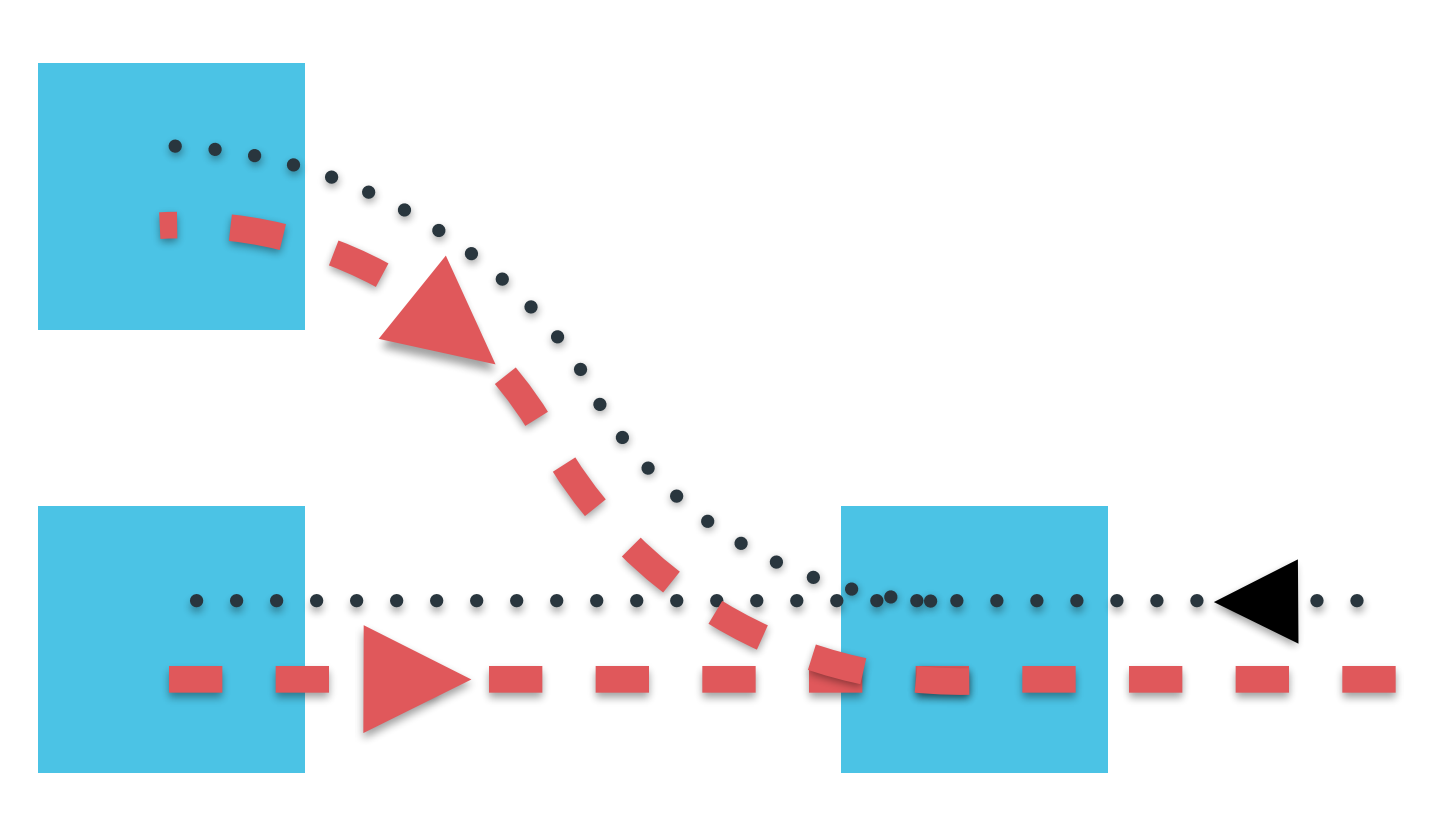
\includegraphics[scale=0.25]{imgs/merge.png} 
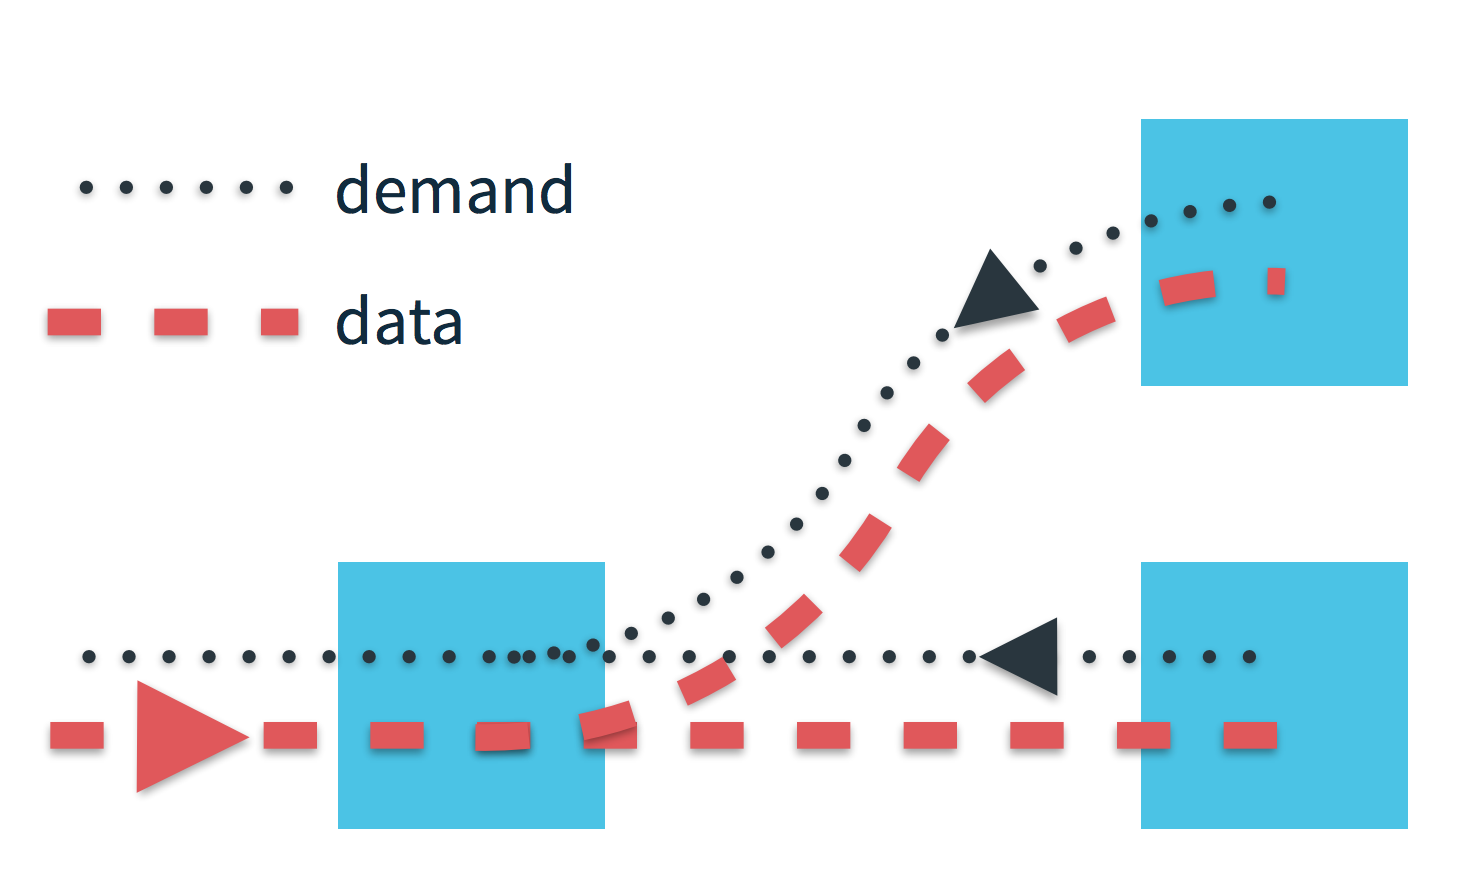
\includegraphics[scale=0.25]{imgs/split.png}

As the main document says, the scope of Reactive Streams is to find a
minimal set of interfaces, methods and protocols that will describe the
necessary operations and entities to achieve the goal---asynchronous
streams of data with non-blocking back pressure. This set of interfaces
are a low level specification to which each library should be conform
to.

The API offers the following interfaces that are required to be
implemented by each implementations:

\begin{itemize}
\itemsep1pt\parskip0pt\parsep0pt
\item
  Subscriber
\item
  Subscription
\item
  Publisher
\item
  Processor
\end{itemize}


\section{Subscriber}\label{subscriber}

The \textbf{Subscriber} interface abstracts the notion of an entity that
consumes items. Its definition is as follows.

\begin{verbatim}
public interface Subscriber<T> {
    public void onSubscribe(Subscription s);
    public void onNext(T t);
    public void onError(Throwable t);
    public void onComplete();
}
\end{verbatim}

A \texttt{Subscriber} has the canonical \texttt{onNext(\ )},
\texttt{onError(\ )}, and \texttt{onComplete()} methods. When new items
are produced by the publisher, a the onNext method is invoked with the
new element. If an error was raised while producing values, the
publisher would then invoke the onError method with the exception.
Finally, when the publisher completes its job, the onComplete method is
then invoked.

The \texttt{onSubscribe(\ )} method is invoked when a subscriber is
subscribed to a publisher. This method is really important for the
framework, since it links the relation between a subscriber and a
publisher, via a \texttt{Subscription}.

\section{Subscription}\label{subscription}

A \textbf{Subscription} abstracts the notion of a subscriber's
communication channel back to the publisher. This channel is what
enables the subscriber to either cancel the subscription or signal
demand. Its definition is as follows.

\begin{verbatim}
public interface Subscription {
    public void request(long n);
    public void cancel();
}
\end{verbatim}

The \texttt{request(\ )} method signals to the publisher that the
subscriber can receive more items, also specifying the quantity.

The \texttt{cancel(\ )} method notifies the publisher that the
subscriber is no longer interested in receiving items.

This channel between a publisher and a subscriber is what enables to
achieve non blocking back-pressure in a Reactive Streams.

\section{Publisher}\label{publisher}

The \textbf{Publisher} interface has only one method to implement, and
is as follows.

\begin{verbatim}
public interface Publisher<T> {
    public void subscribe(Subscriber<? super T> s);
}
\end{verbatim}

A subscriber is subscribed to a publisher via the \texttt{subscribe(\ )}
method. This method doesn't return a \texttt{Subscription} as one would
expect, but \texttt{Unit}. This is a precise design choice, since every
method of the interfaces returns \texttt{Unit}.

The publisher, after notifying the subscriber that it has been
subscribed via its \texttt{onSubscribed(\ )} method, must provide items
to the subscriber, that will receive items in its \texttt{onNext(\ )}
method. The items received must not exceed the total number of items
that the subscriber has signalled demand for.

When the subscriber \texttt{cancel(\ )} the subscription, the publisher
must start sending items.

Finally, a publisher must notify to the subscriber through
\texttt{onError(\ )} and \texttt{onComplete(\ )} methods if an error is
encountered or the stream is successfully completed respectively.

\section{Processor}\label{processor}

A \textbf{Processor} represents a processing stage, which is both a
Subscriber and a Publisher and obeys the contracts of both. The
interface is defined as follows.

\begin{verbatim}
public interface Processor<T, R>
    extends Subscriber<T>, Publisher<R> { }
\end{verbatim}

A processor is an intermediate abstraction that enables to build
\textbf{chain of processing stage}, in which each intermediate unit is a
processor that can consume, transform and publish items. The importance
of this abstraction is in the fact that, obeying to both Subscriber and
Publisher interface, it has to \textbf{retain back-pressure
propagation} with the original stream source.





%\chapter*{Ringraziamenti}


%%%%%%%%%%%%%%%%%%%%%%%%%
% inizio parte finale del documento
%
% eventuali appendici, bibliografia obbligatoria,
% eventuale lista delle tabelle e delle figure (nel caso decommentare la riga con i comandi \listoffigures e \listoftables)
%%%%%%%%%%%%%%%%%%%%%%%%%
\backmatter


%\input{./Appendice/appendice.tex}
% \input{./Bibliografia/bibliografia.tex}

\bibliography{biblio}
\bibliographystyle{abbrv}

%\listoffigures
%\listoftables

% chiusura del documento
\end{document}
